\chapter{\ifproject%
\ifcpe โครงสร้างและขั้นตอนการทำงาน\else Project Structure and Methodology\fi
\else%
\ifcpe โครงสร้างของโครงงาน\else Project Structure\fi
\fi
}



\section{โครงสร้างของระบบ}



\subsection{Database Design}

ประเภทของฐานข้อมูลที่ใช้เป็นแบบ NoSQL
(รูปที่~\ref{fig:DatabaseDiagram}) แสดงองค์ประกอบต่างๆ ของฐานข้อมูล ซึ่งมีรายละเอียดดังต่อไปนี้
%
  \begin{itemize}
    \item childs เก็บข้อมูลที่เกี่ยวข้องกับเด็กทั้งหมด เช่น เก็บวันที่สมัคร วันที่เข้าเรียน ชื่อ ชื่อเล่น วันเดือนปีเกิด เป็นต้น  
    โดยที่ \_id จะมีการเชื่อมกับ payment, gadgets, healths, enrollment, address, guardians, customer, childStatic, childDynamic, medical, document, child\_info 
    ในส่วนของการเชื่อมความสัมพันธ์นี้ ทำเพื่อให้การเรียกใช้ข้อมูลของเด็กในส่วนของข้อมูลอื่น เช่น การเช็คชื่อ การชำระเงินค่าเรียน การเช็คของ เกิดขึ้นได้โดยสะดวกยิ่งขึ้น
    \item childStatic เก็บข้อมูลเด็กที่ไม่เปลี่ยนแปลง เช่น เชื้อชาติ ศาสนา วันที่สมัคร
    \item childDynamic เก็บข้อมูลเด็กที่มีการเปลี่ยนแปลง เช่น น้ำหนัก ส่วนสูง รูปถ่าย
    \item child\_info เก็บข้อมูลพฤติกรรมต่างๆ ของเด็ก
    \item info\_category เก็บข้อมูลชื่อประเภทหัวเรื่องต่างๆ
    \item info\_item เก็บข้อมูลหยิบย่อยต่างๆ
    \item info\_display\_order เก็บข้อมูลสำหรับทำหน้าแสดงผลแบบ dynamic
    \item customer เก็บข้อมูลลูกค้าสำหรับใช้ซื้อของจากทางเนอสเซอรี่
    \item medical เก็บข้อมูลทางการแพทย์ของเด็ก
    \item document เก็บข้อมูลเอกสารในการสมัครของเด็ก
    \item guardians เก็บข้อมูลส่วนตัวของผู้ปกครองเด็ก เช่น ชื่อ ทำอาชีพอะไร อีเมล เบอร์โทร มีความสัมพันธ์อะไรกับเด็ก เป็นต้น
    \item address เก็บข้อมูลที่อยู่ของเด็ก เช่น บ้านเลขที่ ถนน ตำบล อำเภอ จังหวัด รหัสไปรษณีย์ 
    \item users เก็บ email password สำหรับเข้าสู่ ระบบจัดการ nursery 
    \item rooms เก็บข้อมูลห้องเรียนว่าห้องนี้ชื่อห้องว่าอะไร ไว้ให้ enrollment เรียกใช้ผ่าน ObjectId
    \item enrollment เก็บข้อมูลว่าเด็กเริ่มเรียนห้องนี้วันไหน มีการย้ายออกจากห้องนี้วันไหน
    \item attendances เก็บข้อมูลการเช็คชื่อทั้งหมด วันที่เช็ค สถานะว่ามาหรือไม่มา
    \item gadgets เก็บข้อมูลการเช็คอุปกรณ์ของเด็กทั้งหมด มีการเก็บ ข้อมูลเด็ก วัน ลิสต์ของที่ต้องเช็ค ก็จะมีสถานะว่าเอามาหรือไม่เอามา
    \item healths เก็บข้อมูลการเช็คสุขภาพของเด็กทั้งหมด มีการเก็บ ข้อมูลเด็ก วัน ลิสต์สุขภาพที่ต้องเช็ค ก็จะมีสถานะว่าใช่หรือไม่ใช่
    \item stock เก็บข้อมูลของใช้ทั้งหมดของเด็กใน nursery ว่าของชิ้นนี้ชื่ออะไร ขนาดเท่าไหร่ รหัสสินค้าคืออะไร
    \item show\_stock เก็บข้อมูลว่าของต่างละอย่างในคลังสินค้า มีจำนวนกี่ชิ้น ราคาเท่าไหร่
    \item history\_stock เก็บข้อมูลการเพิ่มลดของต่างๆจำนวนของในคลังสินค้า แก้ไขวันไหน โดยใคร
    \item payment เก็บข้อมูลประวัติการโอนเงินค่าเล่าเรียนของผู้ปกครองเด็ก มีการเก็บ ข้อมูลเด็ก วันที่ส่งสลิปโอนเงิน ค่าเล่าเรียนหรือจำนวนเงินที่ชำระ รูปสลิปใบเสร็จ 
  \end{itemize}
\CIreply{ฝากมึงจัดรูปให้เข้าที่เข้าทางด้วยนะ}
\subsection{XD Design}

\begin{itemize}
  \item RegisterPage คือ หน้าแบบฟอร์มในการลงทะเบียนเด็กในการเข้าเรียน nursery 
  
  ซึ่งระบบนี้เป็นแบบ StepForm คือกรอกแล้วสามารถกลับมาแก้ไขข้อมูลเดิมได้ หากผู้ใช้ยังไม่กดยืนยันข้อมูลใน stepสุดท้าย
  เริ่มแรกผู้ใช้จะต้องกรอกข้อมูลส่วนตัวของเด็ก(รูปที่~\ref{fig:register}) 
  
  จากนั้นก็กรอกประวัติผู้ปกครอง (รูปที่~\ref{fig:fatherForm}, \ref{fig:motherForm}, \ref{fig:guardiansForm})
  
  สุดท้ายผู้ใช้จะต้องกรอกข้อมูลที่อยู่ของเด็ก(รูปที่~\ref{fig:addressForm}) เมื่อกรอกข้อมูลทั้งหมดเสร็จสิ้นให้กดปุ่มยืนยันเพื่อบันทึกผล
  
    \begin{figure}
      \begin{center}
      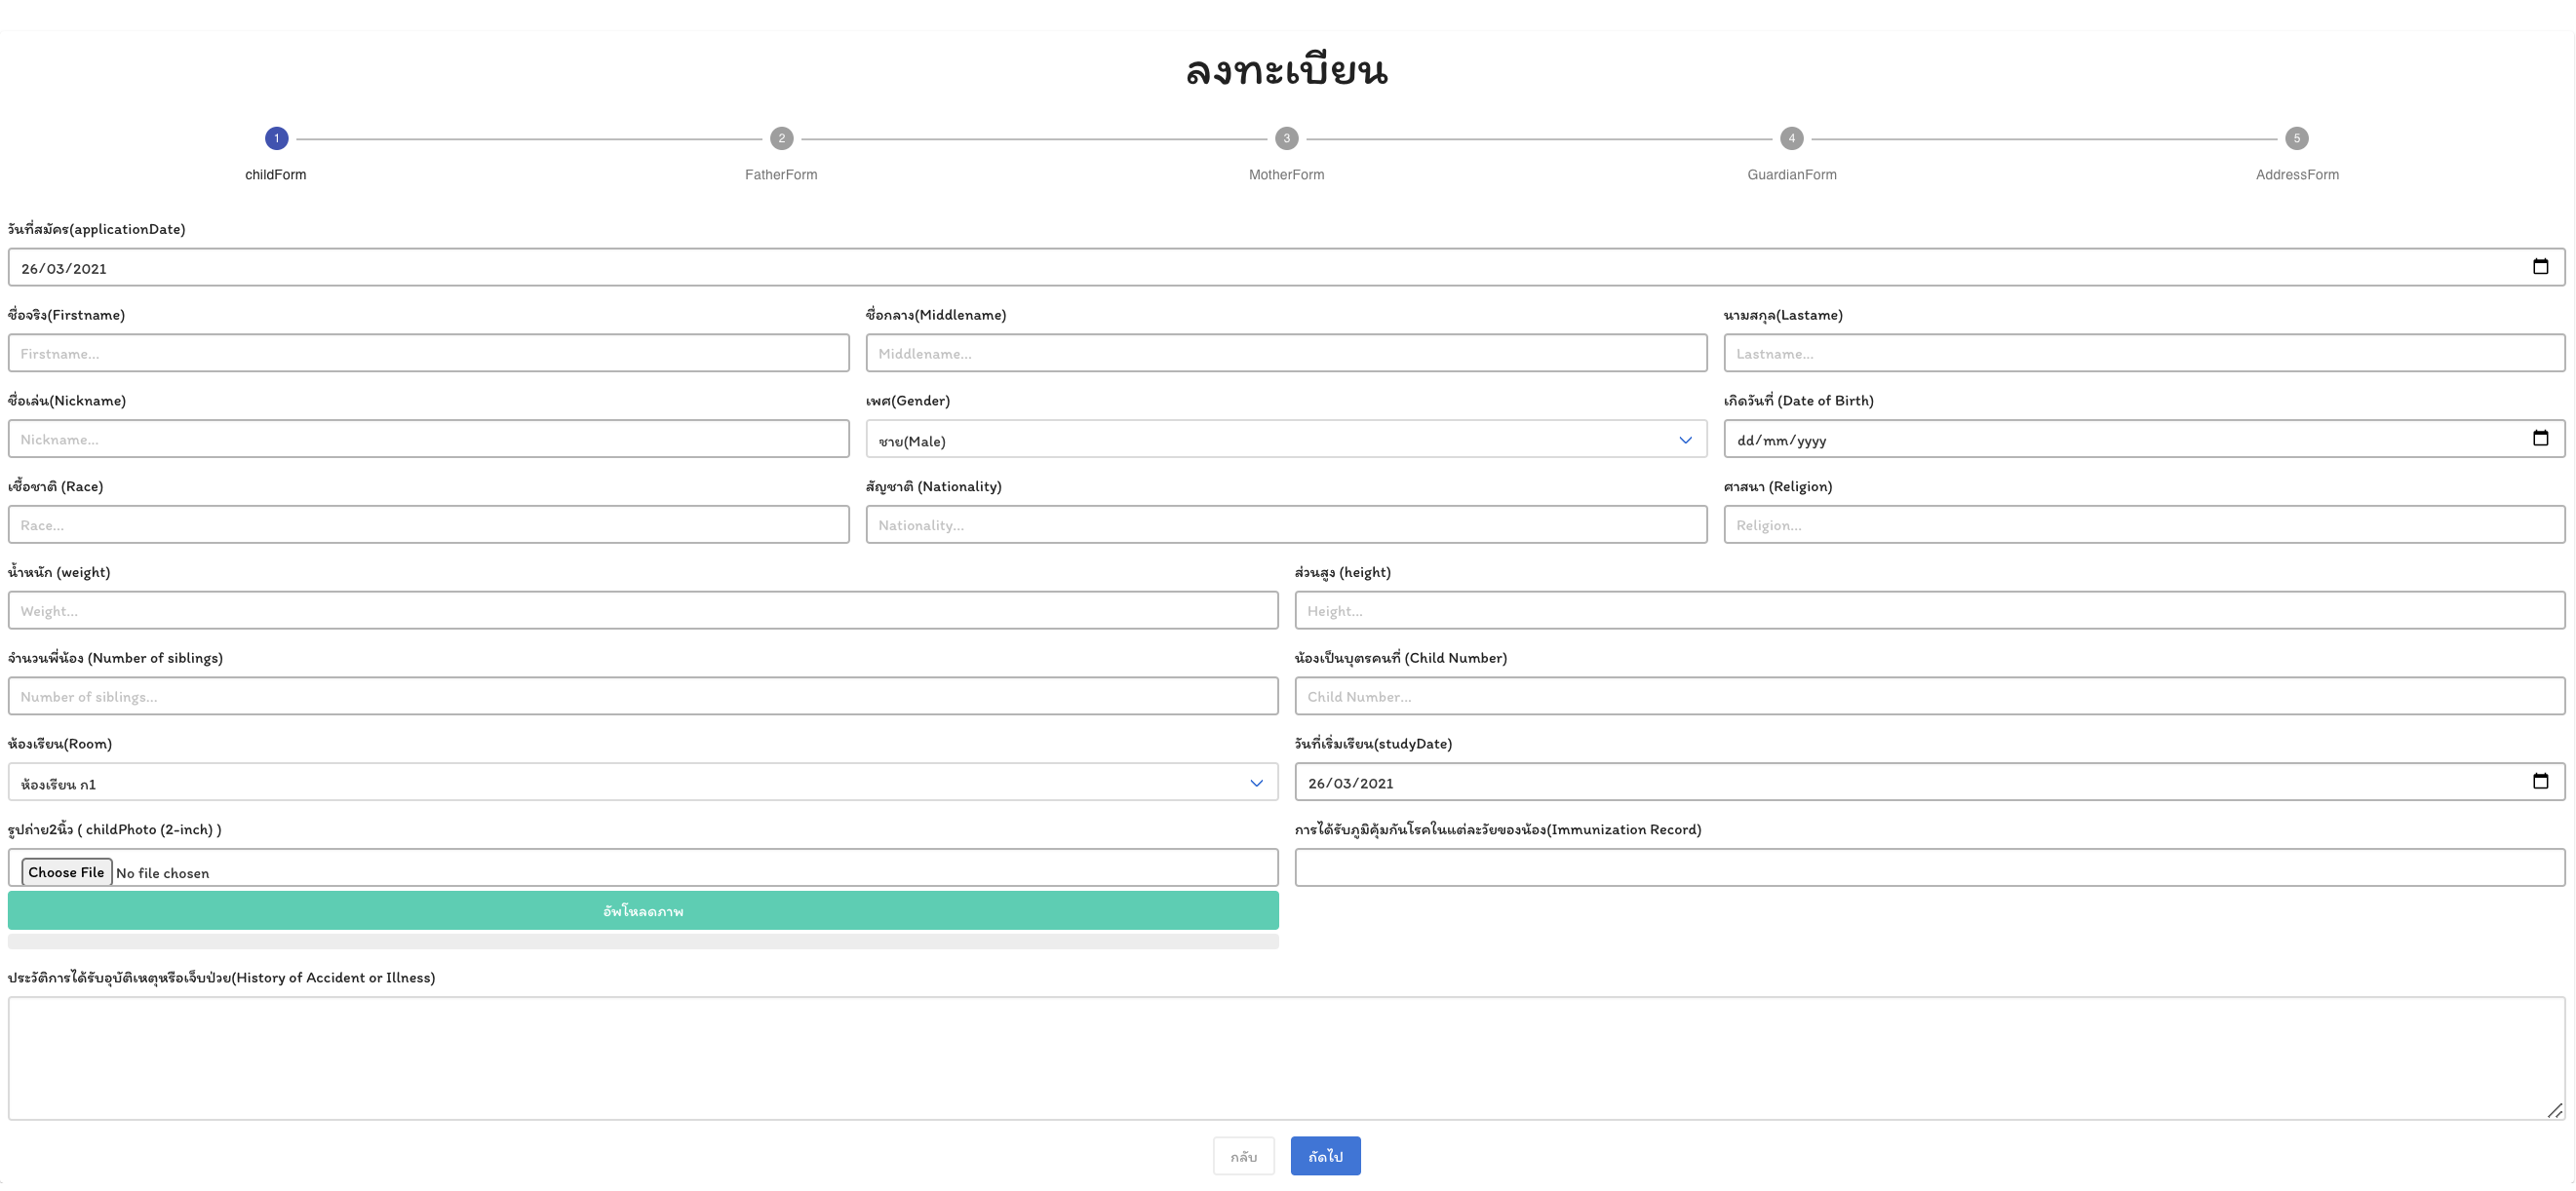
\includegraphics[width=\linewidth]{images/RegisterForm.png}
      \end{center}
      \caption[หน้ากรอกข้อมูลเด็ก]{หน้ากรอกข้อมูลเด็ก}
      \label{fig:register}
    \end{figure}
  
  
    \begin{figure}
      \begin{center}
      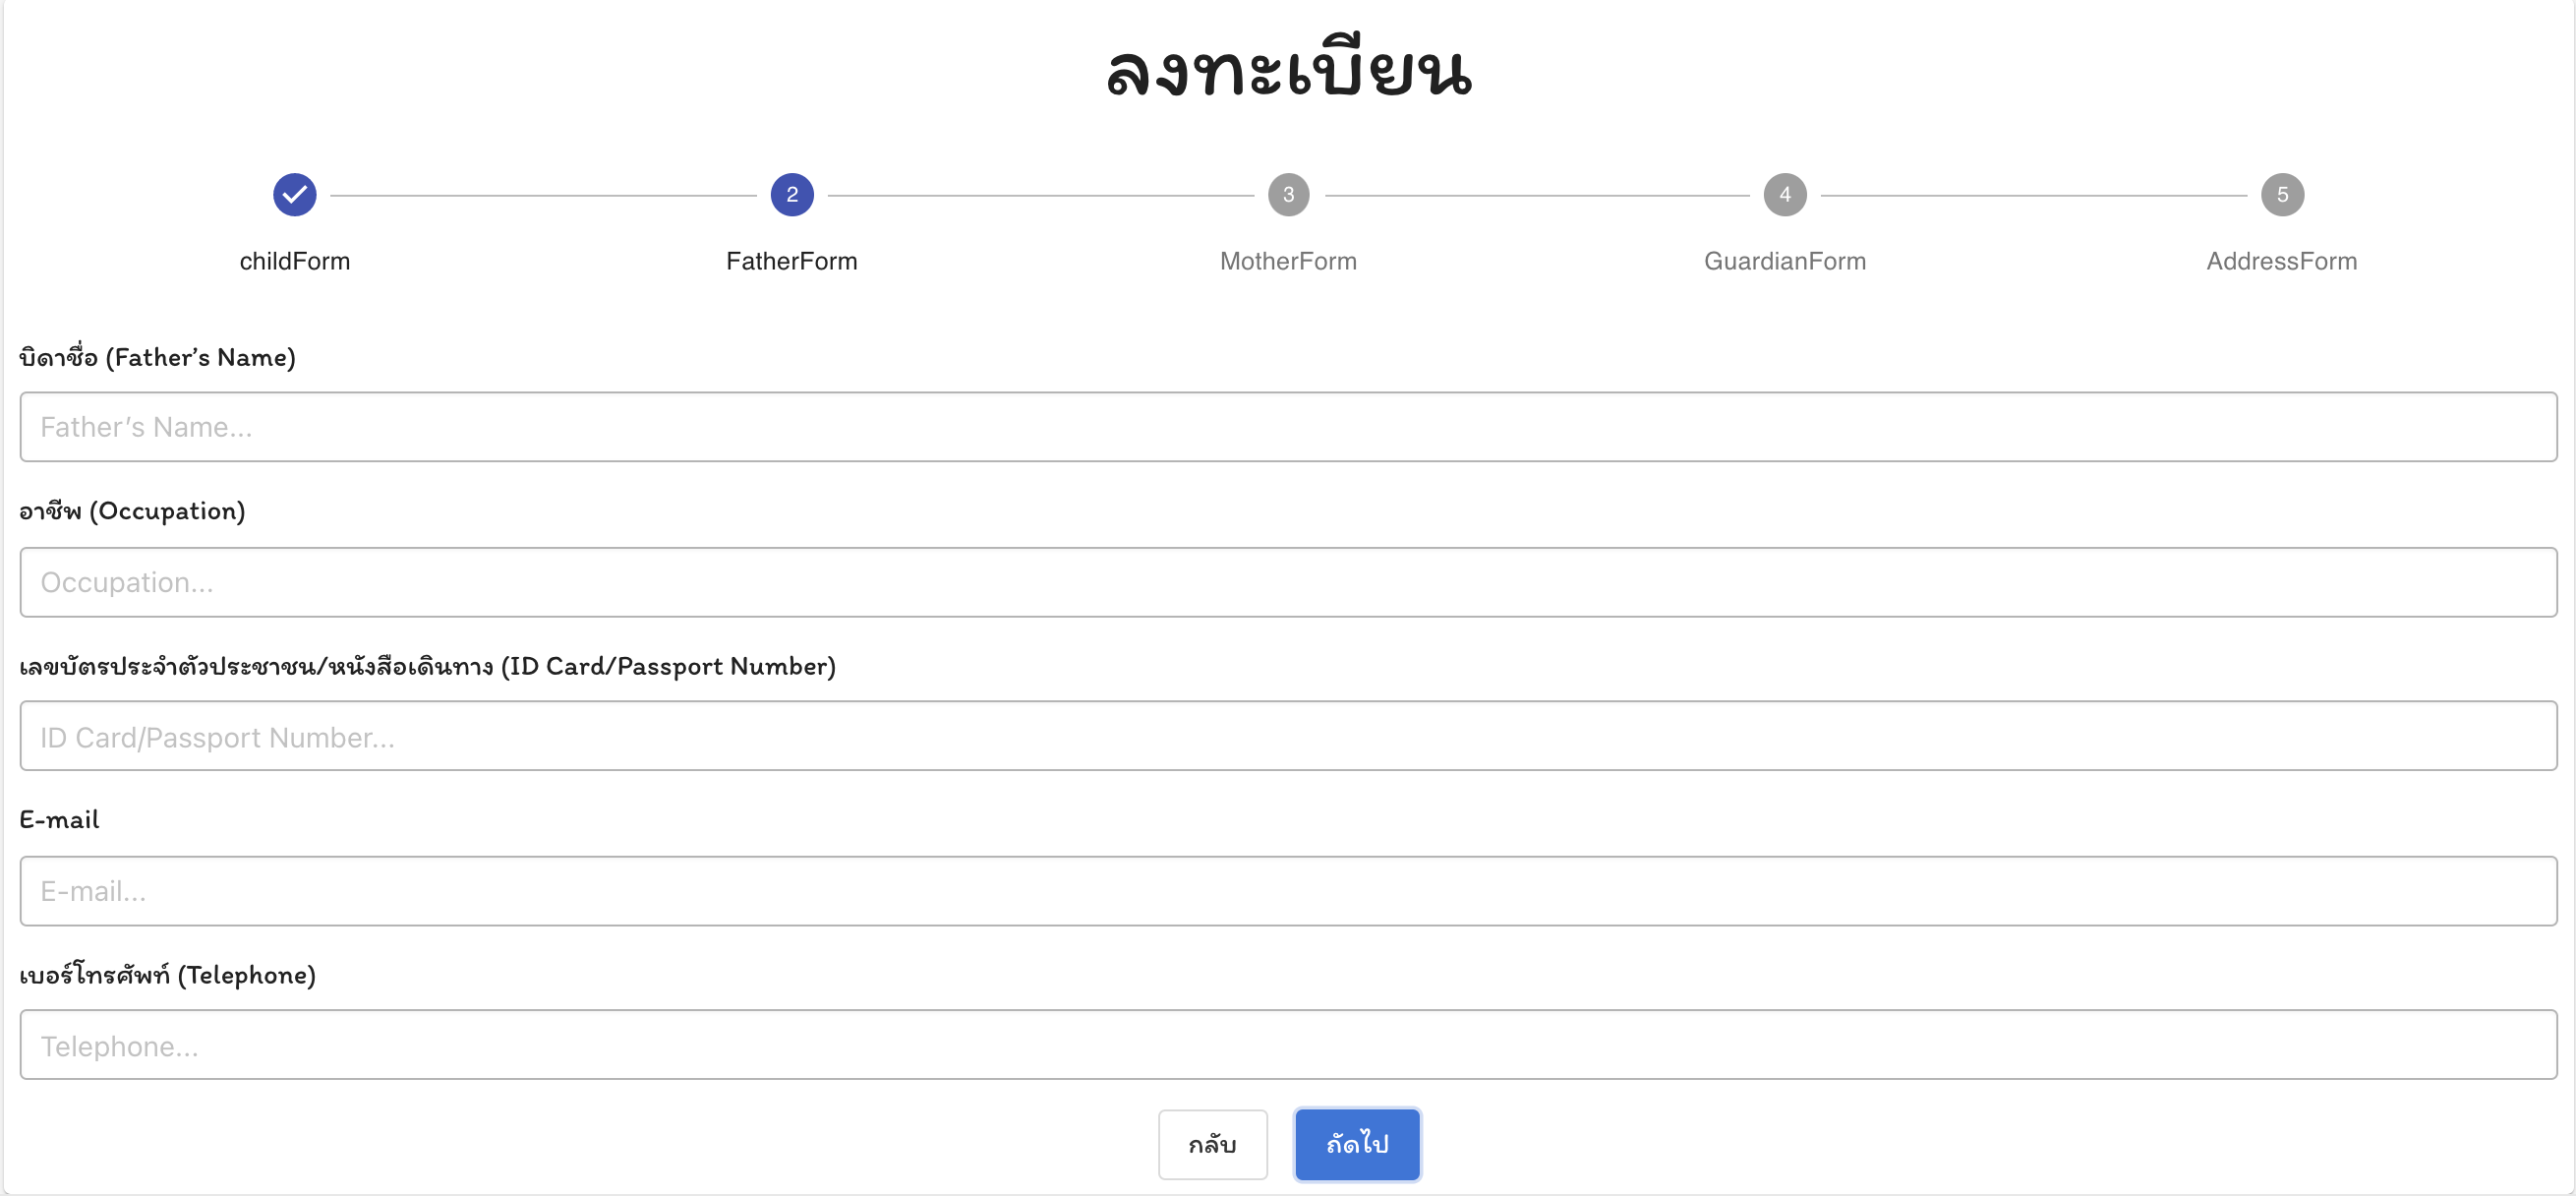
\includegraphics[width=\linewidth]{images/fatherForm.png}
      \end{center}
      \caption[หน้ากรอกข้อมูลบิดา]{หน้ากรอกข้อมูลบิดา}
      \label{fig:fatherForm}
    \end{figure}
  
  
    \begin{figure}
      \begin{center}
      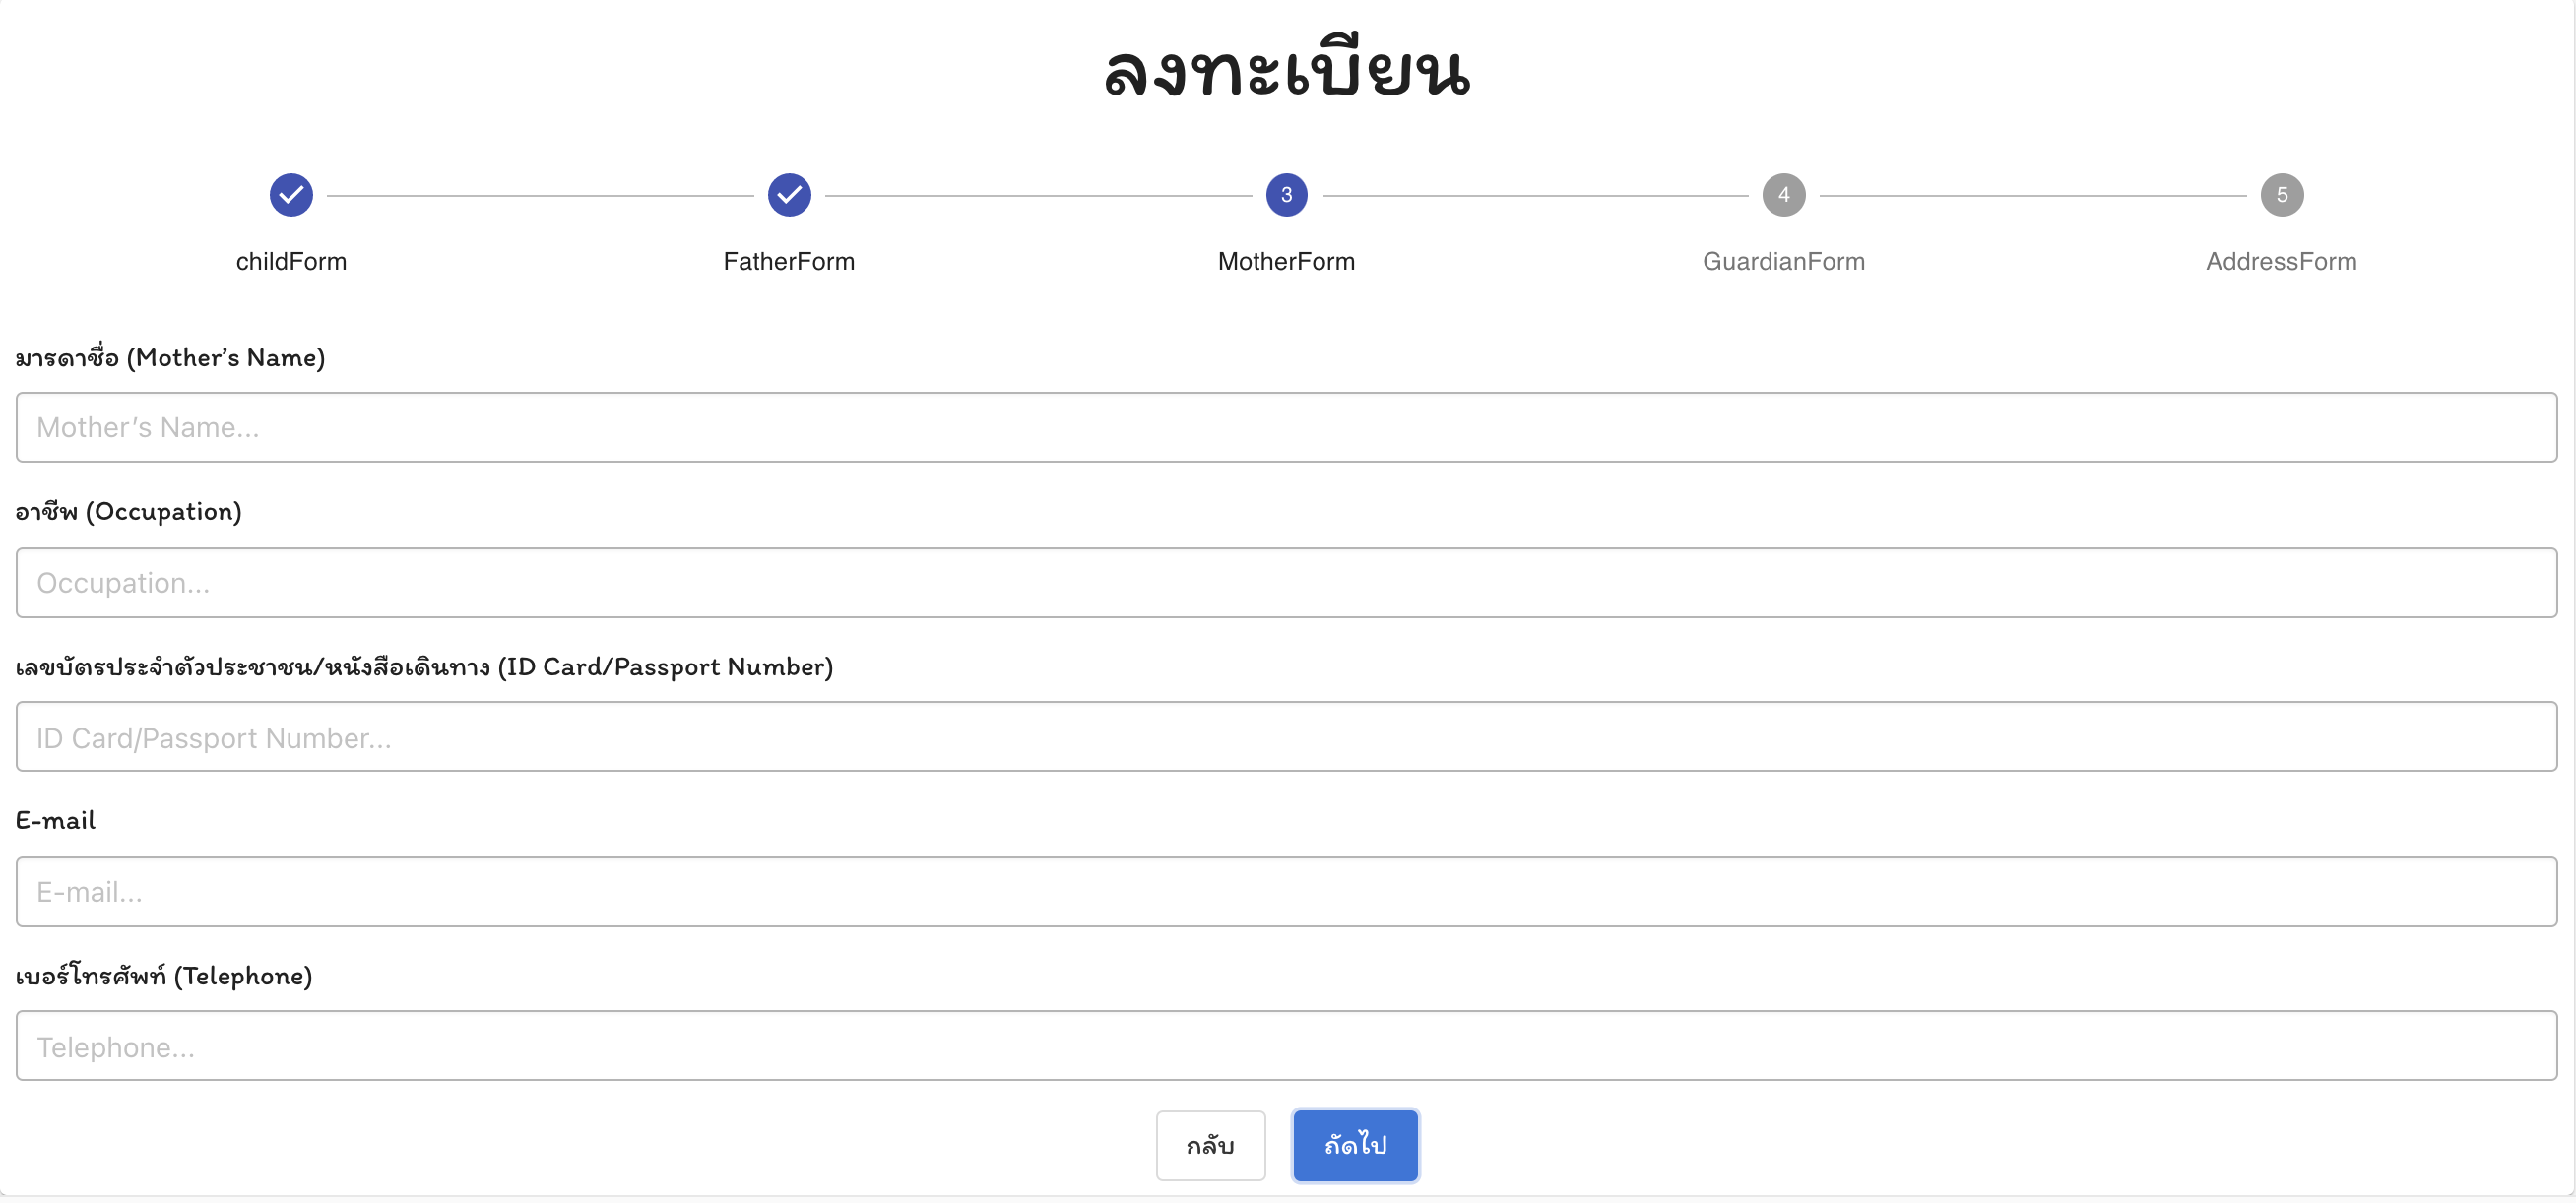
\includegraphics[width=\linewidth]{images/motherForm.png}
      \end{center}
      \caption[หน้ากรอกข้อมูลมารดา]{หน้ากรอกข้อมูลมารดา}
      \label{fig:motherForm}
    \end{figure}
  
  
    \begin{figure}
      \begin{center}
      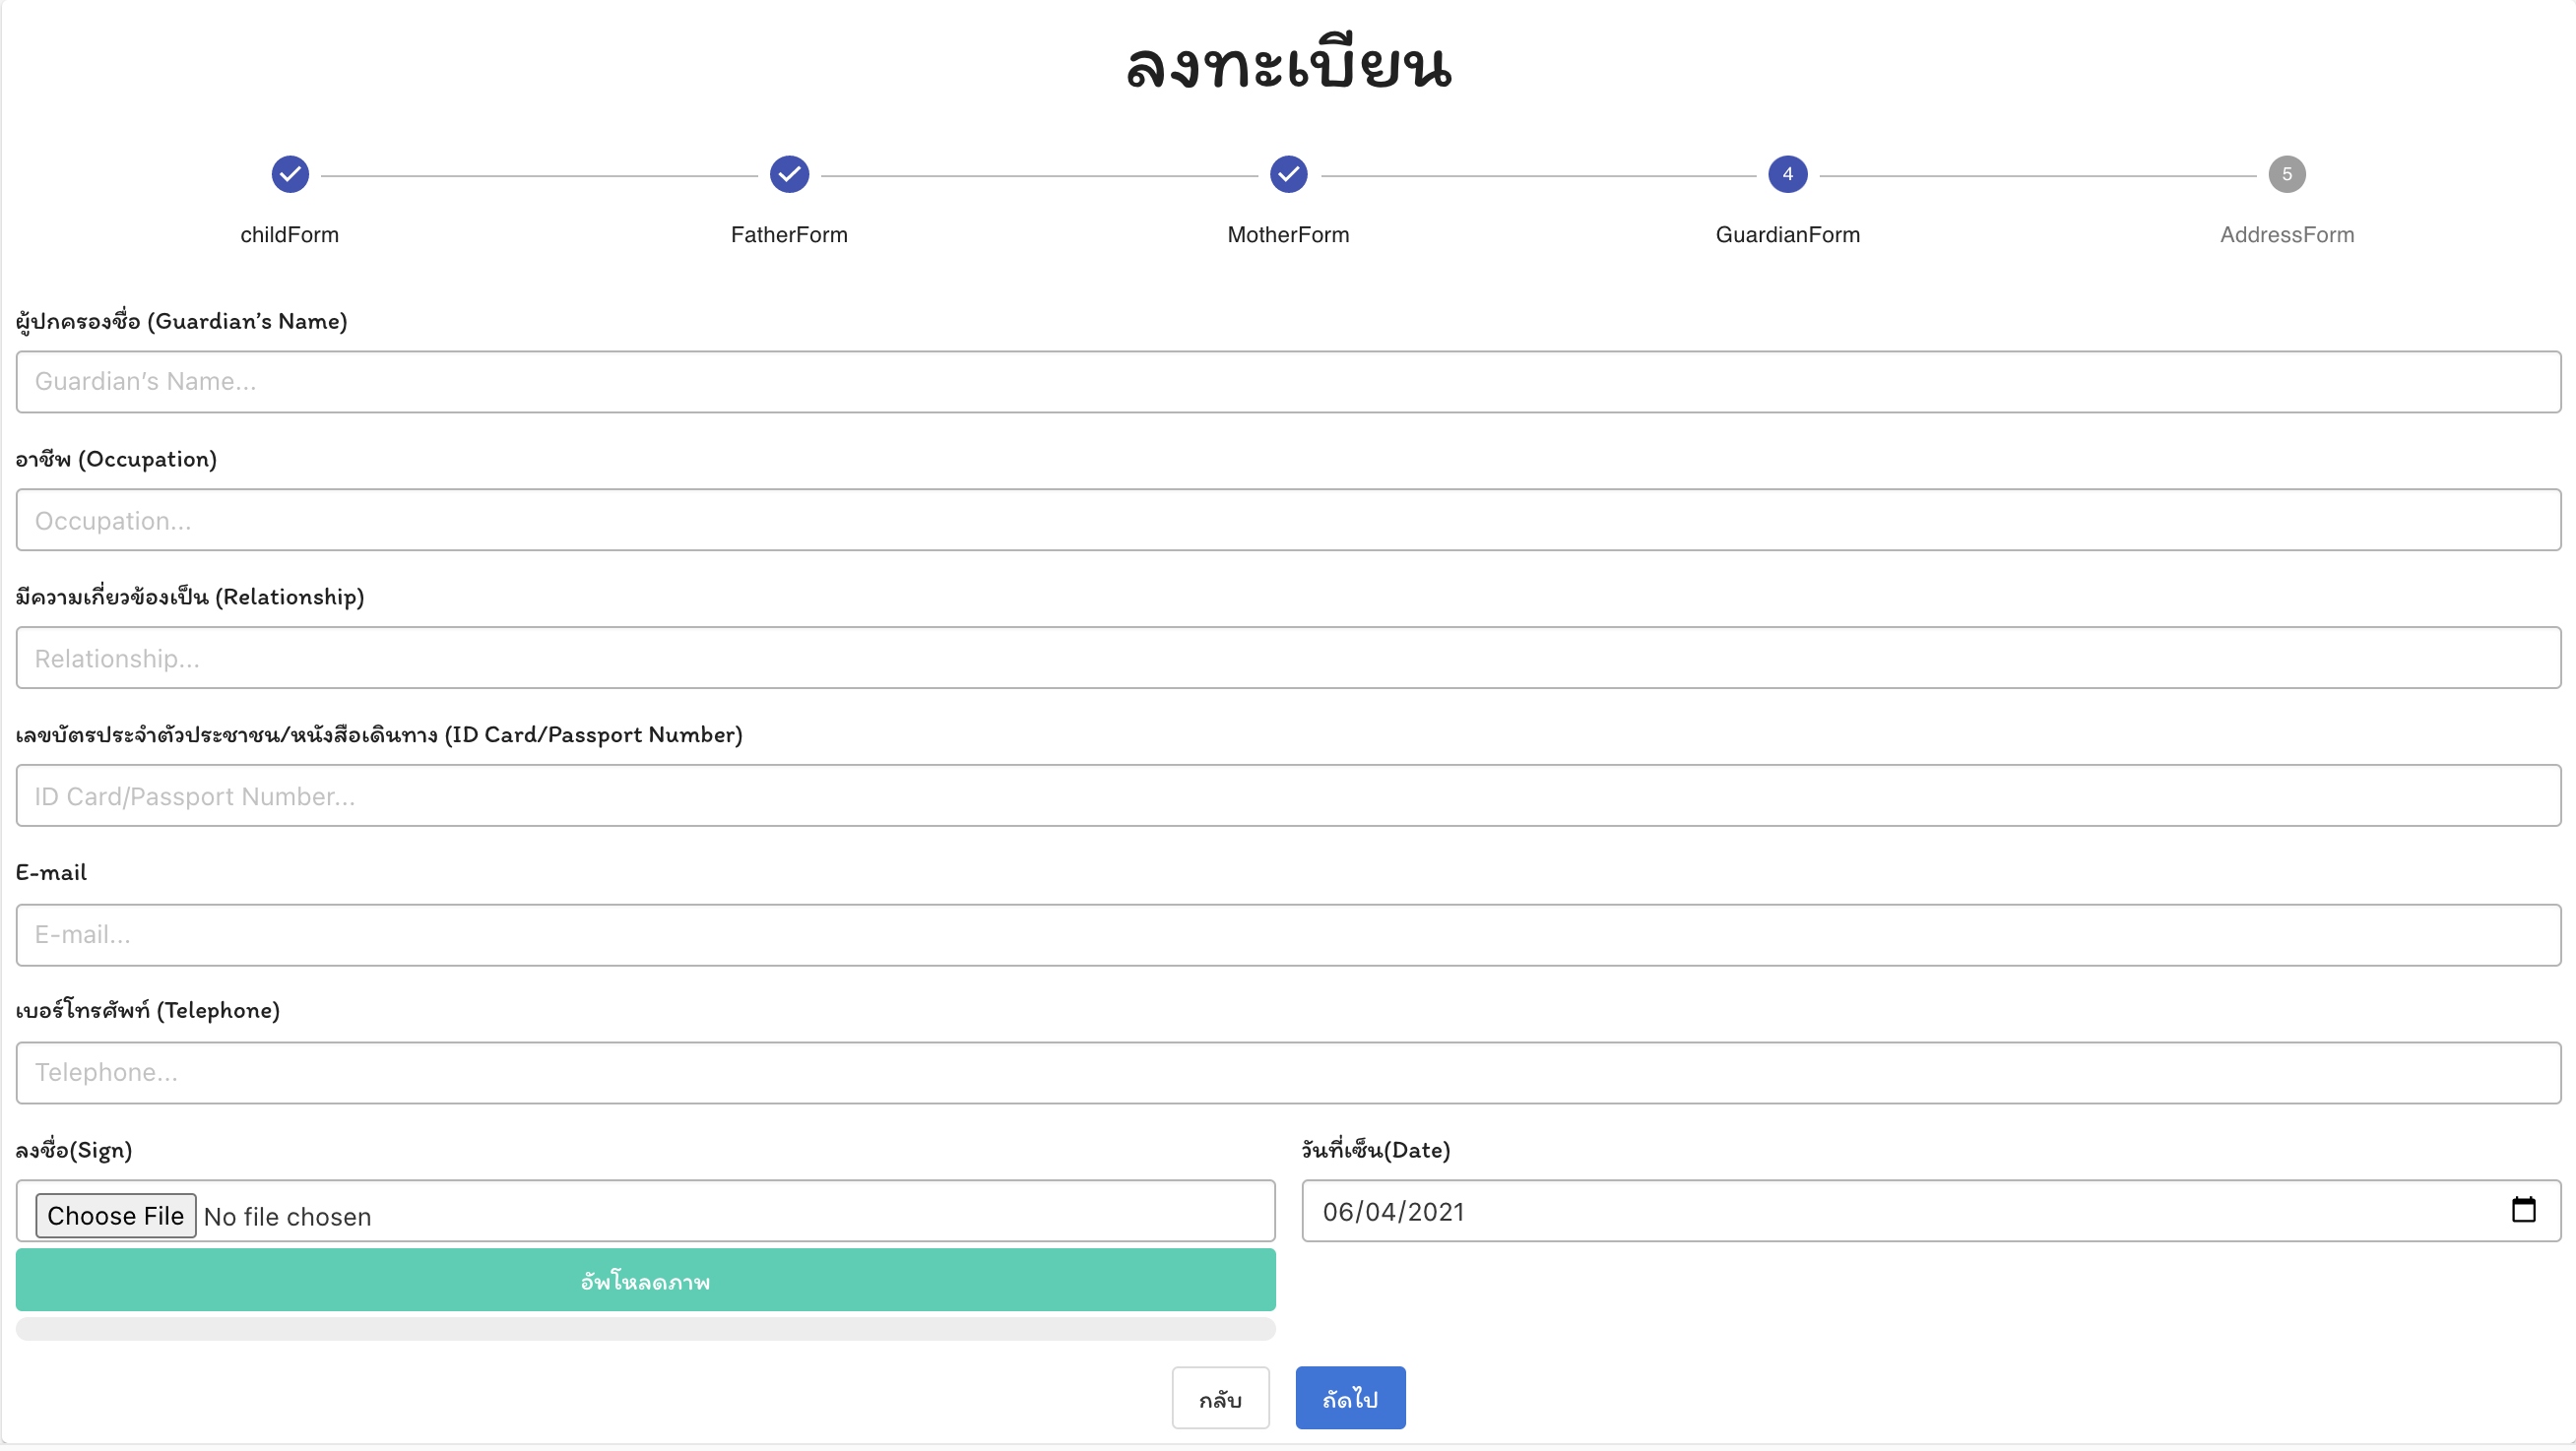
\includegraphics[width=\linewidth]{images/guardiansForm.png}
      \end{center}
      \caption[หน้ากรอกข้อมูลผู้ปกครอง]{หน้ากรอกข้อมูลผู้ปกครอง}
      \label{fig:guardiansForm}
    \end{figure}
  
  
    \begin{figure}
      \begin{center}
      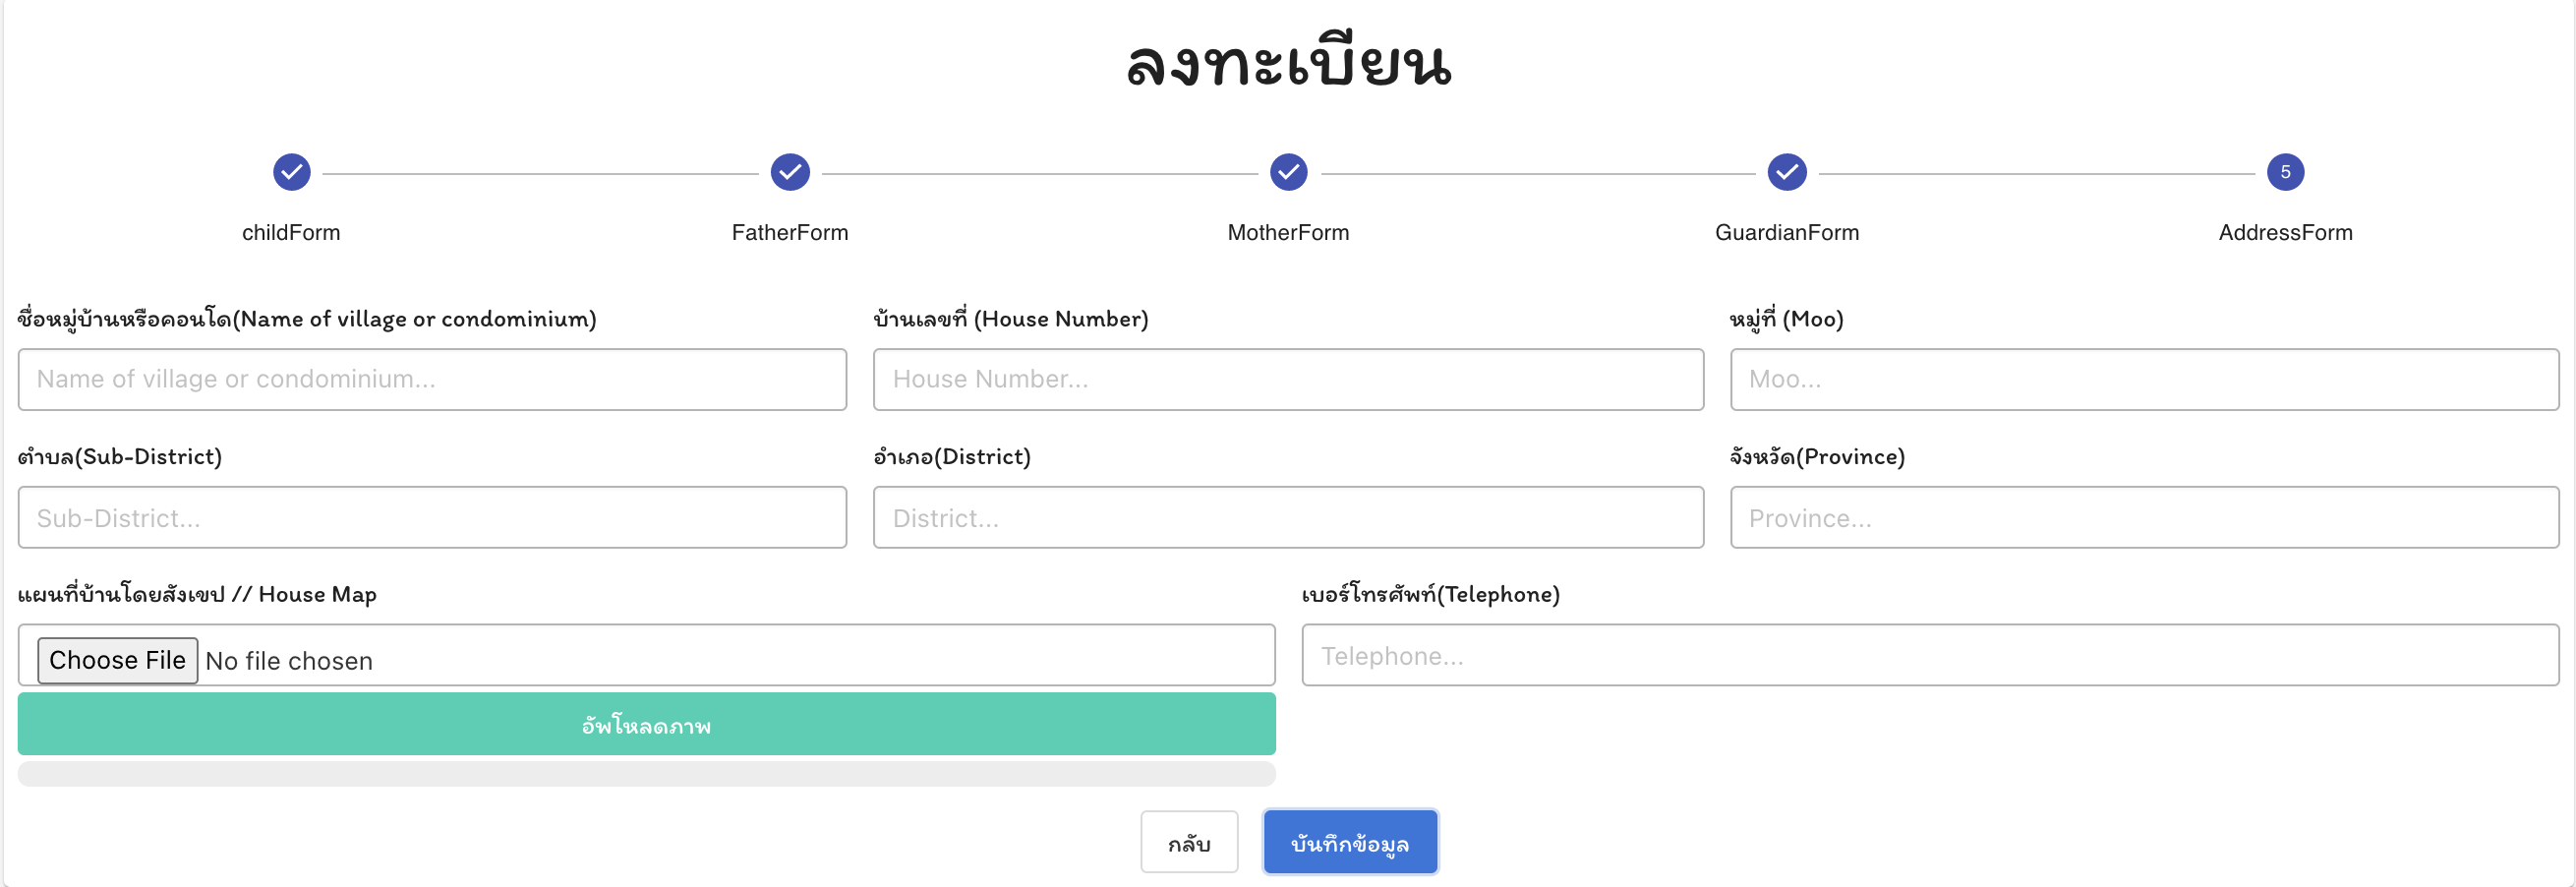
\includegraphics[width=\linewidth]{images/addressForm.png}
      \end{center}
      \caption[หน้ากรอกข้อมูลที่อยู่]{หน้ากรอกข้อมูลที่อยู่}
      \label{fig:addressForm}
    \end{figure}
  
  
  \item  ProfilePage คือ หน้าที่ใช้ในการจัดการกับประวัติส่วนตัวของเด็ก(รูป~\ref{fig:Profile}) ซึ่งจะมีฟังก์ชั่นการทำงานเสริมที่ใช้ดูประวัติส่วนตัวกับข้อมูลรายเดือนของเด็ก
  โดยกดปุ่มสีฟ้าใต้ชื่อเพื่อดูข้อมูลส่วนตัว(รูป~\ref{fig:ProfileTwo}) ซึ่งหน้านี้จะแสดงข้อมูลส่วนตัวและสามารถแก้ไขข้อมูลของเด็กแต่ละคนได้โดยกดปุ่มแก้ข้อมูล เมื่อกดแล้วระบบจะนำผู้ใช้ไปยังหน้า (รูป~\ref{fig:UpdateProfile}) 
  ในส่วนของหน้านี้จะสามารถแก้ไขน้ำหนัก ส่วนสูง ชื่อเล่น ห้องเรียน ชื่อและเบอร์โทรผู้ปกครอง(พ่อ,แม่,ญาติ) โรงพยาบาลที่จะให้พาน้องไปยามฉุกเฉิน รูปภาพน้อง 
  โดยที่สามารถแก้ไขบางส่วนได้ ไม่จำเป็นต้องแก้ไขข้อมูลทั้งหมดทุกครั้ง 
  ส่วนการใช้งานฟังก์ชั่นการแสดงข้อมูลรายเดือนของเด็กให้กลับมาที่หน้าประวัติ จากนั้นกดปุ่มสีชมพูล่างชื่อเด็ก
  จากนั้นระบบจะนำผู้ใช้มายังหน้าแสดงข้อมูลรายเดือน(รูป~\ref{fig:ChartPage})ของเด็กคนที่กดเลือก โดยที่การใช้งานหน้านี้จะมีให้เลือกเดือนที่จะดูข้อมูล เพียงเท่านี้

  
    \begin{figure}
      \begin{center}
      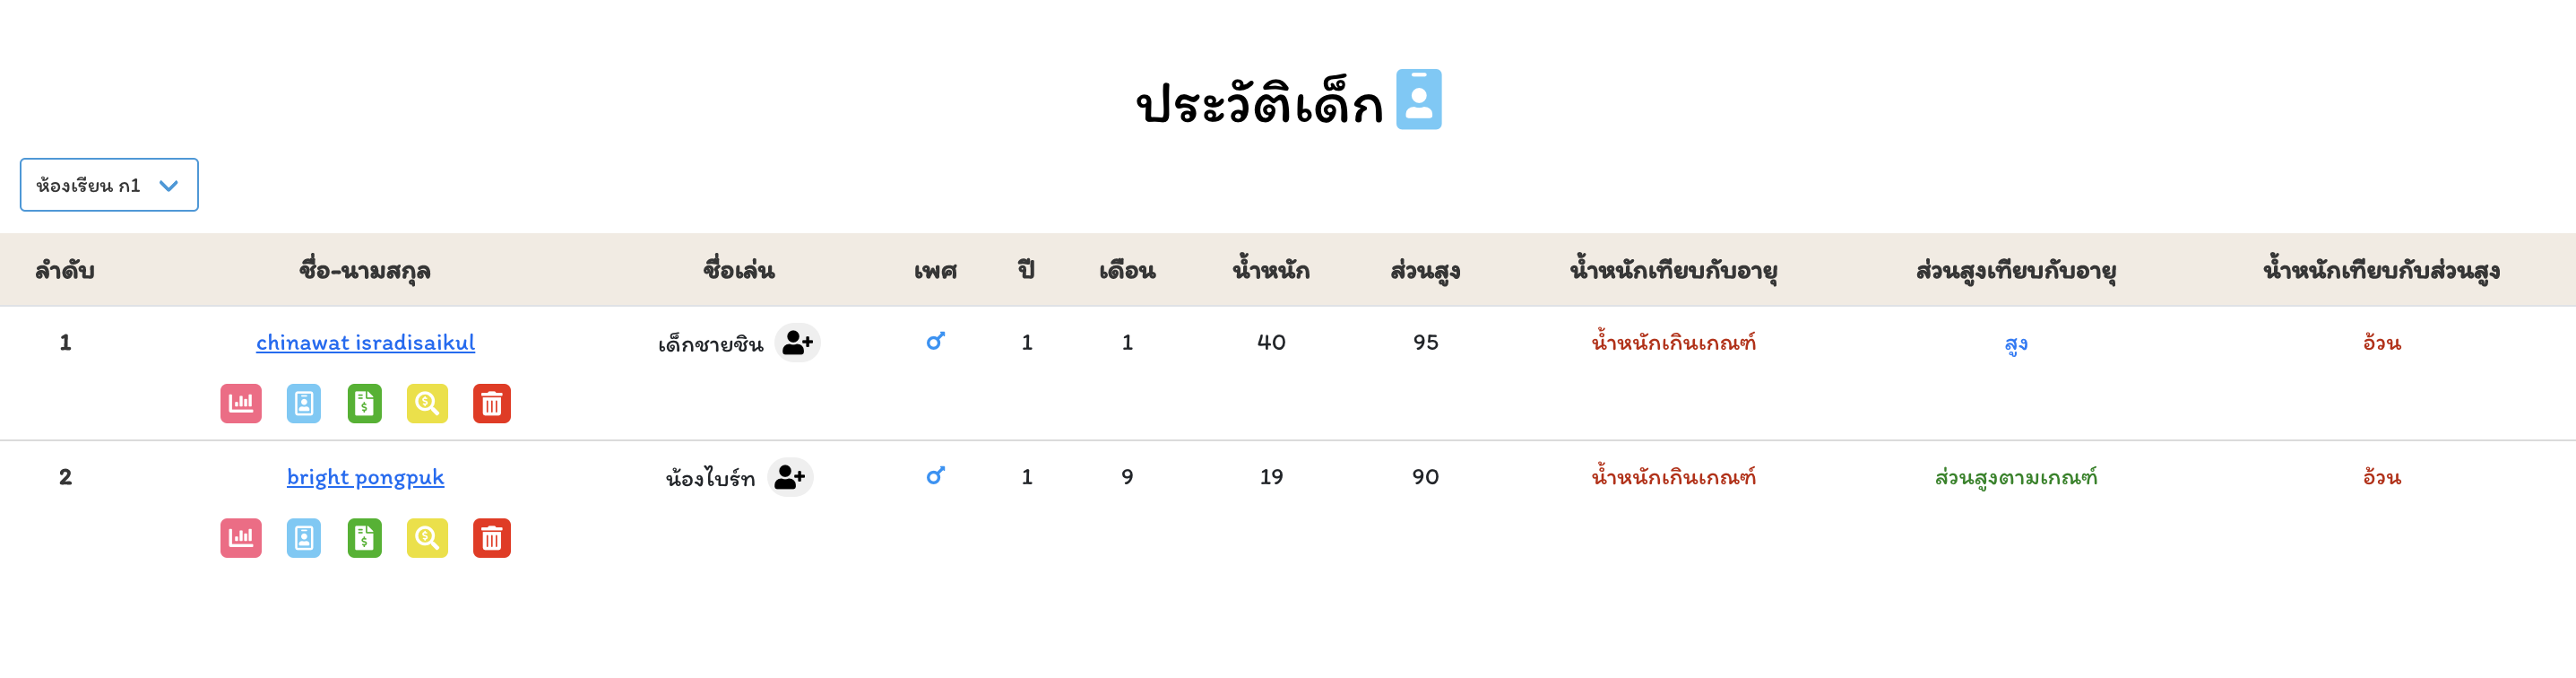
\includegraphics[width=\linewidth]{images/Profile.png}
      \end{center}
      \caption[หน้าประวัติเด็ก]{หน้าประวัติเด็ก}
      \label{fig:Profile}
    \end{figure}
  
  
  
    \begin{figure}
      \begin{center}
      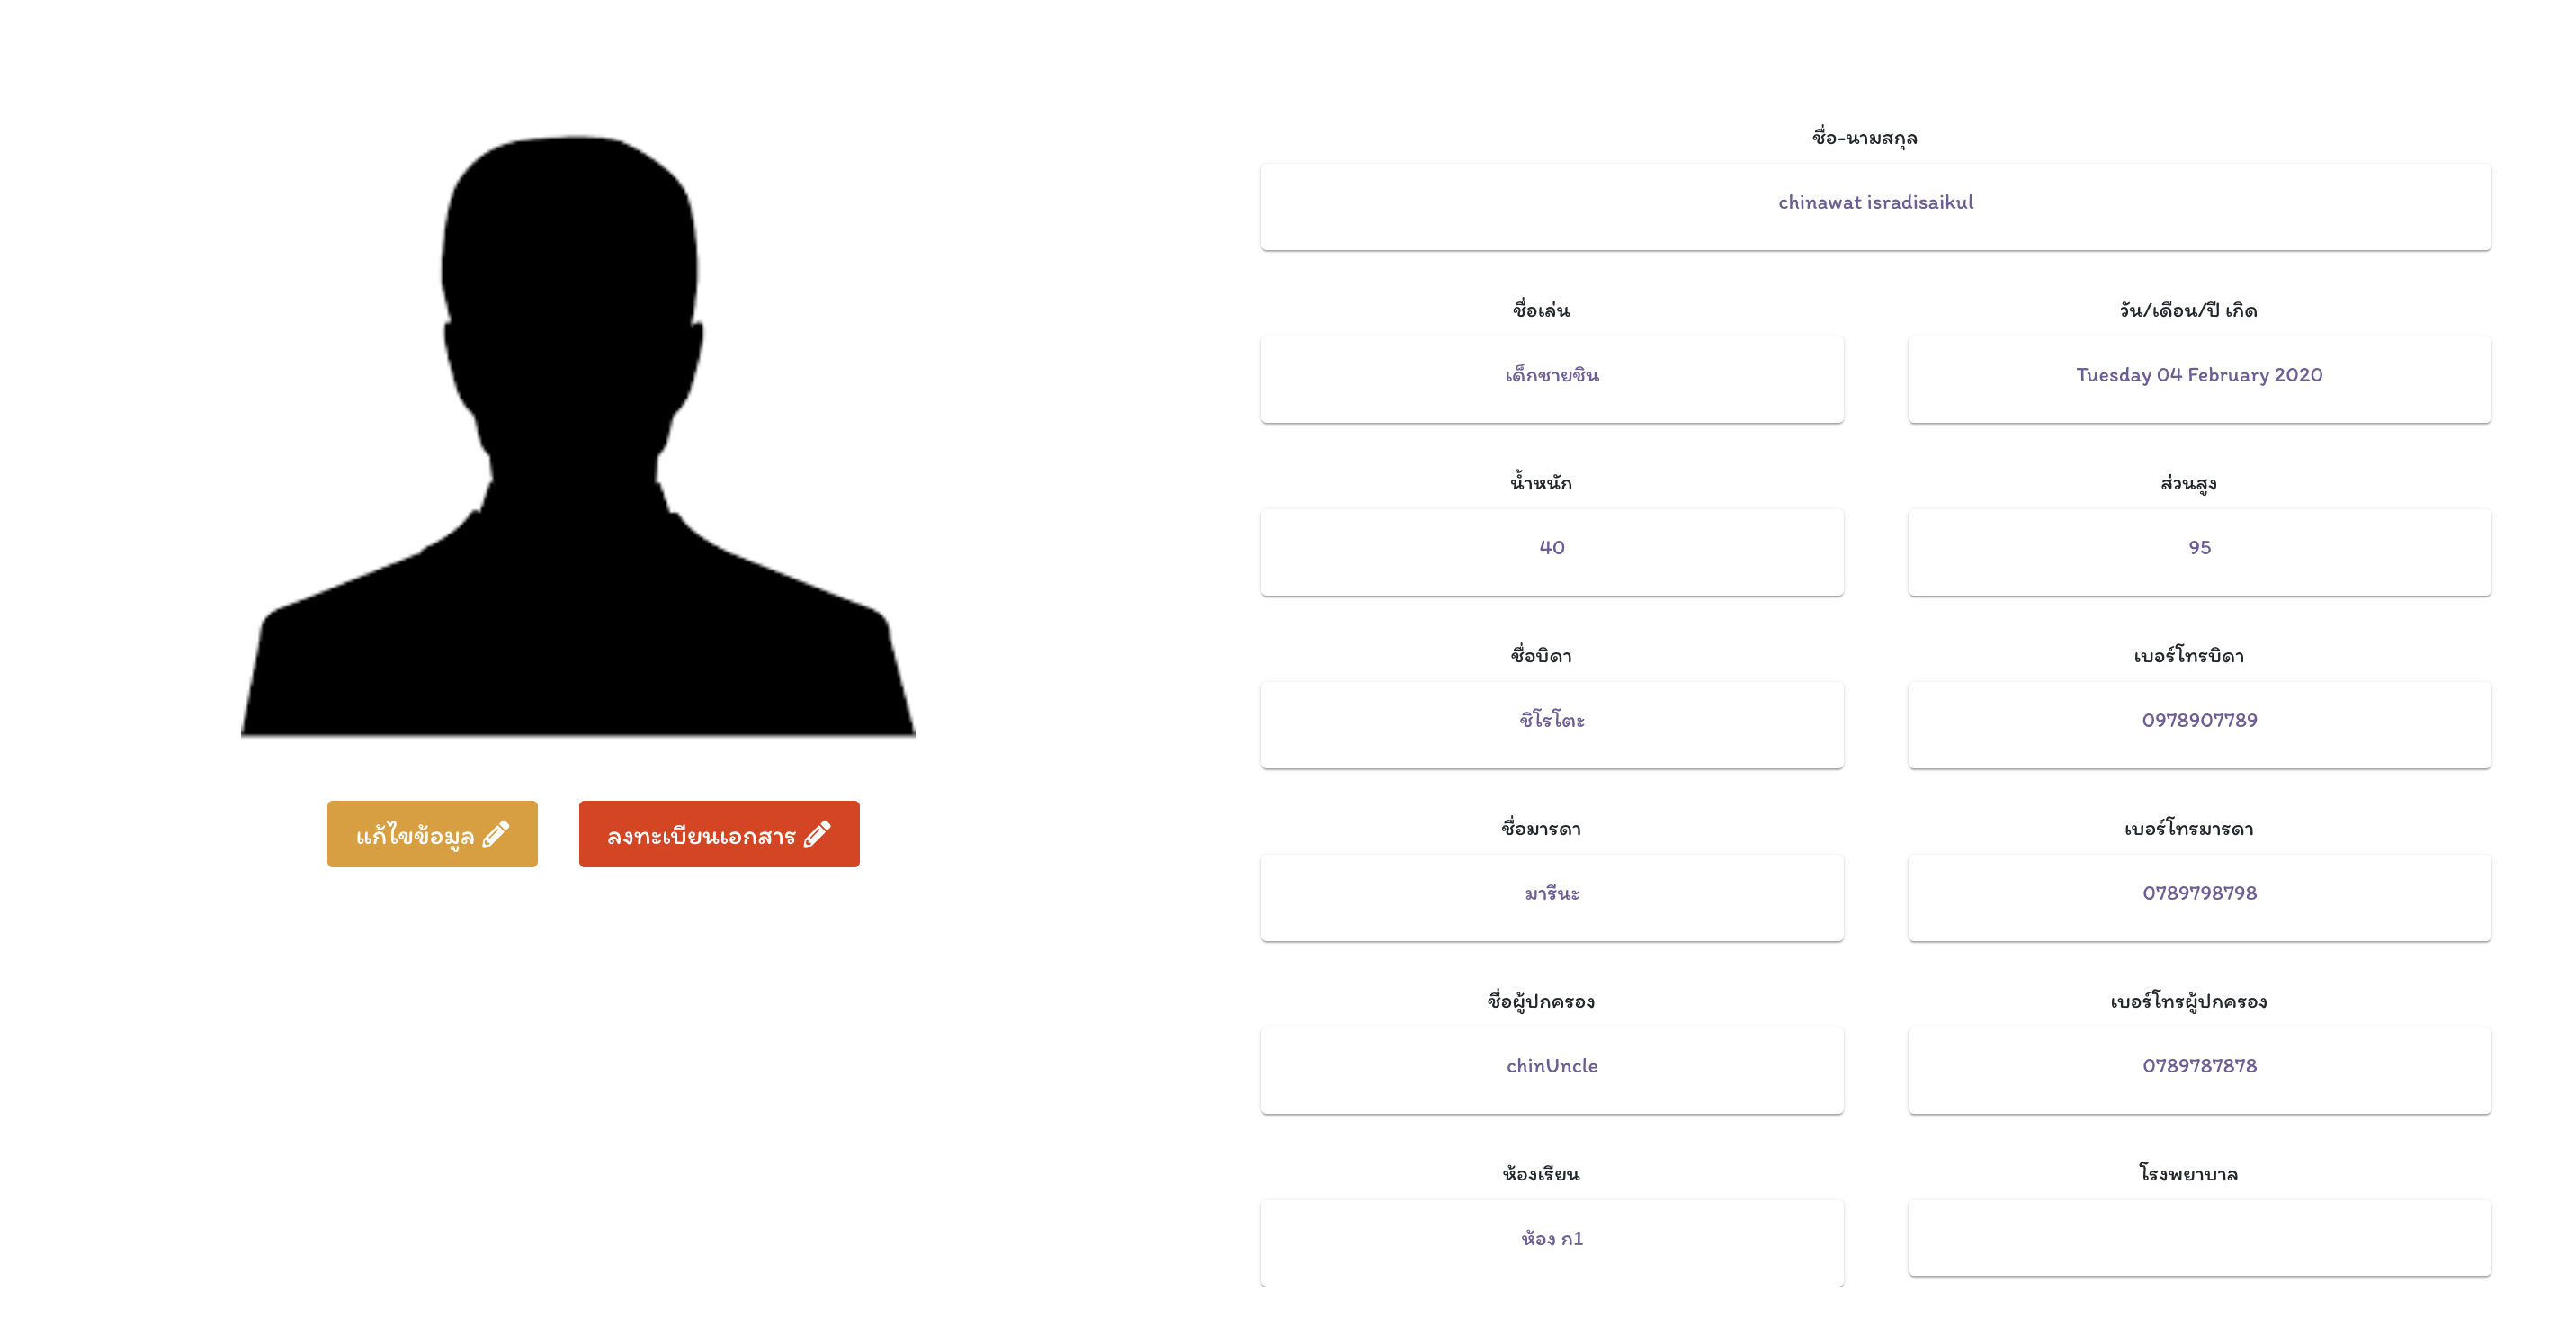
\includegraphics[width=\linewidth]{images/ProfileInfo.png}
      \end{center}
      \caption[หน้าประวัติส่วนตัวเด็ก]{หน้าประวัติส่วนตัวเด็ก}
      \label{fig:ProfileTwo}
    \end{figure}
  
  
    \begin{figure}
      \begin{center}
      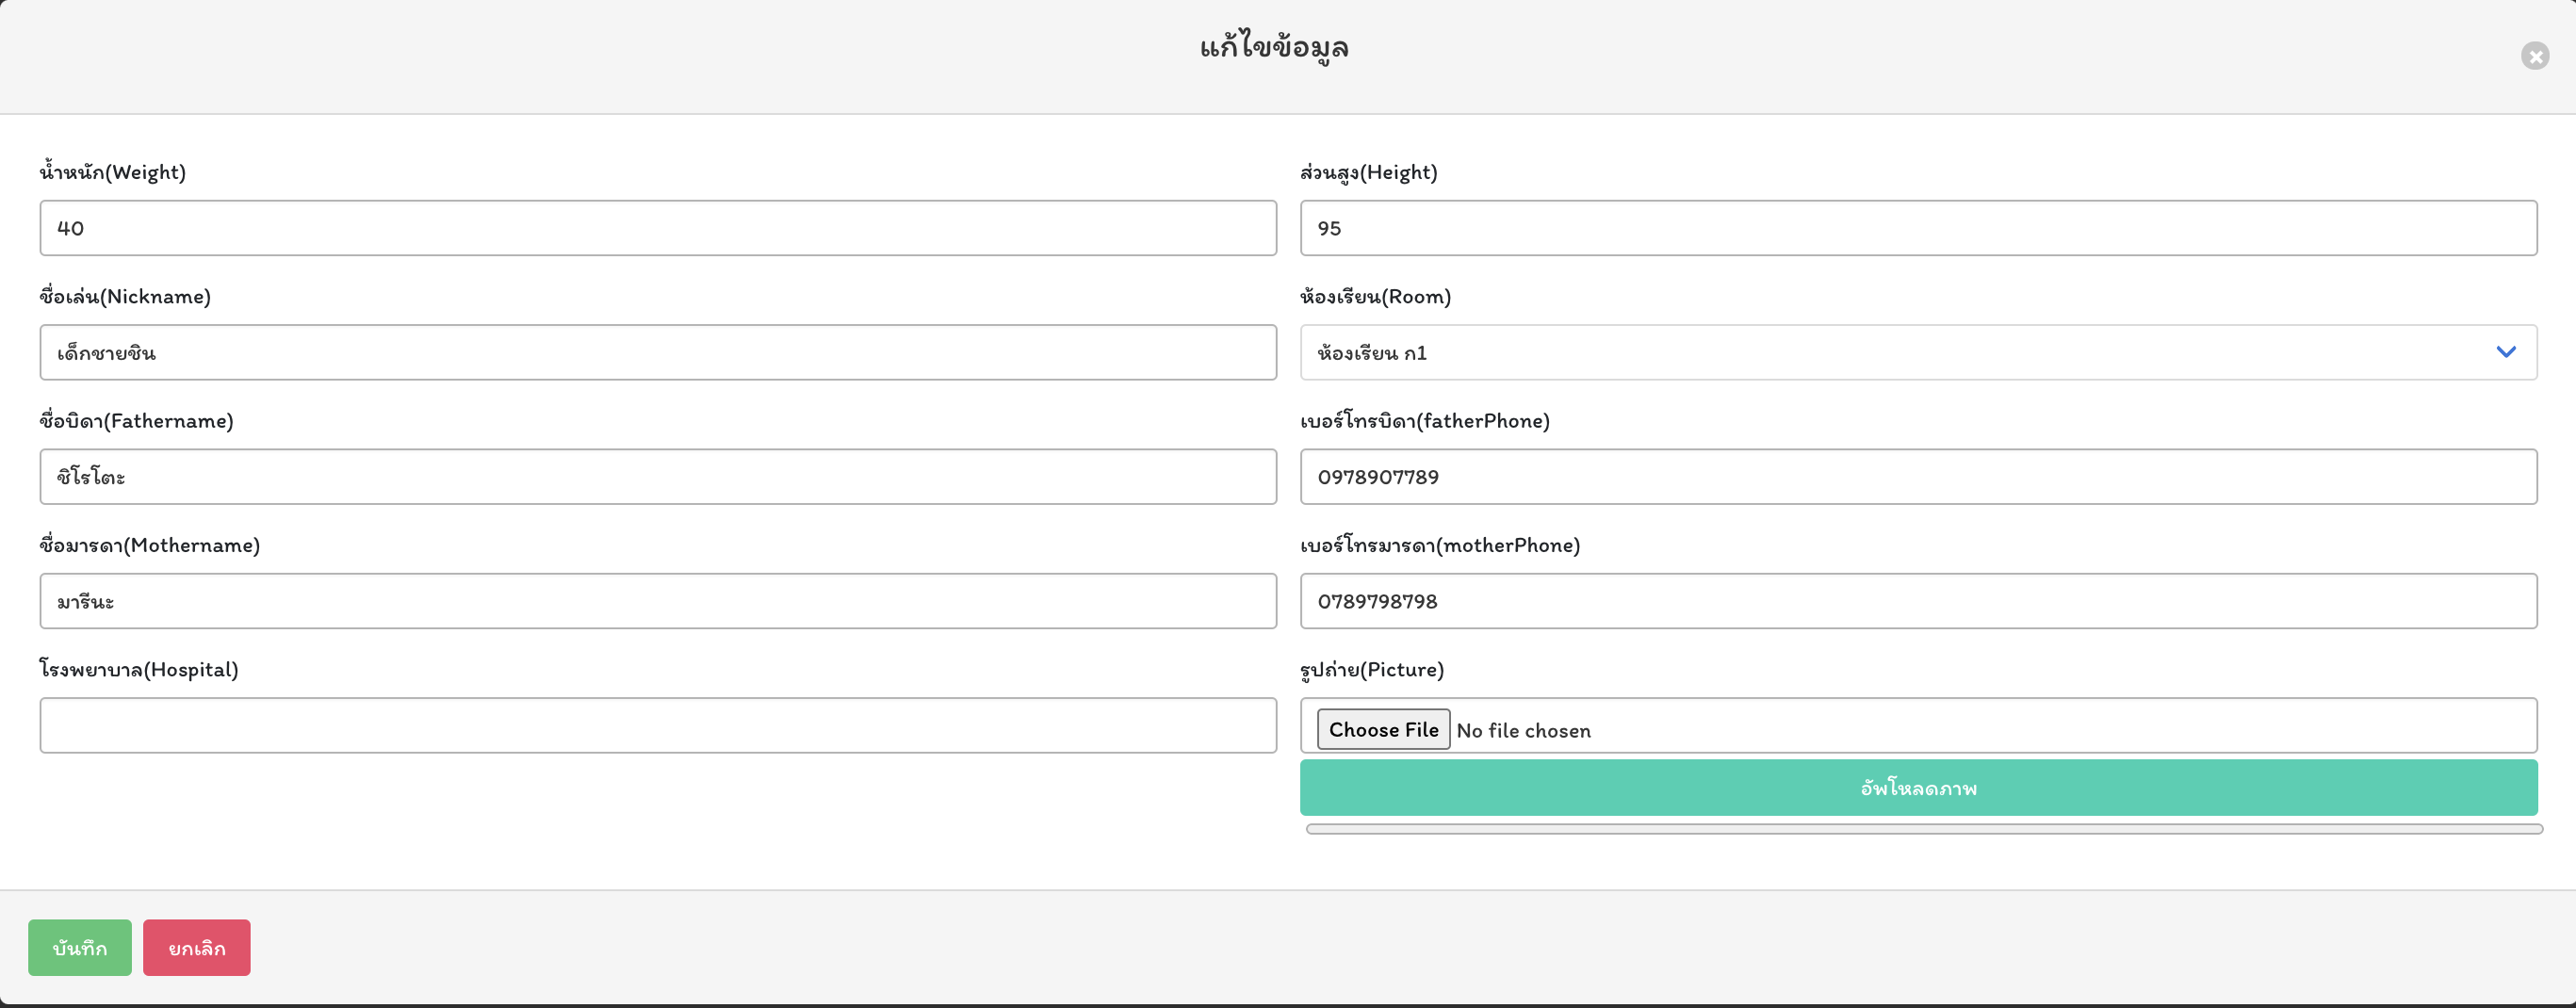
\includegraphics[width=\linewidth]{images/updateProfile.png}
      \end{center}
      \caption[หน้าแก้ไขข้อมูลเด็ก]{หน้าแก้ไขข้อมูลเด็ก}
      \label{fig:UpdateProfile}
      \end{figure}
  

  
    \begin{figure}
      \begin{center}
      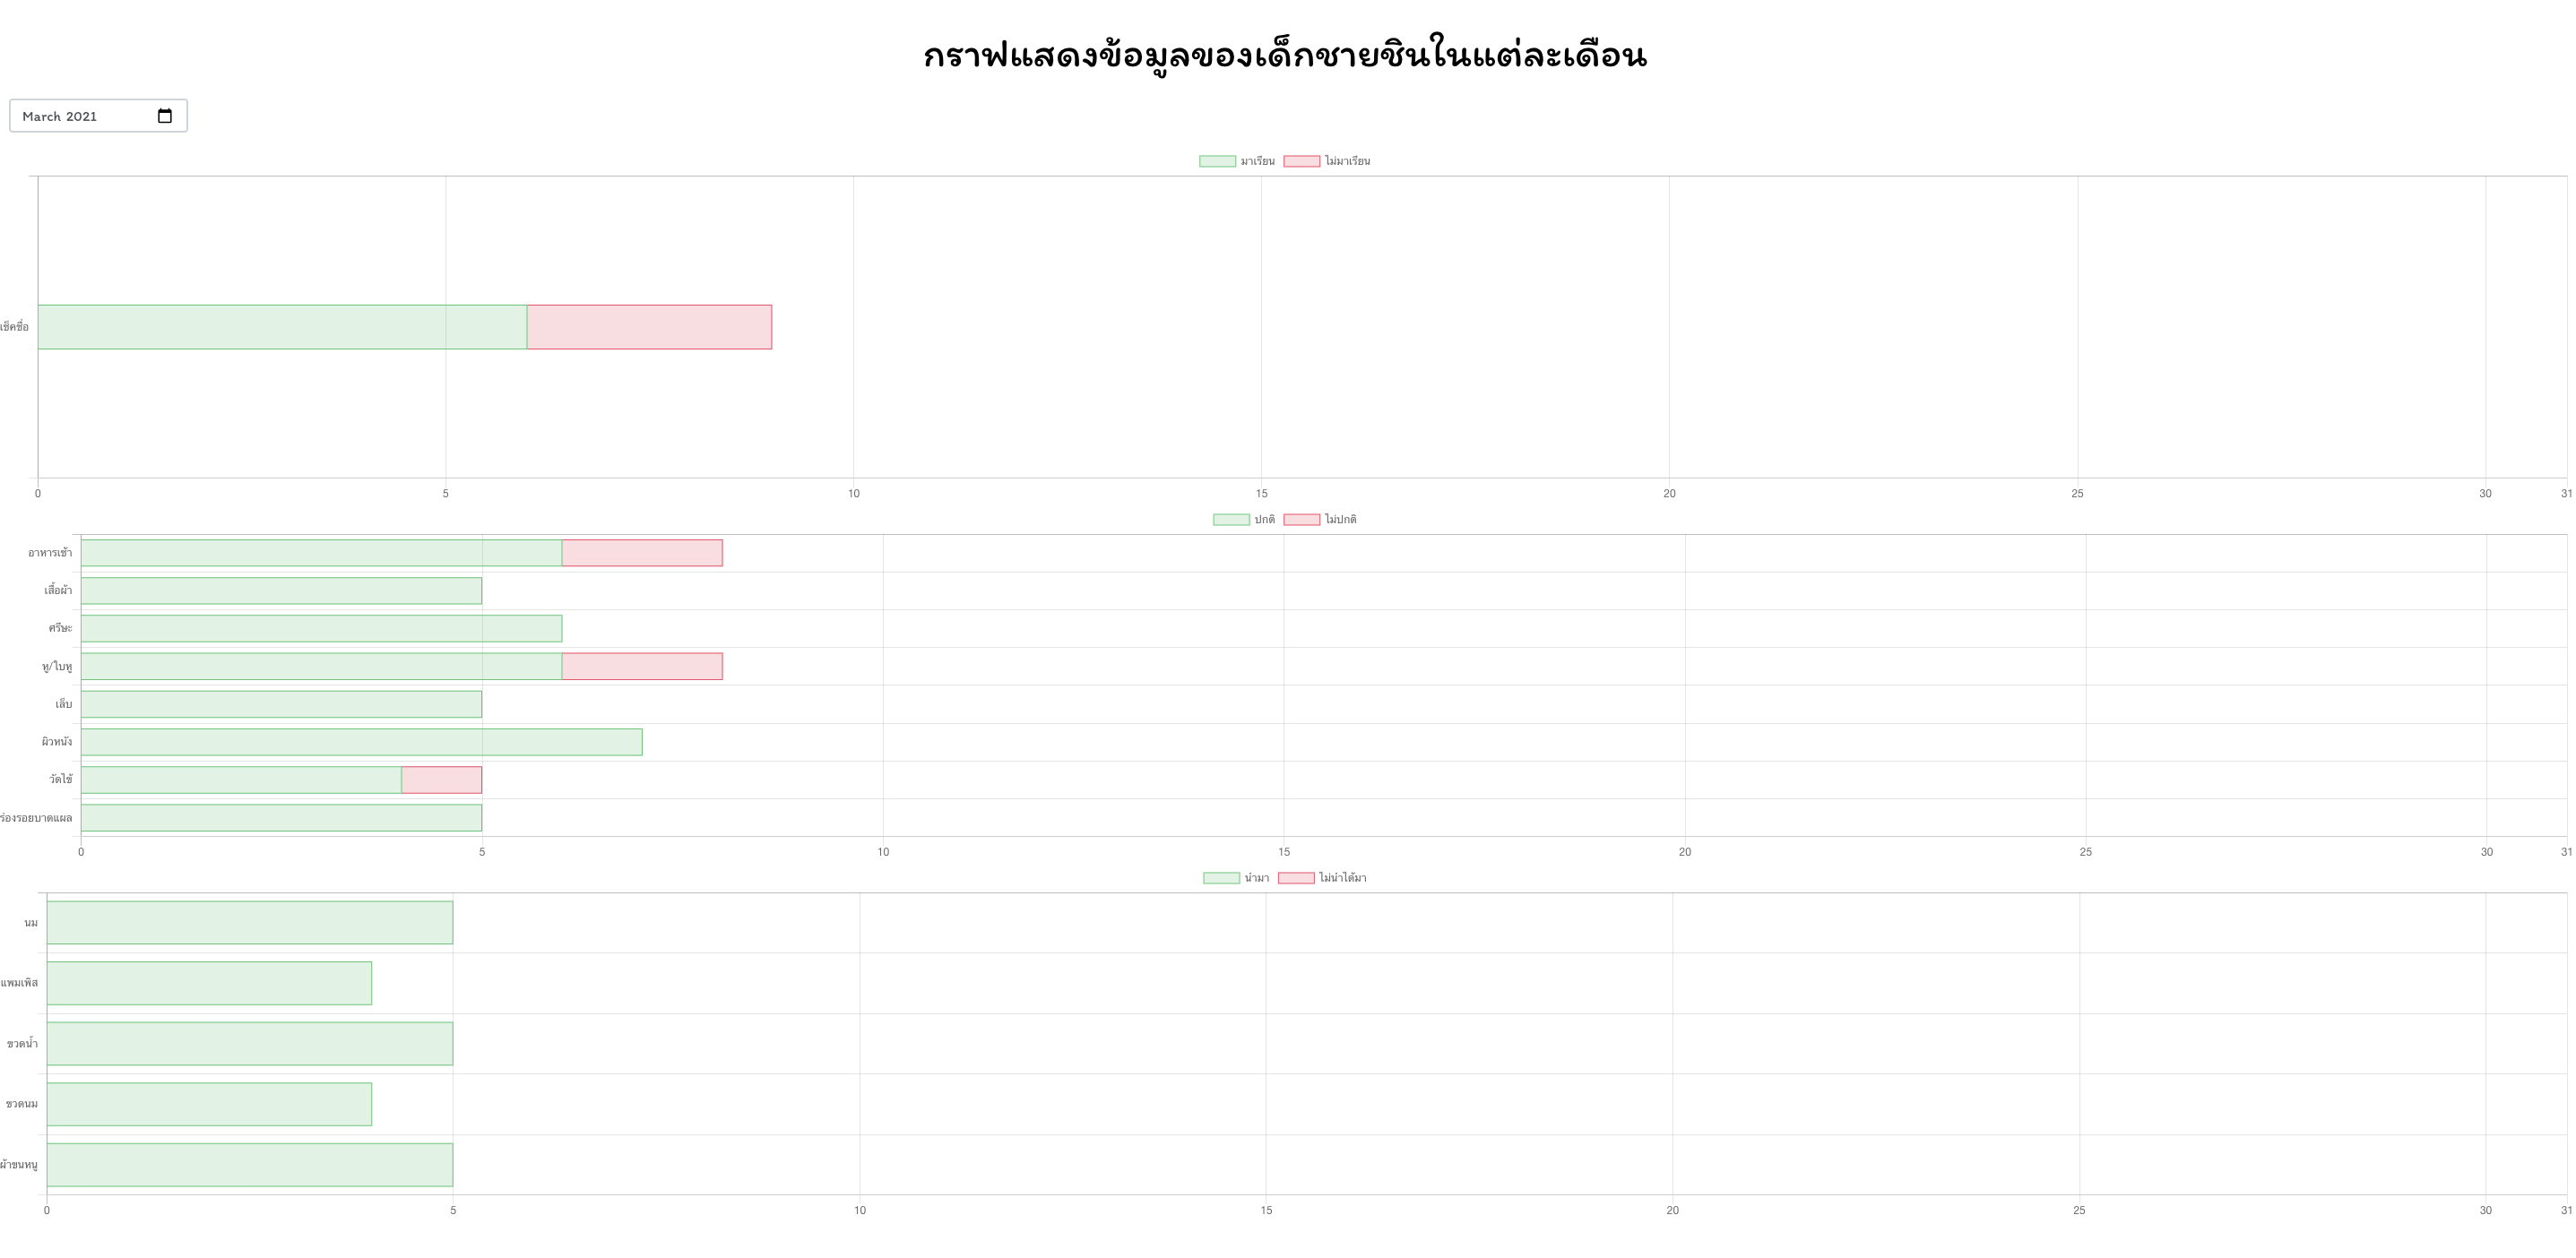
\includegraphics[width=\linewidth]{images/ChartPage.png}
      \end{center}
      \caption[หน้าแสดงข้อมูลรายเดือนเด็ก]{หน้าแสดงข้อมูลรายเดือนเด็ก}
      \label{fig:ChartPage}
    \end{figure}
  
  \item  Attendance คือ หน้าเช็คชื่อเด็กรายวัน ซึ่งหน้าแสดงผลหลักจะเป็นหน้านี้(รูปที่~\ref{fig:Attendance}) ซึ่งหน้าเช็คชื่อจะแสดงผลการเข้าเรียนของเด็กในเดือนและห้องทีผู้ใช้ได้เลือกไว้(ค่าเริ่มต้นจะเป็นเดือนปัจจุบันกับห้อง ก1) 
  โดยสามารถเลือกได้จากinputตรงมุมซ้ายบนล่าง menu bar ส่วนในการเช็คชื่อนั้น สามารถทำได้โดยกดปุ่มเช็คชื่อ
  จากนนั้นระบบจะนำผู้ใช้ไปยังหน้าเช็คชื่อ(รูป\ref{fig:CheckAttendance}) หน้านี้เป็นหน้าสำหรับให้ผู้ใช้เข้ามาเช็คข้อมูลเด็กในแต่ละวัน โดยมีวันที่ต้องการเช็คให้เลือกที่มุมขวาบน(ค่าเริ่มต้นจะเป็นวันปัจจุบัน)การเช็คชื่อทำได้ด้วยการกดที่ปุ่มด้านล่างสถานะกดหนึ่งครั้ง
  หน้าจะแสดงผลว่ามา กดอีกครั้งจะแสดงผลว่าไม่มา ถ้ากดอีกจะแสดงผลเป็นมา ไม่มา สลับกัน

  
    \begin{figure}
      \begin{center}
      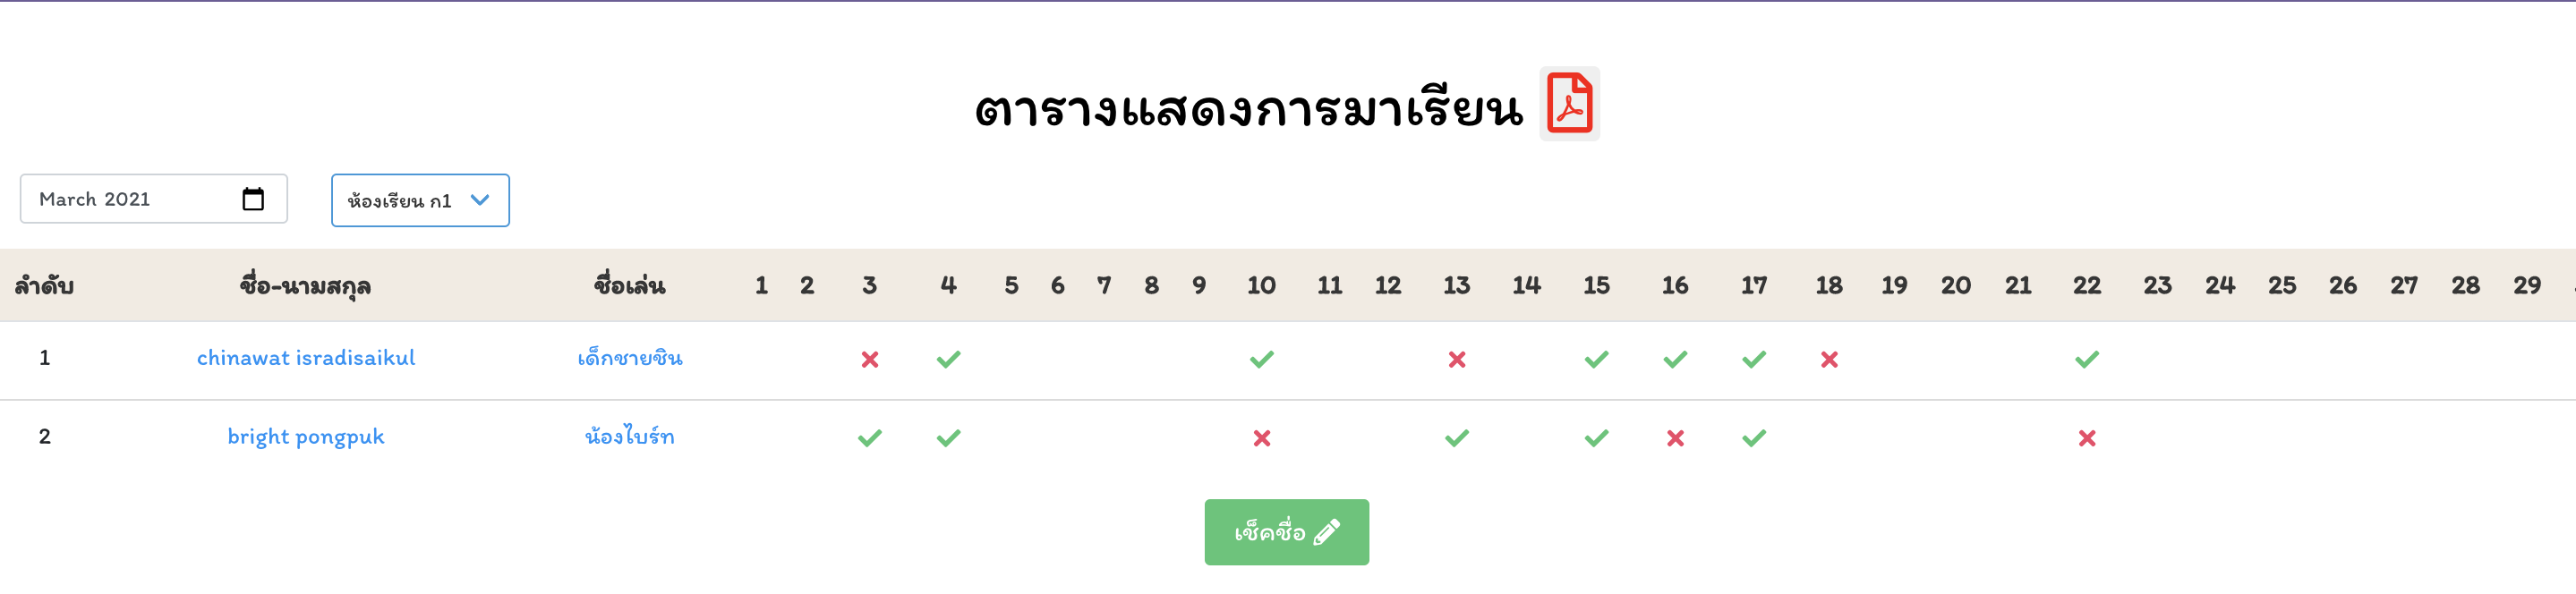
\includegraphics[width=\linewidth]{images/Attendance.png}
      \end{center}
      \caption[หน้าแสดงการเข้าเรียนเด็ก]{หน้าแสดงการเข้าเรียนเด็ก}
      \label{fig:Attendance}
    \end{figure}
  
  
  
    \begin{figure}
      \begin{center}
      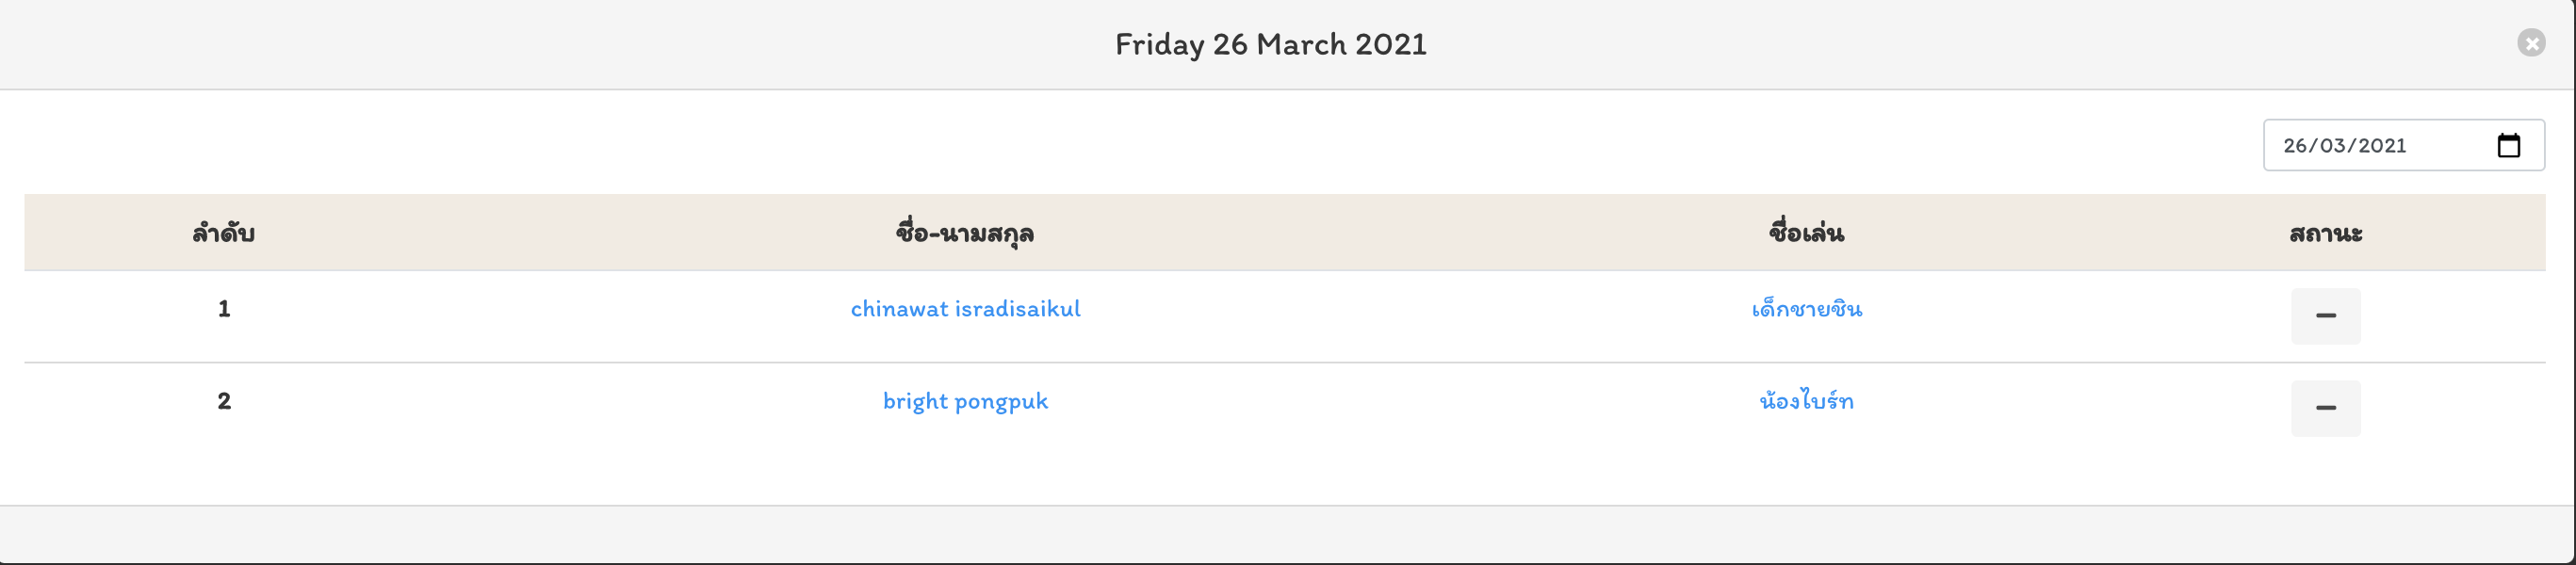
\includegraphics[width=\linewidth]{images/checkAttendance.png}
      \end{center}
      \caption[หน้าเช็คชื่อเด็ก]{หน้าเช็คชื่อเด็ก}
      \label{fig:CheckAttendance}
    \end{figure}
  

  \item  Health คือ หน้าเช็คสุขภาพเด็กรายวัน หน้านี้(รูป~\ref{fig:Health}) จะแสดงข้อมูลสุขภาพของเด็กรายวัน(ค่าเริ่มต้นจะเป็นวันปัจจุบันกับห้องเรียน ก1) โดยผู้ใช้สามารถเลือกวันและห้องเรียนที่ต้องการจะแสดงข้อมูลได้จากinputมุมซ้ายบนล่างmenu bar 
  หากผู้ใช้ต้องการเช็คข้อมูลให้กดปุ่มเช็คสุขภาพประจำวัน จากนั้นระบบจะนำผู้ใช้ไปยังหน้าเช็คสุขภาพประจำวัน (รูป~\ref{fig:CheckHealth}) 
  หน้านี้เป็นหน้าสำหรับให้ผู้ใช้เข้ามาเช็คข้อมูลเด็กในแต่ละวัน โดยที่การเช็คสุขภาพจะทำได้ด้วยการกดที่ปุ่มด้านล่างข้อมูลที่ต้องการเช็ค(อาหารเช้า, ศีรษะ, หู/ใบหู, เล็บ, ผิวหนัง, เสื้อผ้า, ร่องรอยบาดแผล, วัดไข้) กดหนึ่งครั้ง
  หน้าจะแสดงผลว่าปกติ กดอีกครั้งจะแสดงผลว่าไม่ปกติ ถ้ากดอีกจะแสดงผลเป็นปกติ ไม่ปกติ สลับกัน


    \begin{figure}
      \begin{center}
      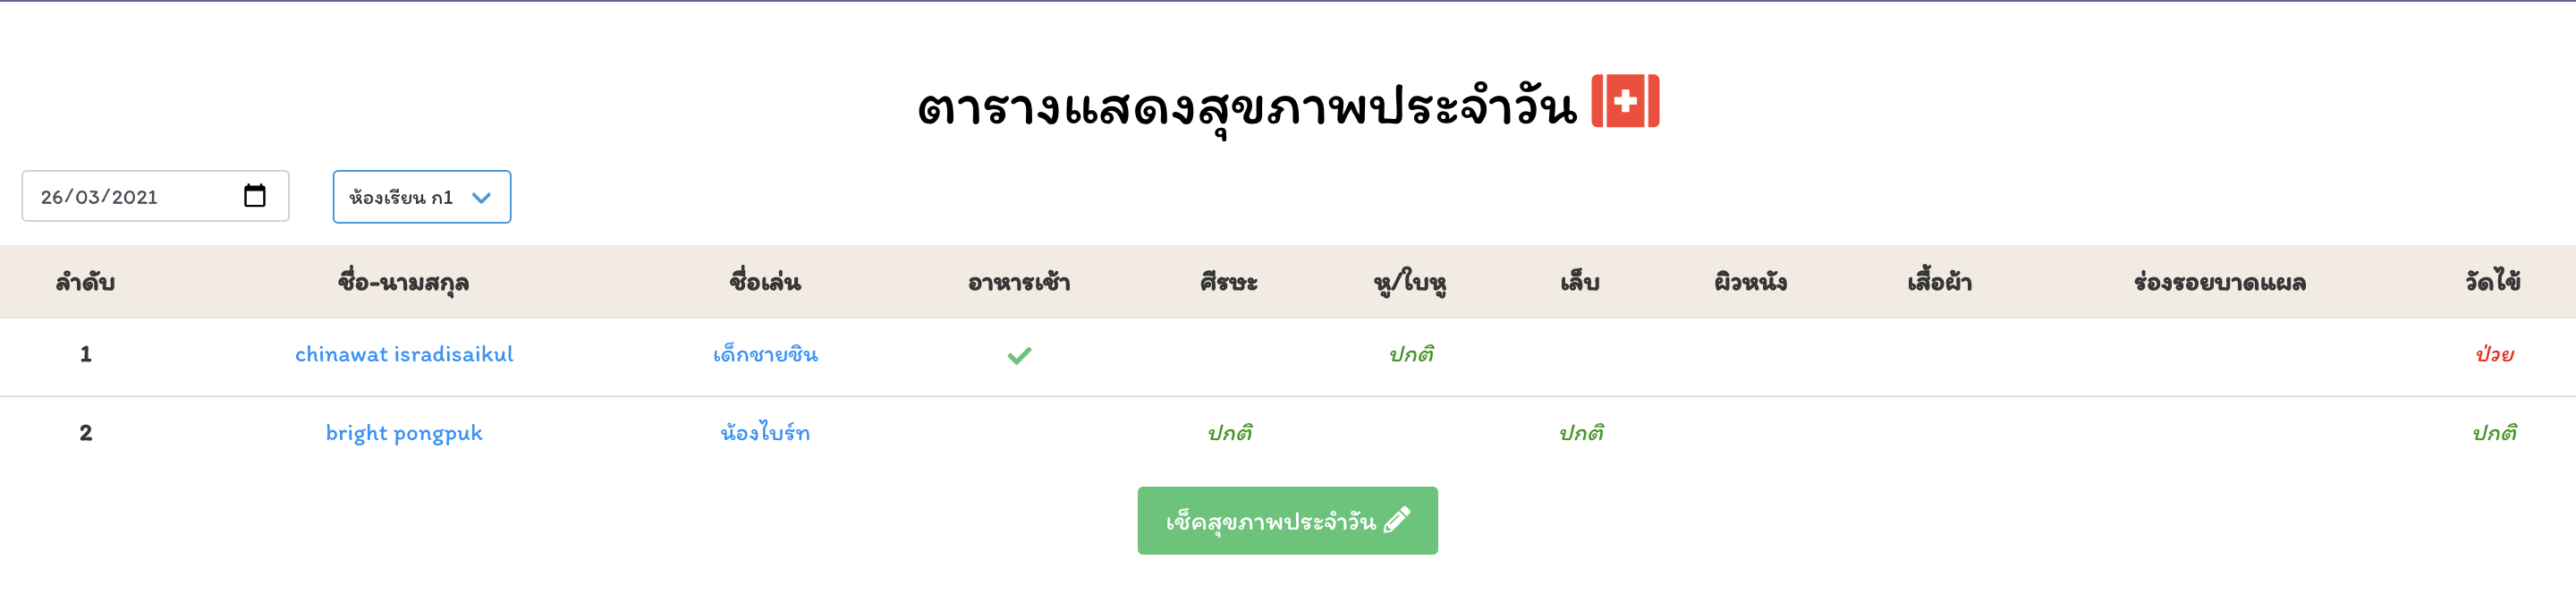
\includegraphics[width=\linewidth]{images/Health.png}
      \end{center}
      \caption[หน้าแสดงข้อมูลสุขภาพเด็กรายวัน]{หน้าแสดงข้อมูลสุขภาพเด็กรายวัน}
      \label{fig:Health}
      \end{figure}

    \begin{figure}
      \begin{center}
      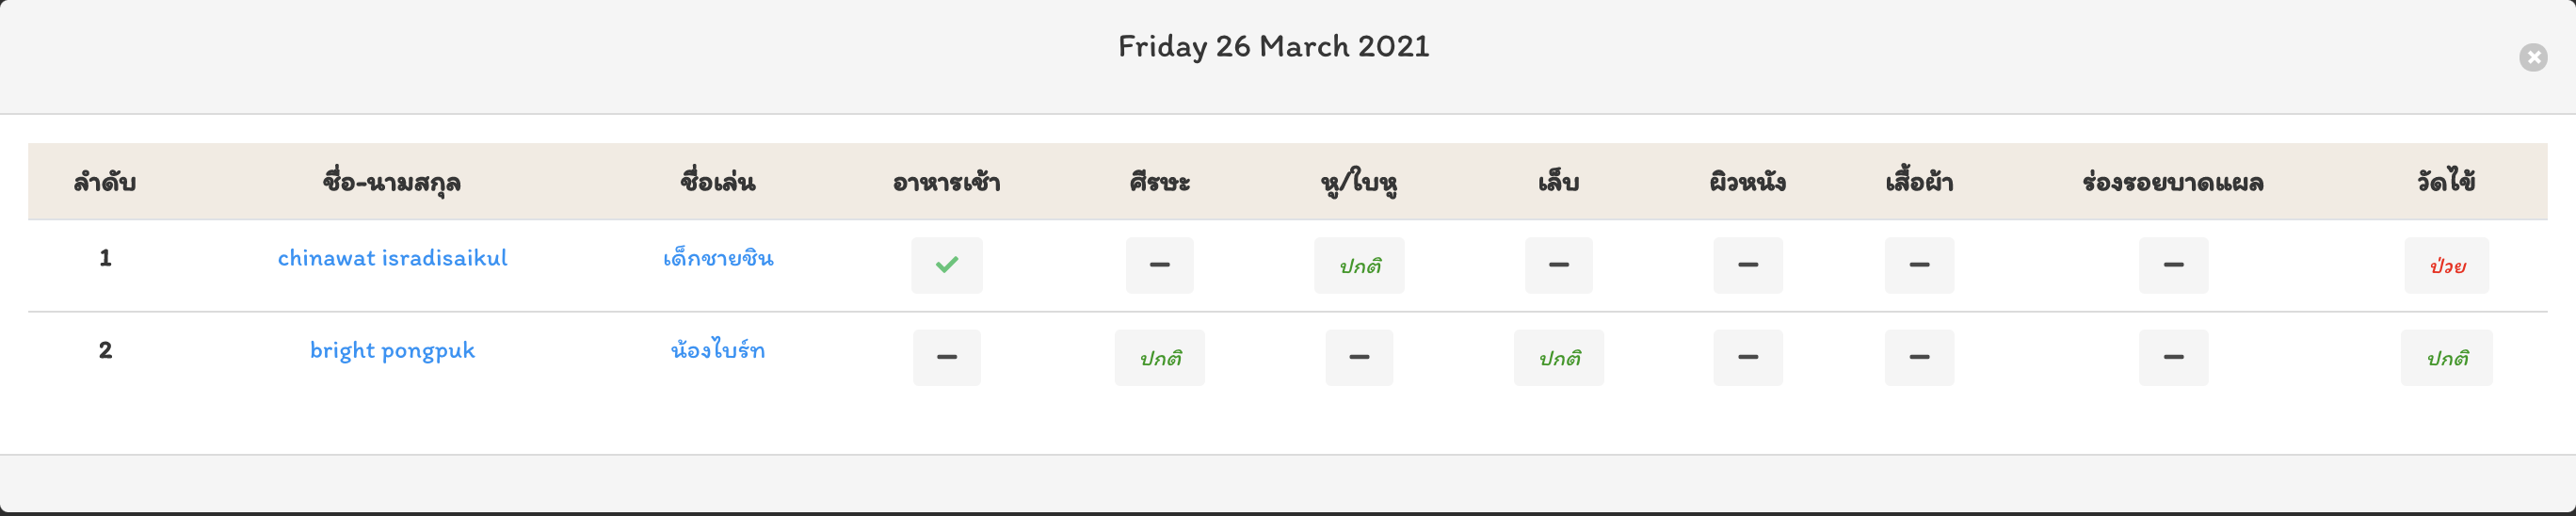
\includegraphics[width=\linewidth]{images/checkHealth.png}
      \end{center}
      \caption[หน้าเช็คสุขภาพเด็ก]{หน้าเช็คสุขภาพเด็ก}
      \label{fig:CheckHealth}
      \end{figure}

  \item  Gadget คือ หน้าเช็คอุปกรณ์เด็กรายวัน หน้านี้(รูปที่~\ref{fig:Gadget}) จะแสดงข้อมูลของที่เด็กเอามารายวัน(ค่าเริ่มต้นจะเป็นวันปัจจุบันกับห้องเรียน ก1) โดยผู้ใช้สามารถเลือกวันและห้องเรียนที่ต้องการจะแสดงข้อมูลได้จากinputมุมซ้ายบนล่างmenu bar 
  หากผู้ใช้ต้องการเช็คข้อมูลให้กดปุ่มเช็คอุปกรณ์ประจำวัน จากนั้นระบบจะนำผู้ใช้ไปยังหน้าเช็คอุปกรณ์ประจำวัน (รูป~\ref{fig:CheckGadget}) 
  หน้านี้เป็นหน้าสำหรับให้ผู้ใช้เข้ามาเช็คข้อมูลเด็กในแต่ละวัน โดยที่การเช็คอุปกรณ์จะทำได้ด้วยการกดที่ปุ่มด้านล่างข้อมูลที่ต้องการเช็ค(นม, แพมเพิส, ขวดน้ำ, ขวดนม, ผ้าขนหนู) กดหนึ่งครั้ง
  หน้าจะแสดงผลว่าเอามา(สัญลักษณ์เช็คถูก) กดอีกครั้งจะแสดงผลว่าไม่ได้เอามา(สัญลักษณ์เช็คผิด) ถ้ากดอีกจะแสดงผลเอามา ไม่เอามา สลับกัน
  \begin{figure}
    \begin{center}
    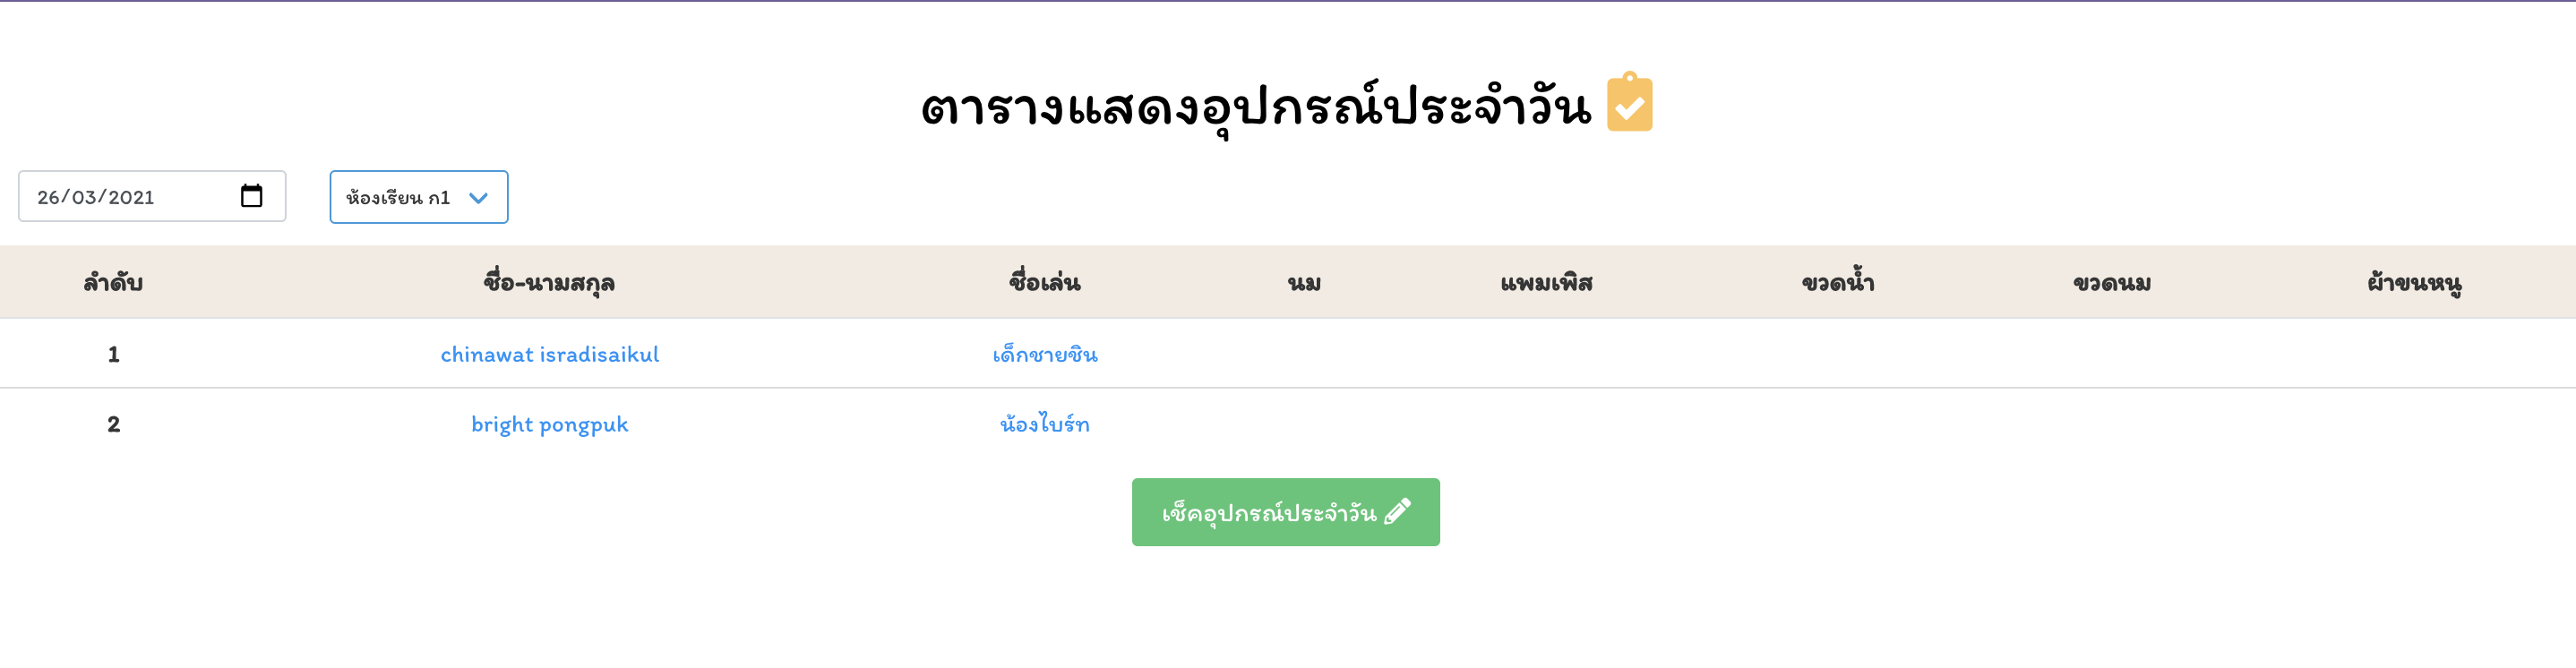
\includegraphics[width=\linewidth]{images/Gadget.png}
    \end{center}
    \caption[หน้าแสดงข้อมูลอุปกรณ์เด็กรายวัน]{หน้าแสดงข้อมูลอุปกรณ์เด็กรายวัน}
    \label{fig:Gadget}
    \end{figure}

  \begin{figure}
    \begin{center}
    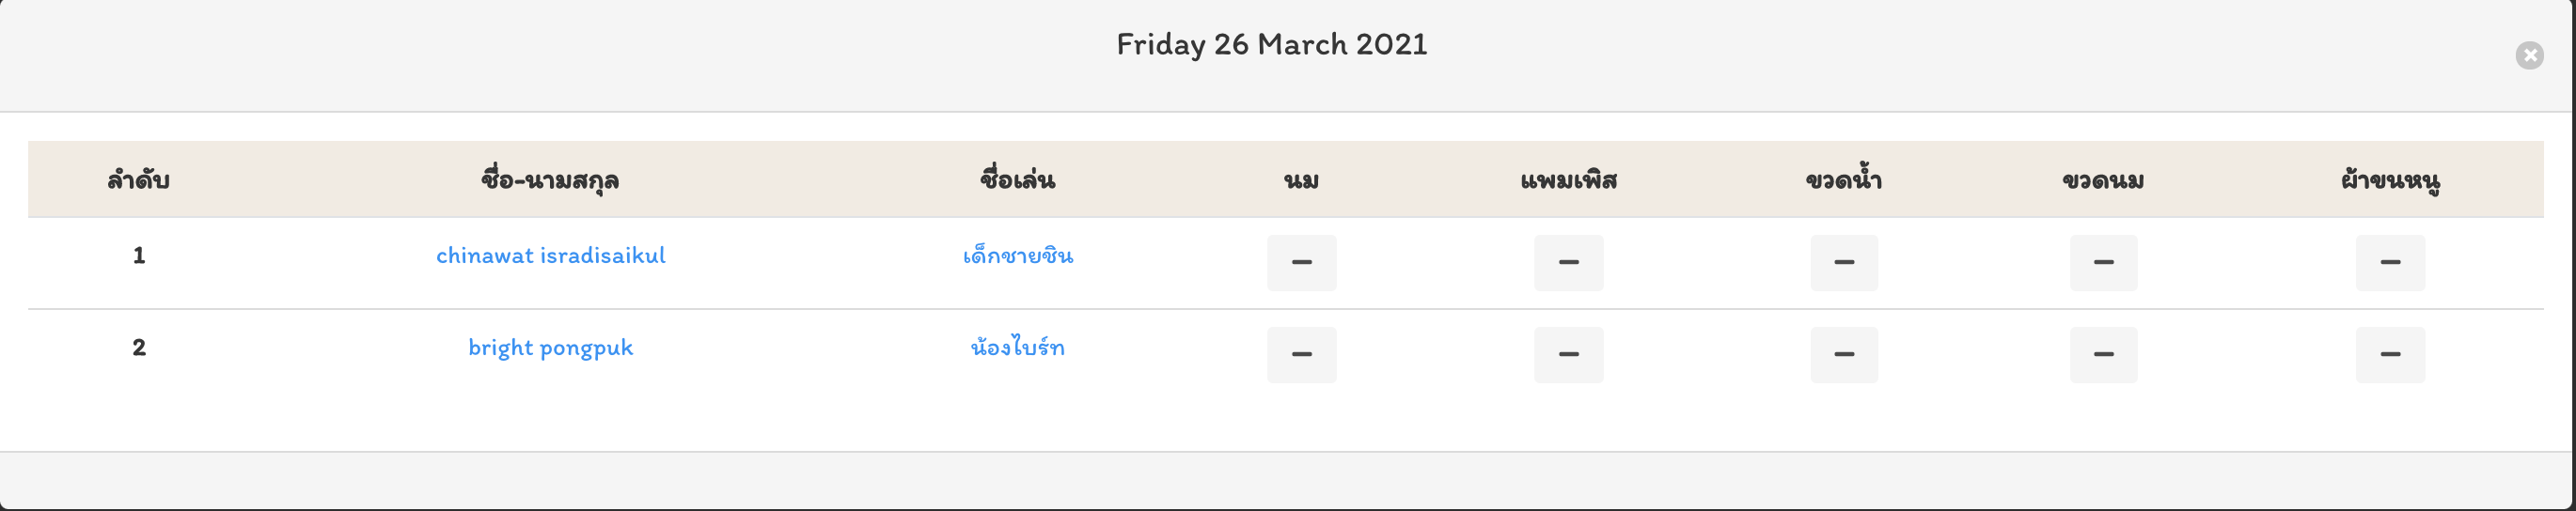
\includegraphics[width=\linewidth]{images/checkGadget.png}
    \end{center}
    \caption[หน้าเช็คอุปกรณ์เด็ก]{หน้าเช็คอุปกรณ์เด็ก}
    \label{fig:CheckGadget}
    \end{figure}
  \item  Stock คือ หน้าจัดการคลังสินค้าใน nursery โดยที่มีหน้านี้เป็นหน้าหลักของการทำงานระบบคลังสินค้า(รูปที่~\ref{fig:Stock}) โดยที่หน้าคลังสินค้าหลักจะแสดงข้อมูลของที่ทาง nursery มีว่ามีจำนวนทั้งหมดกี่ชิ้น มีของอะไรบ้าง และหน้านี้จะมีปุ่มให้เลือกใช้
  อยู่สามปุ่มหลัก คือ ปุ่มประวัติ, ปุ่มราคาของในคลัง, แก้ไข 
  
  ซึ่งปุ่มประวัติเมื่อคลิกระบบจะนำผู้ใช้ไปยังหน้าแสดงประวัติการจัดการstockของ(รูป~\ref{fig:HistoryStock}) หน้านี้จะแสดงข้อมูลว่าของชิ้นไหน ขนาดอะไร จำนวนกี่ชิ้น ที่มีการเปลี่ยนแปลง(เพิ่ม,ลด) และ แสดงวันที่มีการเข้ามาแก้ไข แก้ไขโดยใคร
  
  ส่วนปุ่มราคาของในคลังสินค้า(รูป~\ref{fig:editPrice}) จะแสดงข้อมูลราคาของใน nursery (ค่าเริ่มต้นจะเป็นไซส์ S) สามารถเลือกไซส์ที่ต้องการดูข้อมูลด้วยการ เลือกจากinputทางด้านขวาบน ในส่วนของการแก้ไขราคาสามารถทำได้ด้วย การกดปุ่มปากกาสีฟ้า จากนั้นก็กรอกค่าที่ต้องการเปลี่ยน
  จากนั้นกดยืนยันเป็นอันเสร็จสิ้น
  
  ส่วนแก้ไข(รูป~\ref{fig:CheckStock}) จะแสดงข้อมูลจำนวนของใน nursery (ค่าเริ่มต้นจะเป็นไซส์ S) สามารถเลือกไซส์ที่ต้องการดูข้อมูลด้วยการ เลือกจากinputทางด้านขวาบน ในส่วนของการแก้ไขจำนวนสามารถทำได้ด้วย การกดปุ่มบวกหรือลบตามที่ผู้ใช้ต้องการ หากต้องการเพิ่มของให้กดบวก จากนั้นก็กรอกค่าที่ต้องการเพิ่ม
  โดยค่าที่กรอกจะไปบวกเพิ่มกับค่าเก่าที่แสดงให้เห็นกดหน้าที่จะกดบวก ในส่วนของการลดจำนวนของให้กดที่ปุ่มลบ จากนั้นก็กรอกค่าที่ต้องการลด โดยค่าที่กรอกจะไปลบกับค่าเก่าที่แสดงให้เห็นกดหน้าที่จะกดลบ จากนั้นกดยืนยันเป็นอันเสร็จสิ้น

  
    \begin{figure}
      \begin{center}
      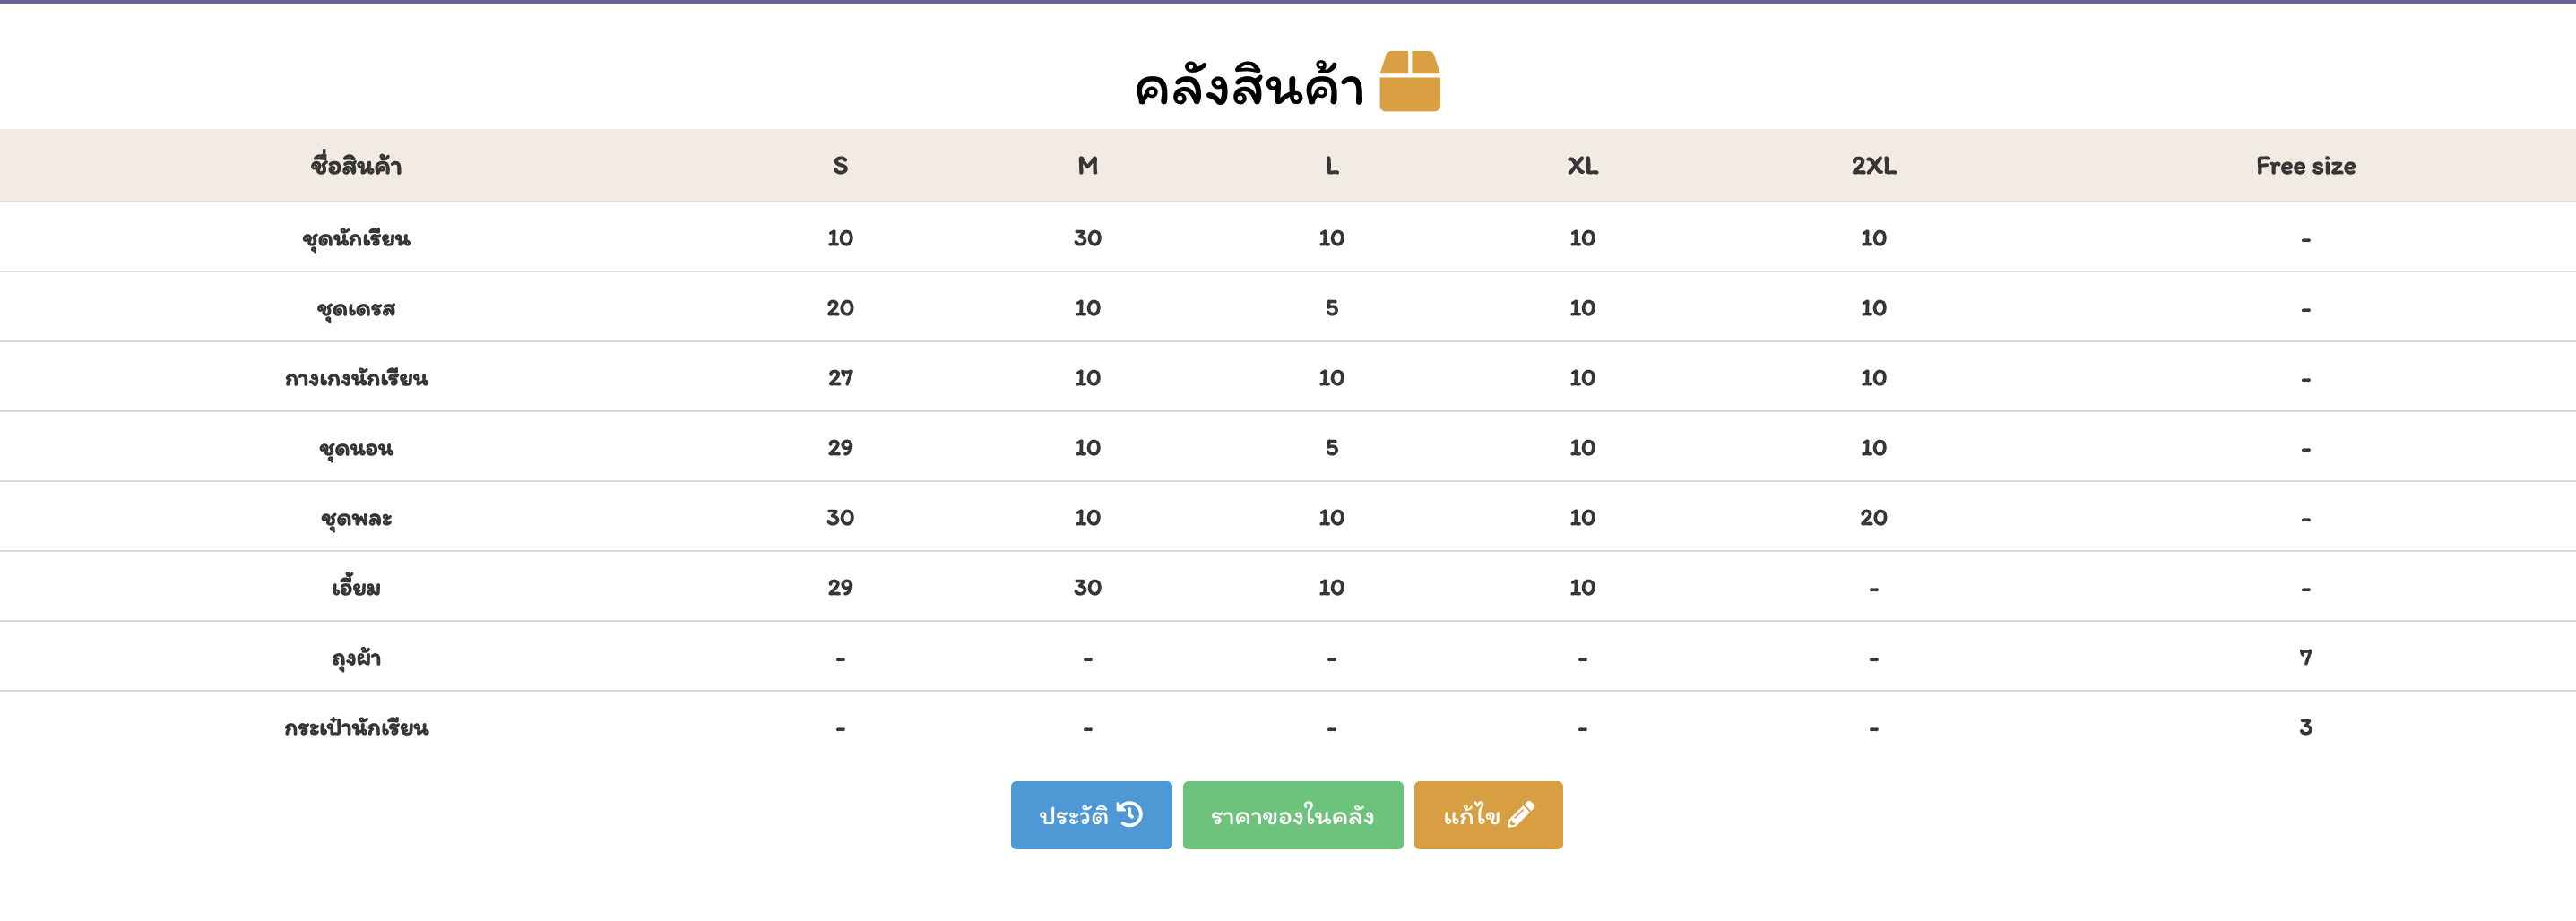
\includegraphics[width=\linewidth]{images/Stock.png}
      \end{center}
      \caption[หน้าแสดงคลังสินค้า]{หน้าแสดงคลังสินค้า}
      \label{fig:Stock}
      \end{figure}
  
  
    \begin{figure}
      \begin{center}
      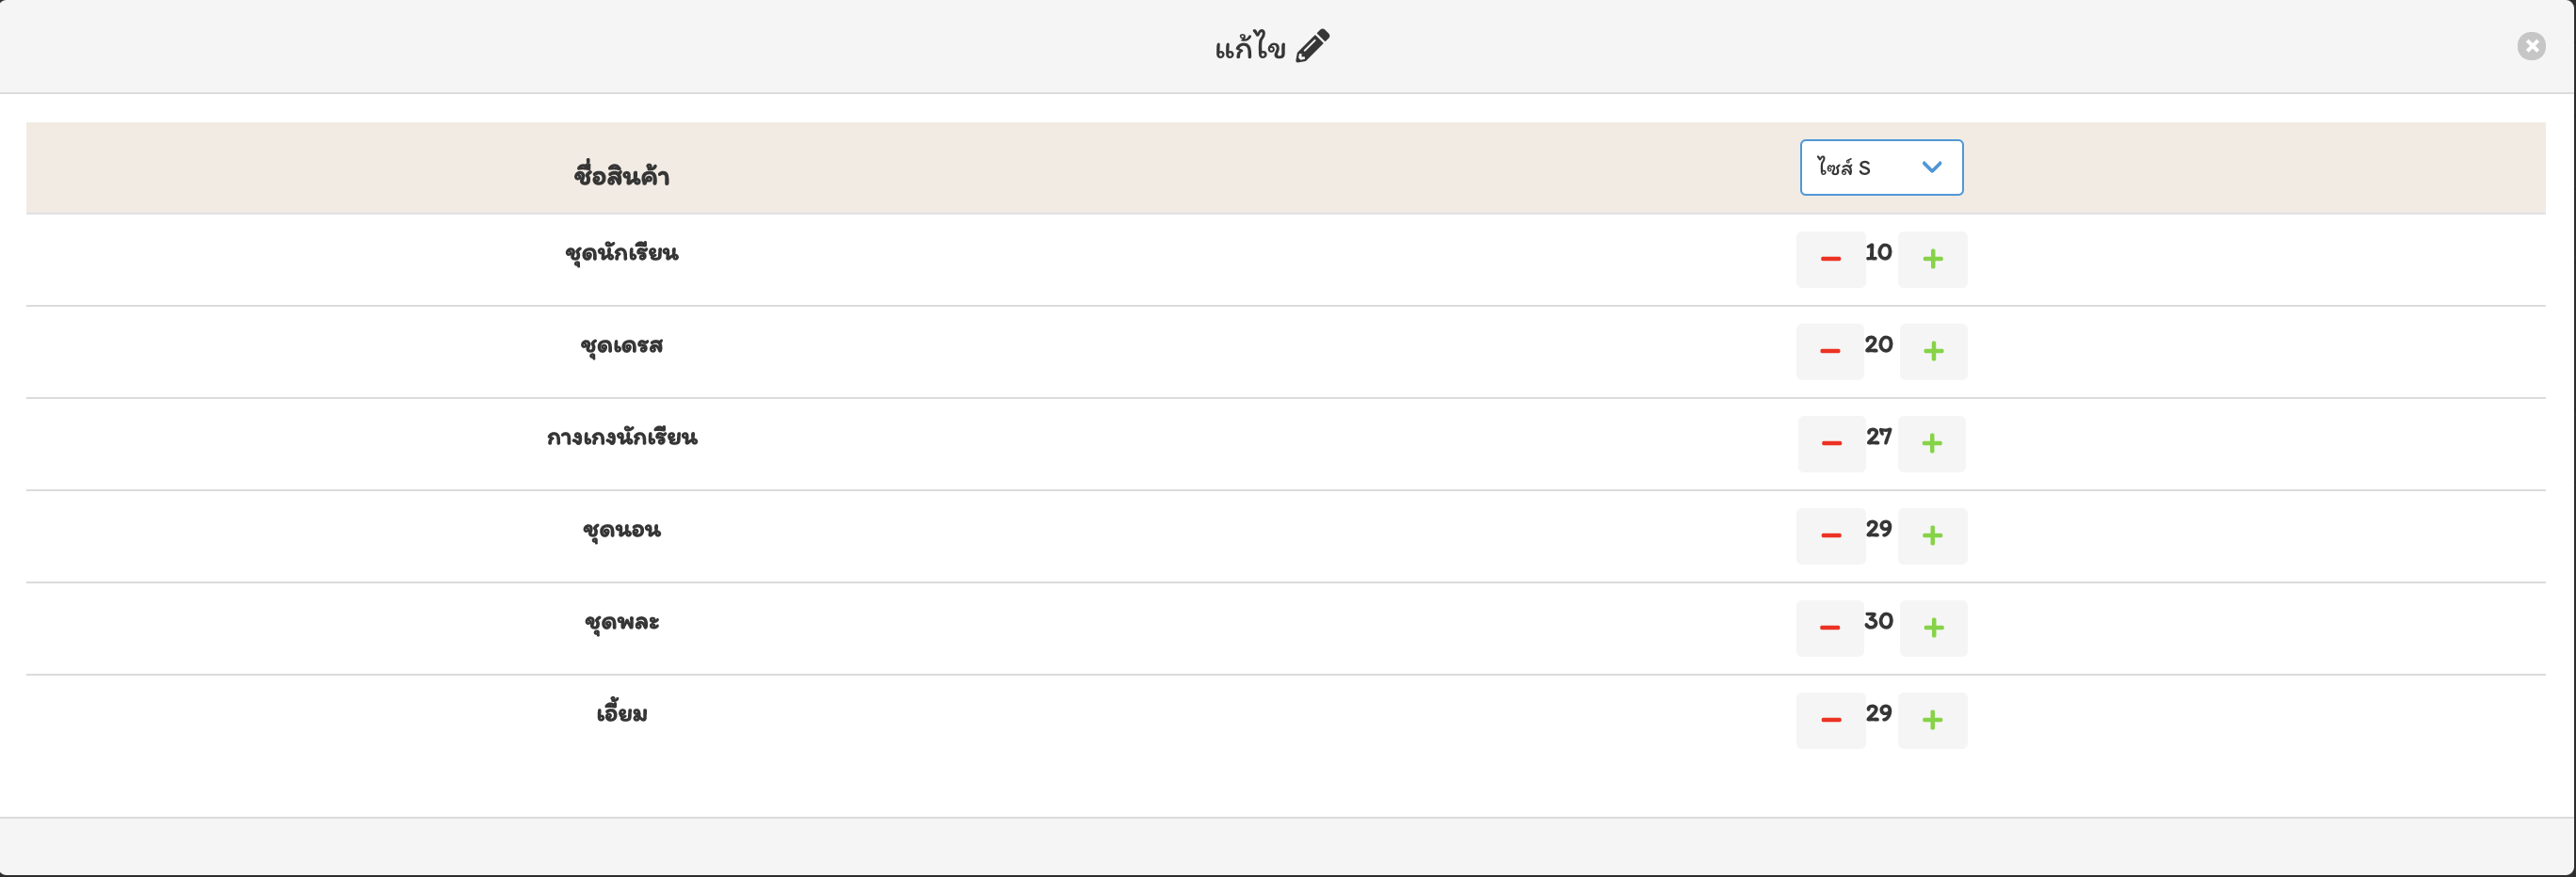
\includegraphics[width=\linewidth]{images/handleStock.png}
      \end{center}
      \caption[หน้าจัดการแก้ไขสต็อกของ]{หน้าจัดการแก้ไขสต็อกของ}
      \label{fig:CheckStock}
      \end{figure}
  
  
  
    \begin{figure}
      \begin{center}
      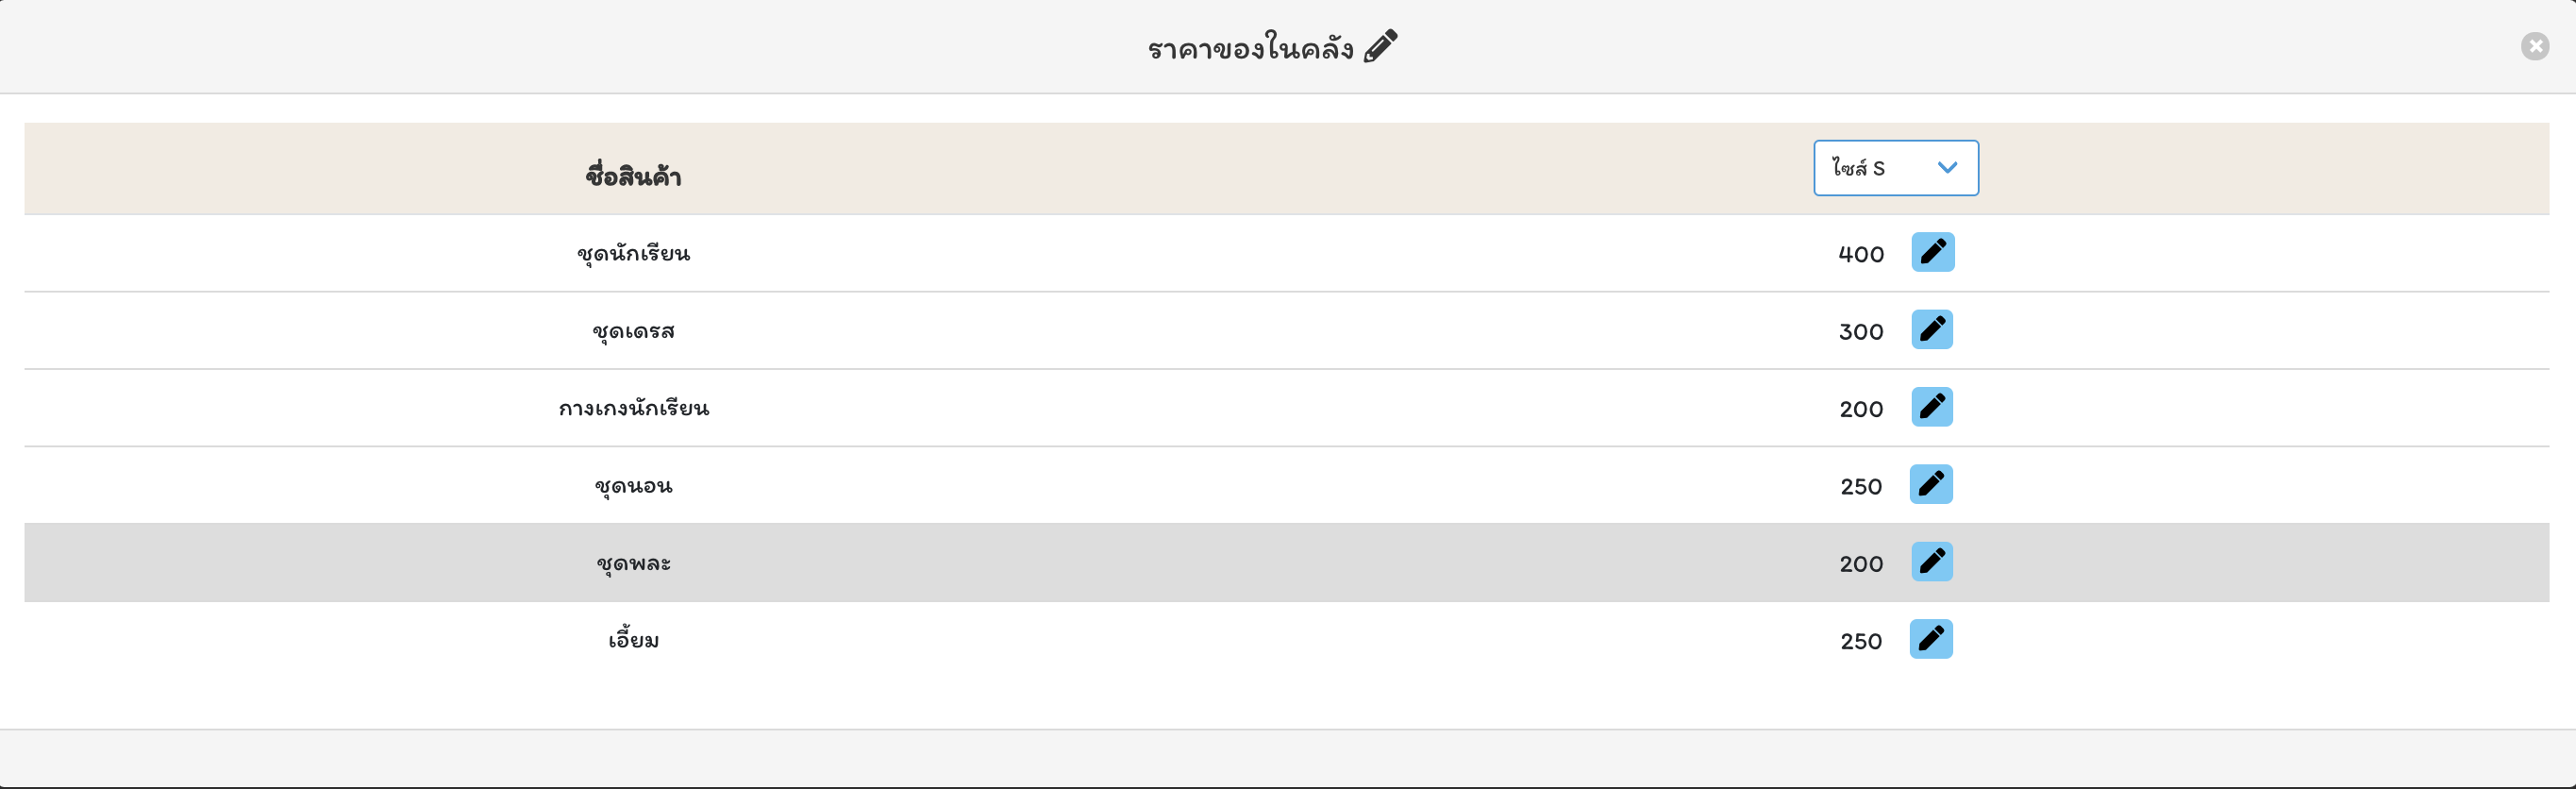
\includegraphics[width=\linewidth]{images/editPrice.png}
      \end{center}
      \caption[หน้าจัดการแก้ไขราคาสินค้า]{หน้าจัดการแก้ไขราคาสินค้า}
      \label{fig:editPrice}
      \end{figure}
  
  
    \begin{figure}
      \begin{center}
      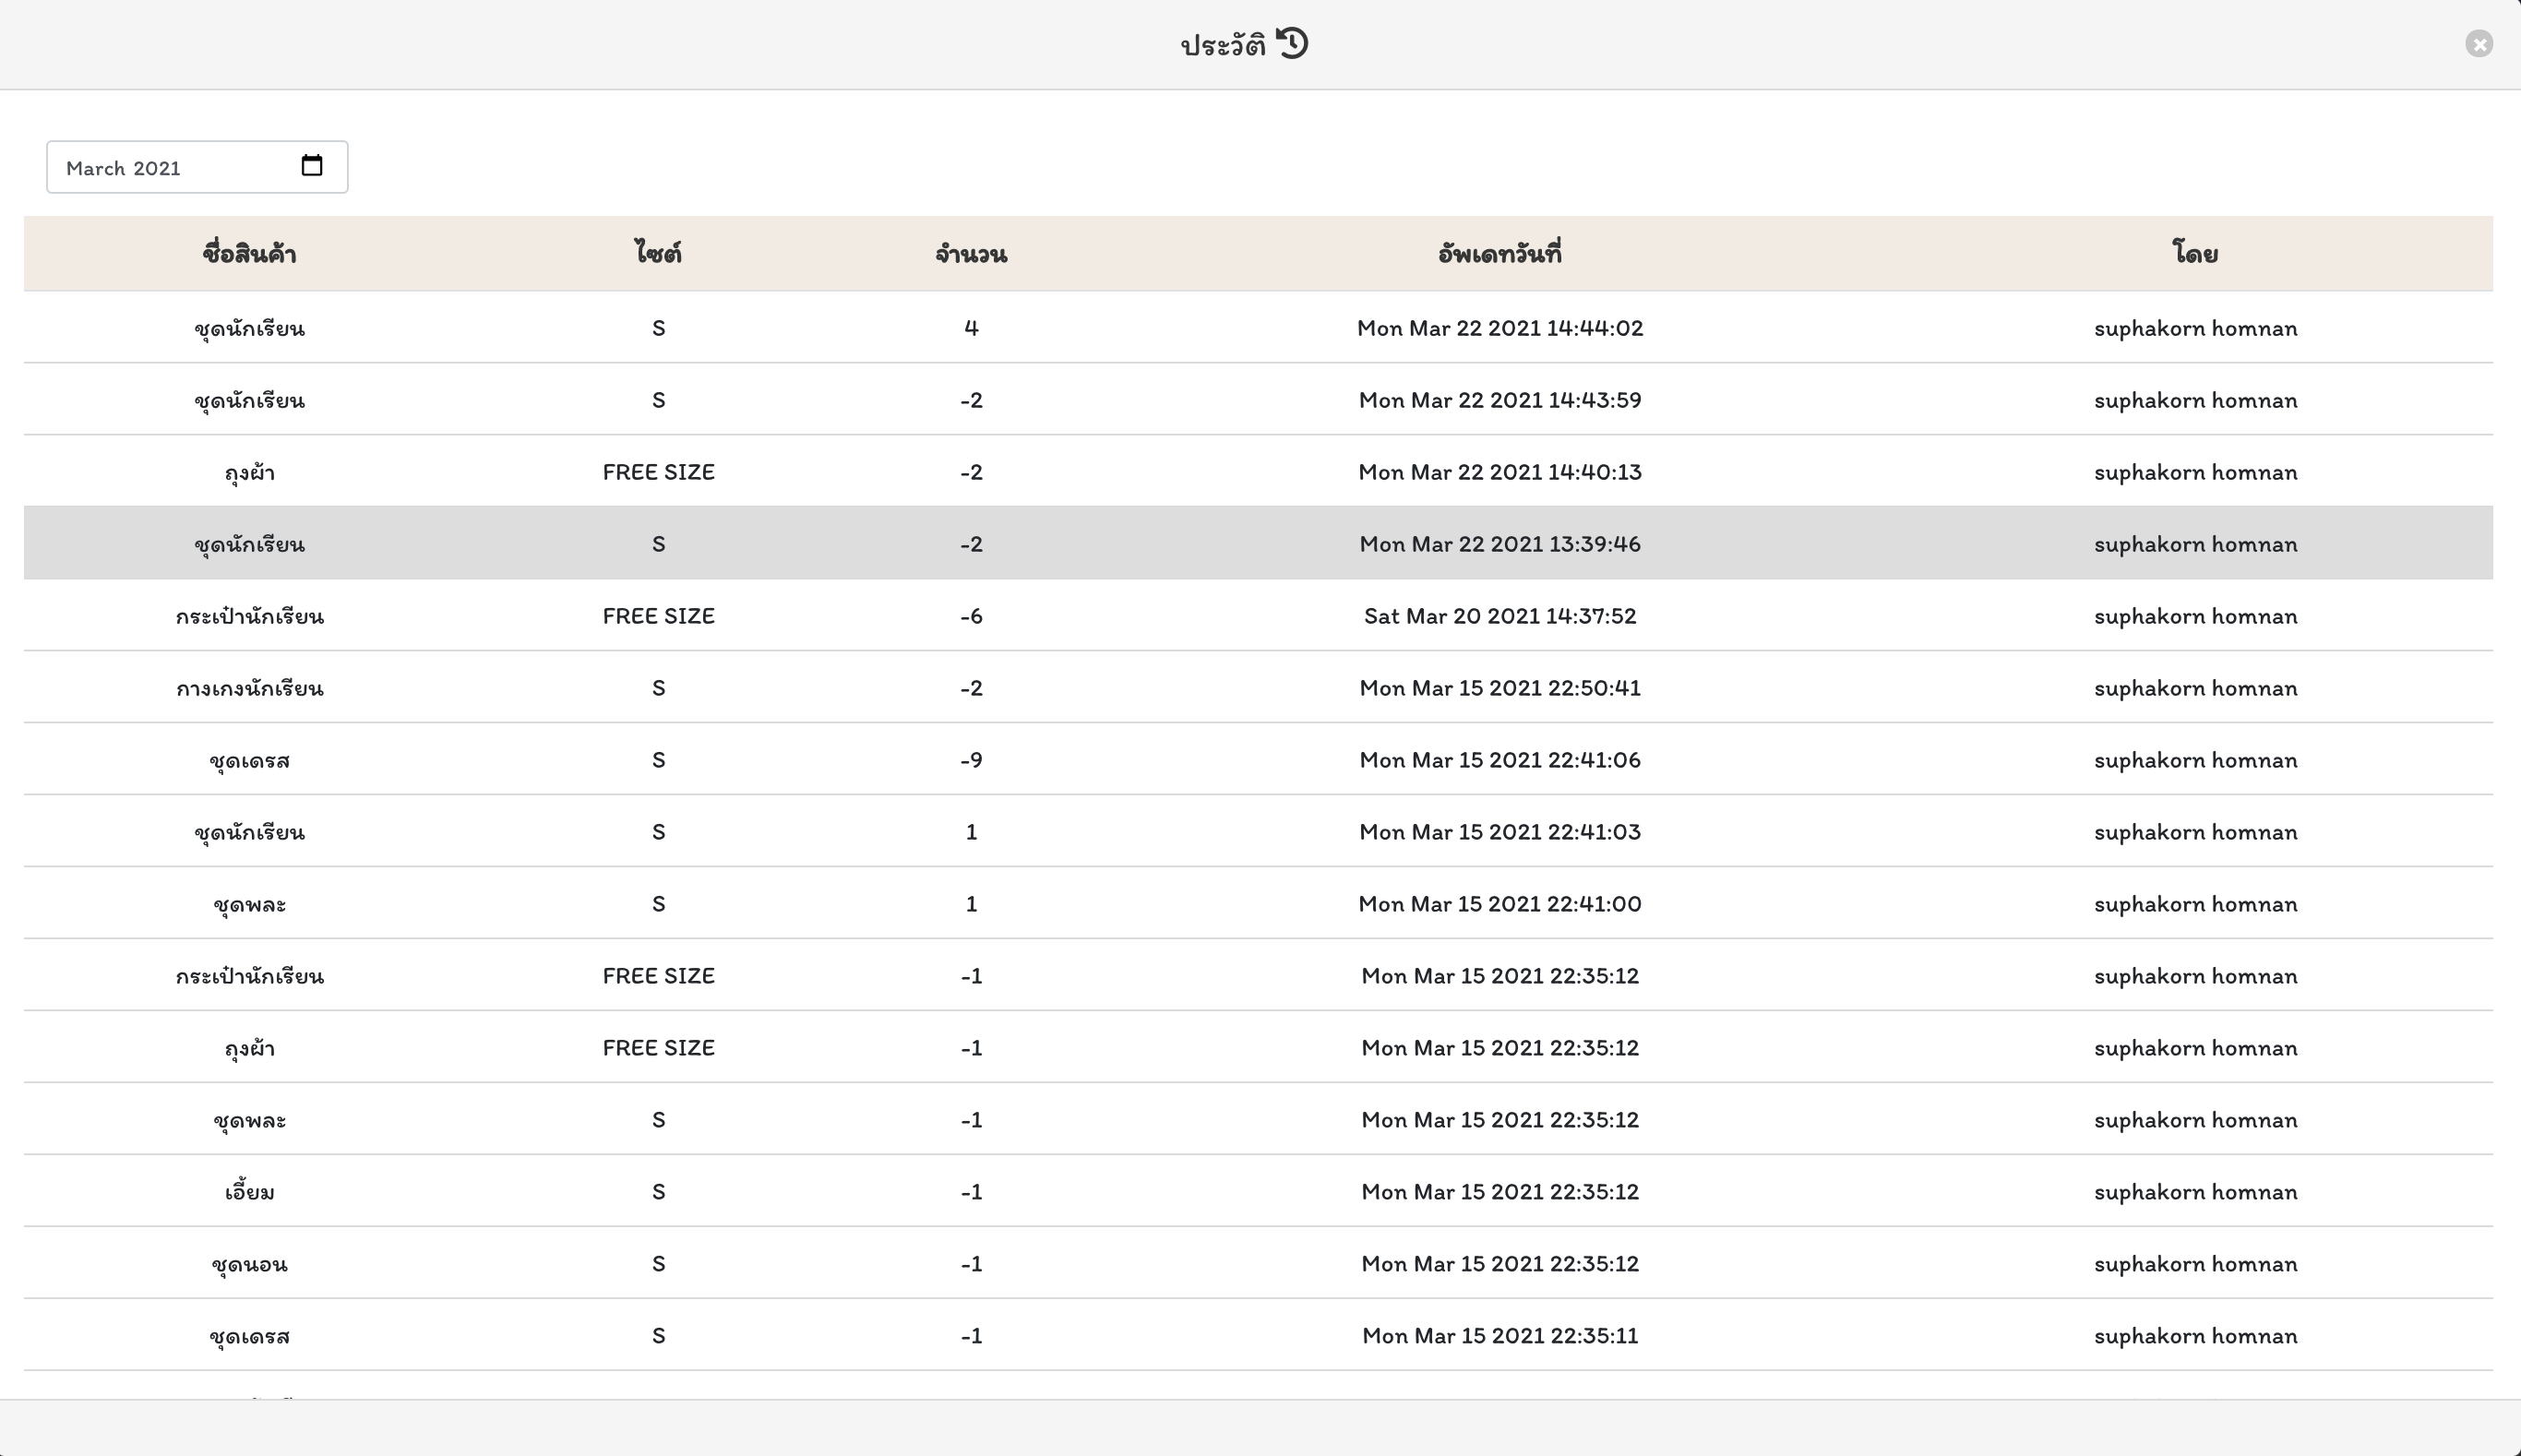
\includegraphics[width=\linewidth]{images/historyStock.png}
      \end{center}
      \caption[หน้าแสดงประวัติการเพิ่มลดของ]{หน้าแสดงประวัติการเพิ่มลดของ}
      \label{fig:HistoryStock}
    \end{figure}
  
  \item  Payment คือ หน้าที่ใช้จัดการกับใบแจ้งยอด(ค้างชำระ)กับใบเสร็จ(ชำระแล้ว) ประวัติการจ่ายเงินค่าภายในnursery หน้าหลักสำหรับระบบบัญชี(รูปที่~\ref{fig:Payment}) หน้านนี้จะแสดงข้อมูลtransactionของทาง nursery (ค่าเริ่มต้นจะเป็นสถานะค้างชำระ) สามารถเปลี่ยนสถานะสำหรับการแสดงผลได้ โดยเลือกที่ input ทางมุมซ้าย 
  การเพิ่มtransaction สามารถทำได้ผ่านหน้าประวัติ(รูป~\ref{fig:Profile}) จากนั้นเลือกเด็กที่ต้องการจะทำรายการ เมื่อเลือกได้แล้วให้กดที่ปุ่มสีเขียว
  หลังจากนั้นระบบจะนำผู้ใช้มายังหน้าเพิ่มรายการบัญชี (รูป~\ref{fig:CreatePayment}) ซึ่งหน้านี้จะให้ผู้ใช้กรอกข้อมูลที่จำเป็นในการทำใบแจ้งยอดรายการ ให้ผู้ใช้กรอกข้อมูลให้ครบถ้วน หลังจากนั้นให้กดบันทึก
  เมื่อกลับมาหน้าบัญชี(รูปที่~\ref{fig:Payment}) รายการที่เพิ่มเข้าไปก็จะแสดงบนหน้าบัญชี หากผู้ใช้ต้องการพิมพ์ใบแจ้งยอดให้ผู้ใช้เลือกรายการที่จะพิมพ์ หลังจากนั้นกดที่ปุ่มสีฟ้าบริเวณด้านขวาสุด
  ระบบจะพาไปยังหน้าพิมพ์ใบแจ้งยอดที่ผู้ใช้เลือกมา(รูป~\ref{fig:invoicePage}) 
  ในส่วนการเปลี่ยนสถานะจากค้างชำระเป็นชำระแล้ว สามารถทำได้โดยการกดปุ่มชำระค่าใช้จ่ายในหน้าบัญชี(รูปที่~\ref{fig:Payment}) หลังจากนั้นระบบจะนำผู้ใช้มายังหน้าอัพเดตรายการ(รูป~\ref{fig:updatePayment})
  หน้านี้จะให้ผู้ใช้กรอกจำนวนเงินที่ทางลูกค้าชำระมาแล้ว(หากเงินที่ชำระมีค่าน้อยกว่า เงินที่ต้องชำระทั้งหมด สถานะจะยังคงค้างชำระเหมือนเดิมแต่จะมีข้อมูลใบเสร็จที่แนบไฟล์มาเพิ่มขึ้นยังระบบที่เก็บข้อมูล)และจะมีให้แนบรูปใบเสร็จ(หากไม่มีรูปเสร็จหรือมีการแถบใบเสร็จภายนอก ให้กดที่ปุ่มแนบสลิปใบเสร็จส่งแยกภายนอก)
  เมื่อกรอกข้อมูลครบให้กดบันทึกก็จะเป็นอันเสร็จสิ้นการอัพเดตรายการ หากผู้ใช้ต้องการจะพิมพ์ใบเสร็จ
  ให้ผู้ใช้เลือกสถานะเป็นชำระแล้ว หลังจากนั้นให้เลือกรายการที่ต้องการพิมพ์ เมื่อเลือกเสร็จให้กดที่ปุ่มสีฟ้า
  หลังจากนั้นระบบจะนำผู้ใช้ไปยังหน้าพิมพ์ใบเสร็จ (รูป~\ref{fig:slipPage}) 

  \begin{figure}
    \begin{center}
    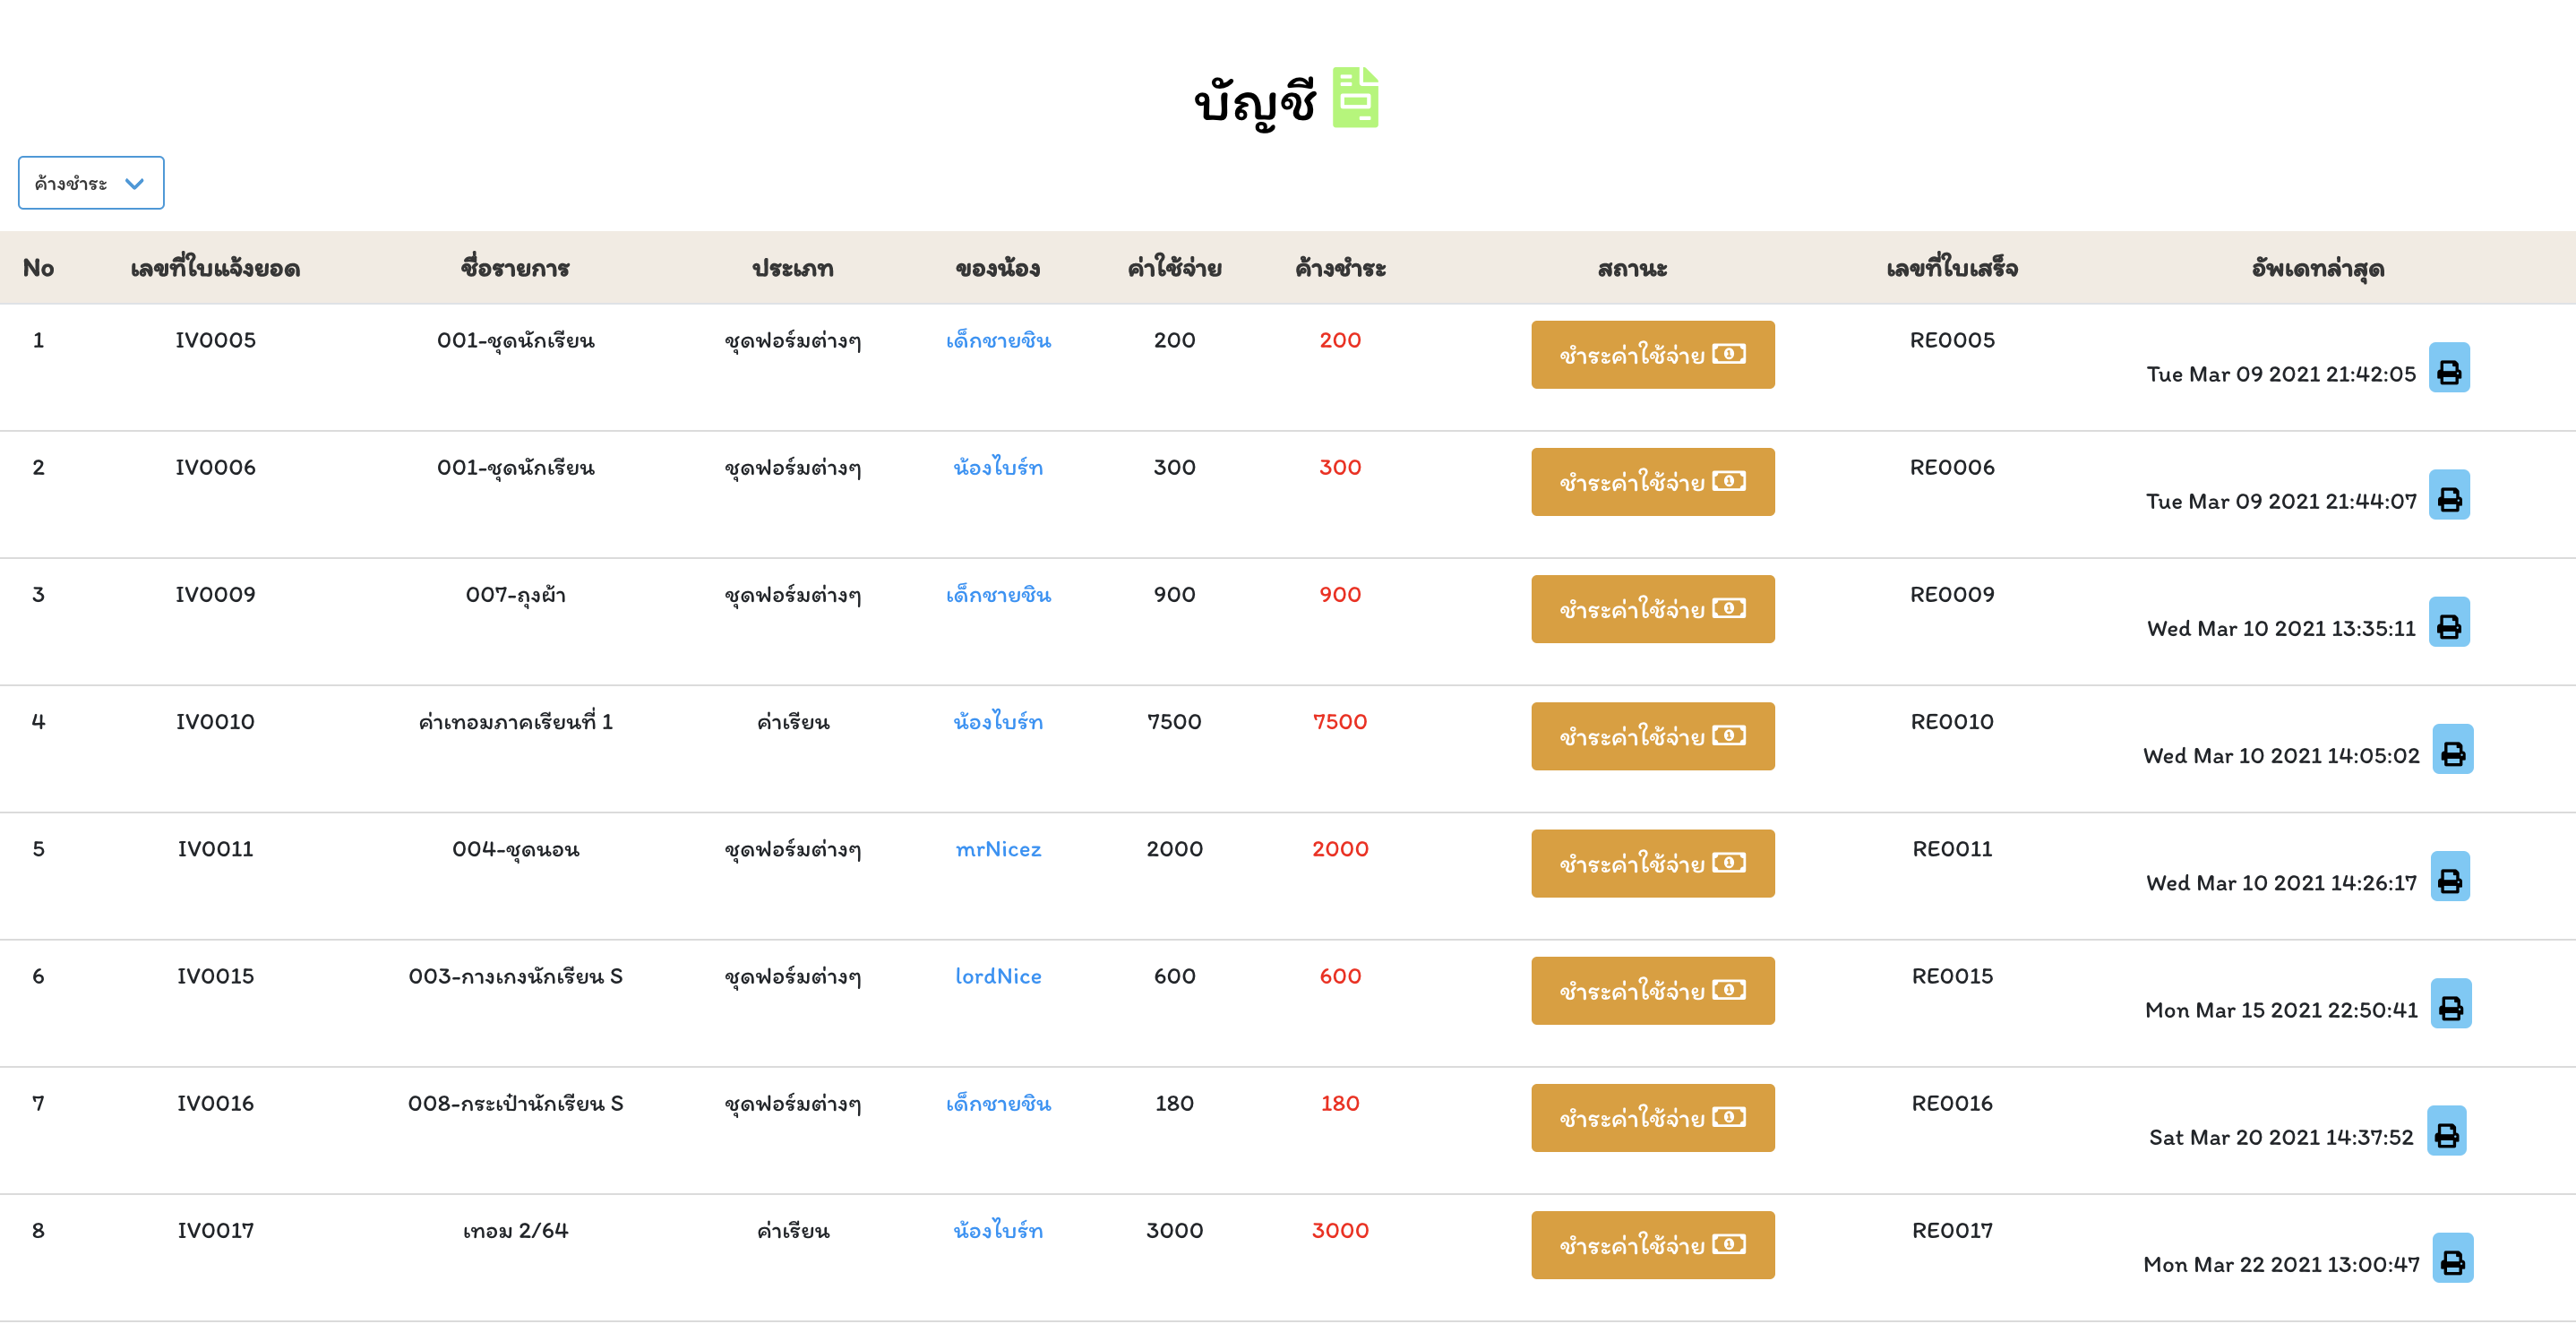
\includegraphics[width=\linewidth]{images/Payment.png}
    \end{center}
    \caption[หน้าแสดงรายการบัญชี]{หน้าแสดงรายการบัญชี}
    \label{fig:Payment}
  
    \end{figure}




  \begin{figure}
    \begin{center}
    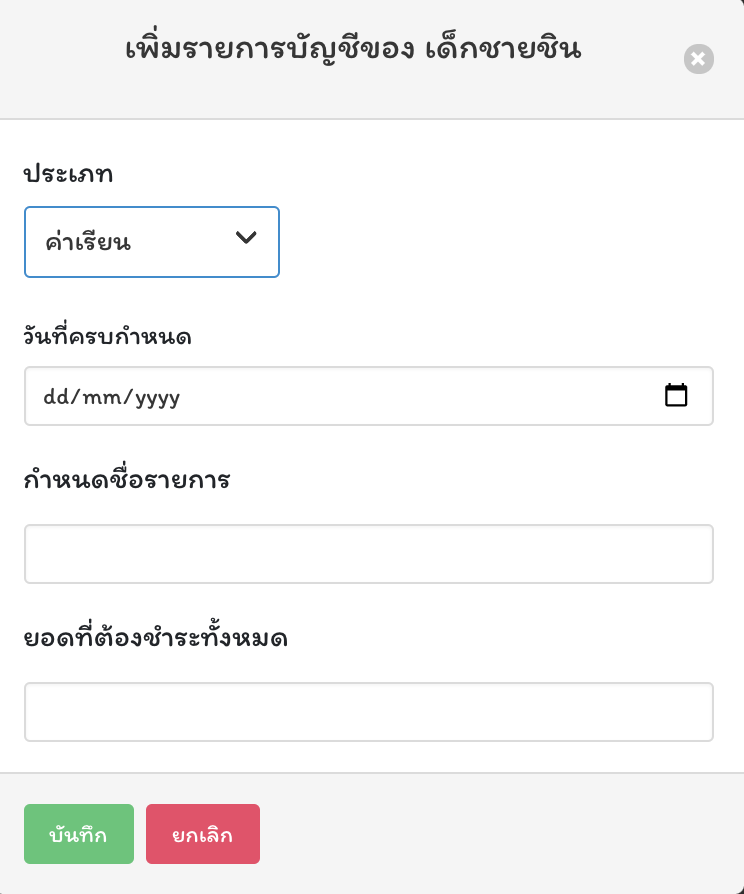
\includegraphics[scale=0.75]{images/CreatePayment.png}
    \end{center}
    \caption[หน้าเพิ่มรายการบัญชี]{หน้าเพิ่มรายการบัญชี}
    \label{fig:CreatePayment}
    \end{figure}


  \begin{figure}
    \begin{center}
    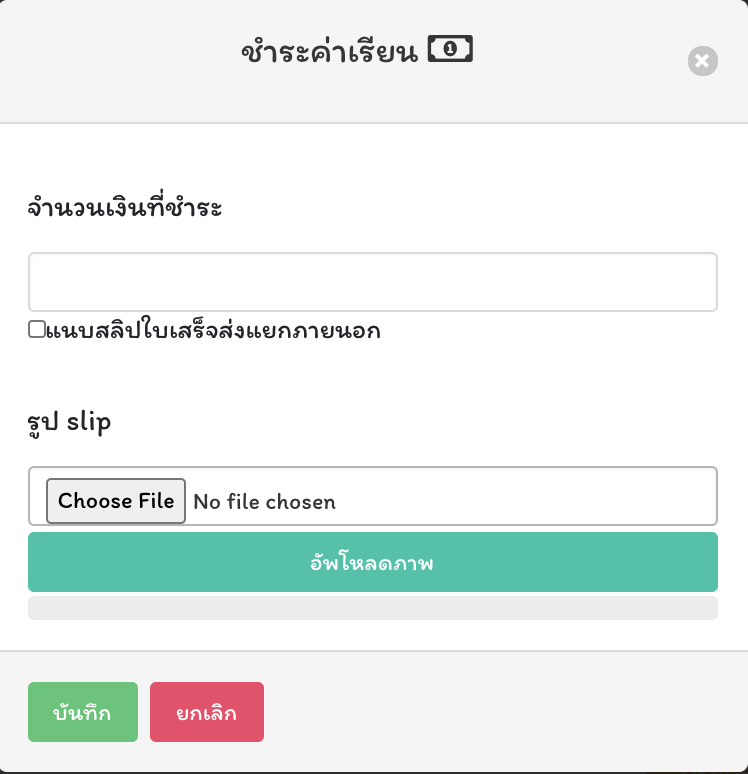
\includegraphics[scale=0.75]{images/UpdatePayment.png}
    \end{center}
    \caption[หน้าชำระค่าใช้จ่าย]{หน้าชำระค่าใช้จ่าย}
    \label{fig:updatePayment}
    \end{figure}

    \begin{figure}
      \begin{center}
      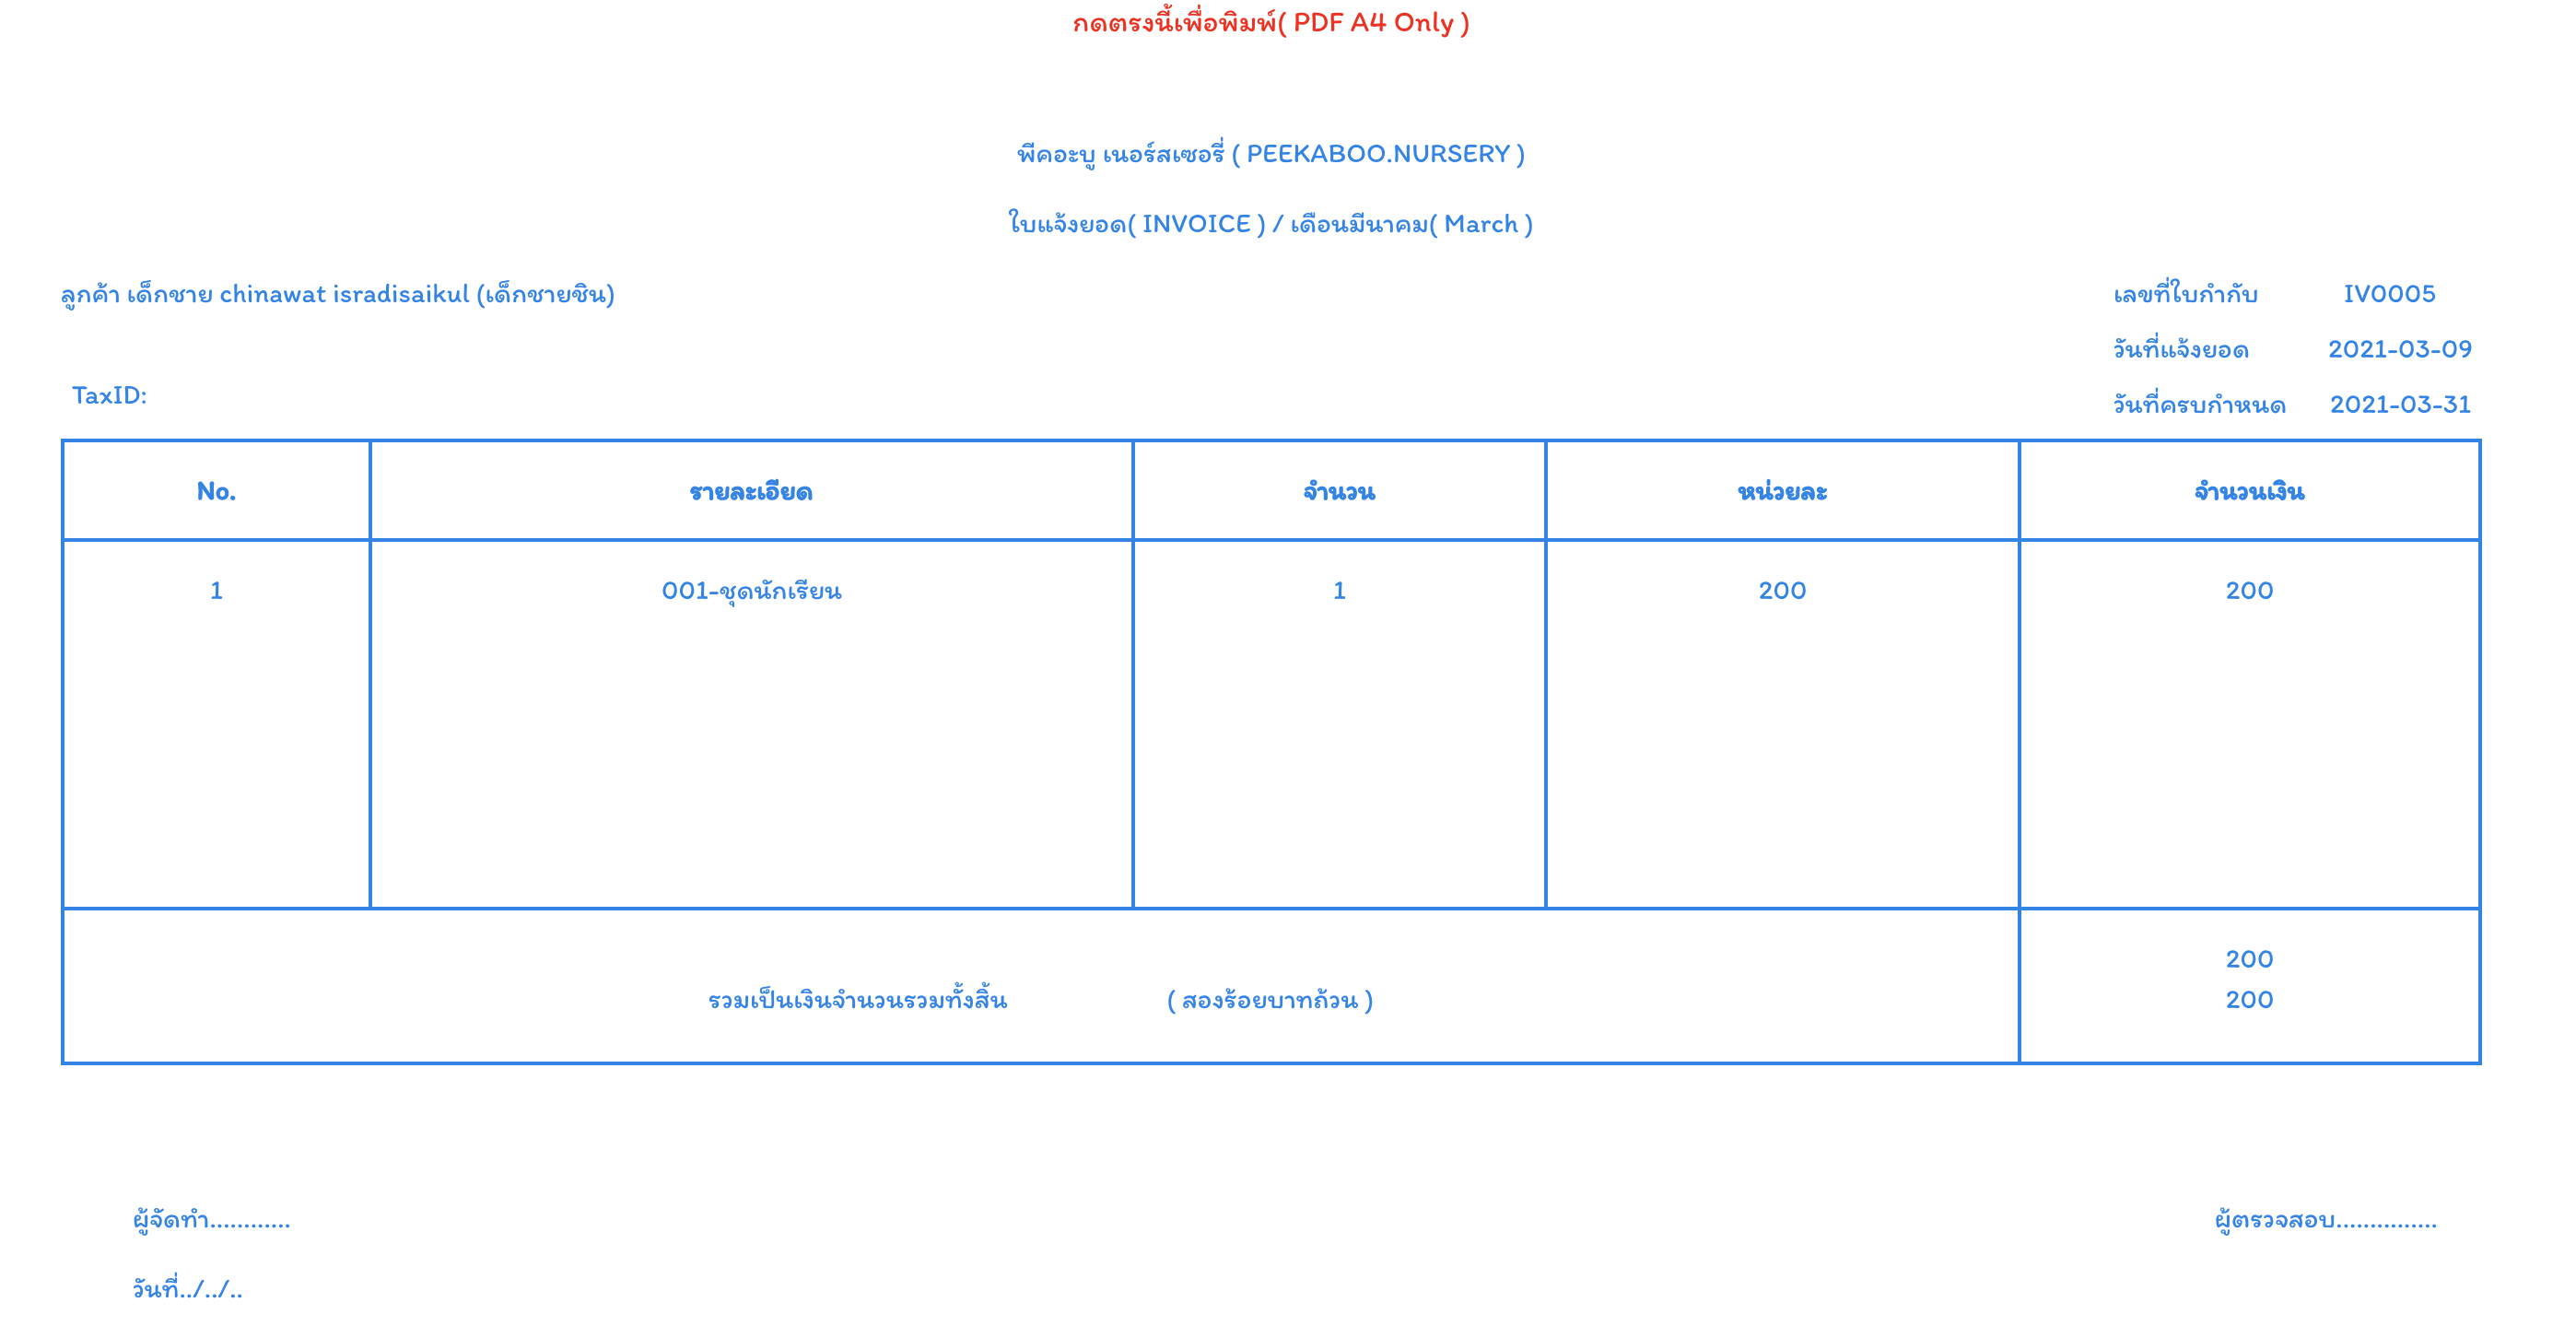
\includegraphics[width=\linewidth]{images/invoicePage.png}
      \end{center}
      \caption[หน้าปริ้นใบแจ้งยอด]{หน้าปริ้นใบแจ้งยอด}
      \label{fig:invoicePage}
      \end{figure}

    \begin{figure}
      \begin{center}
      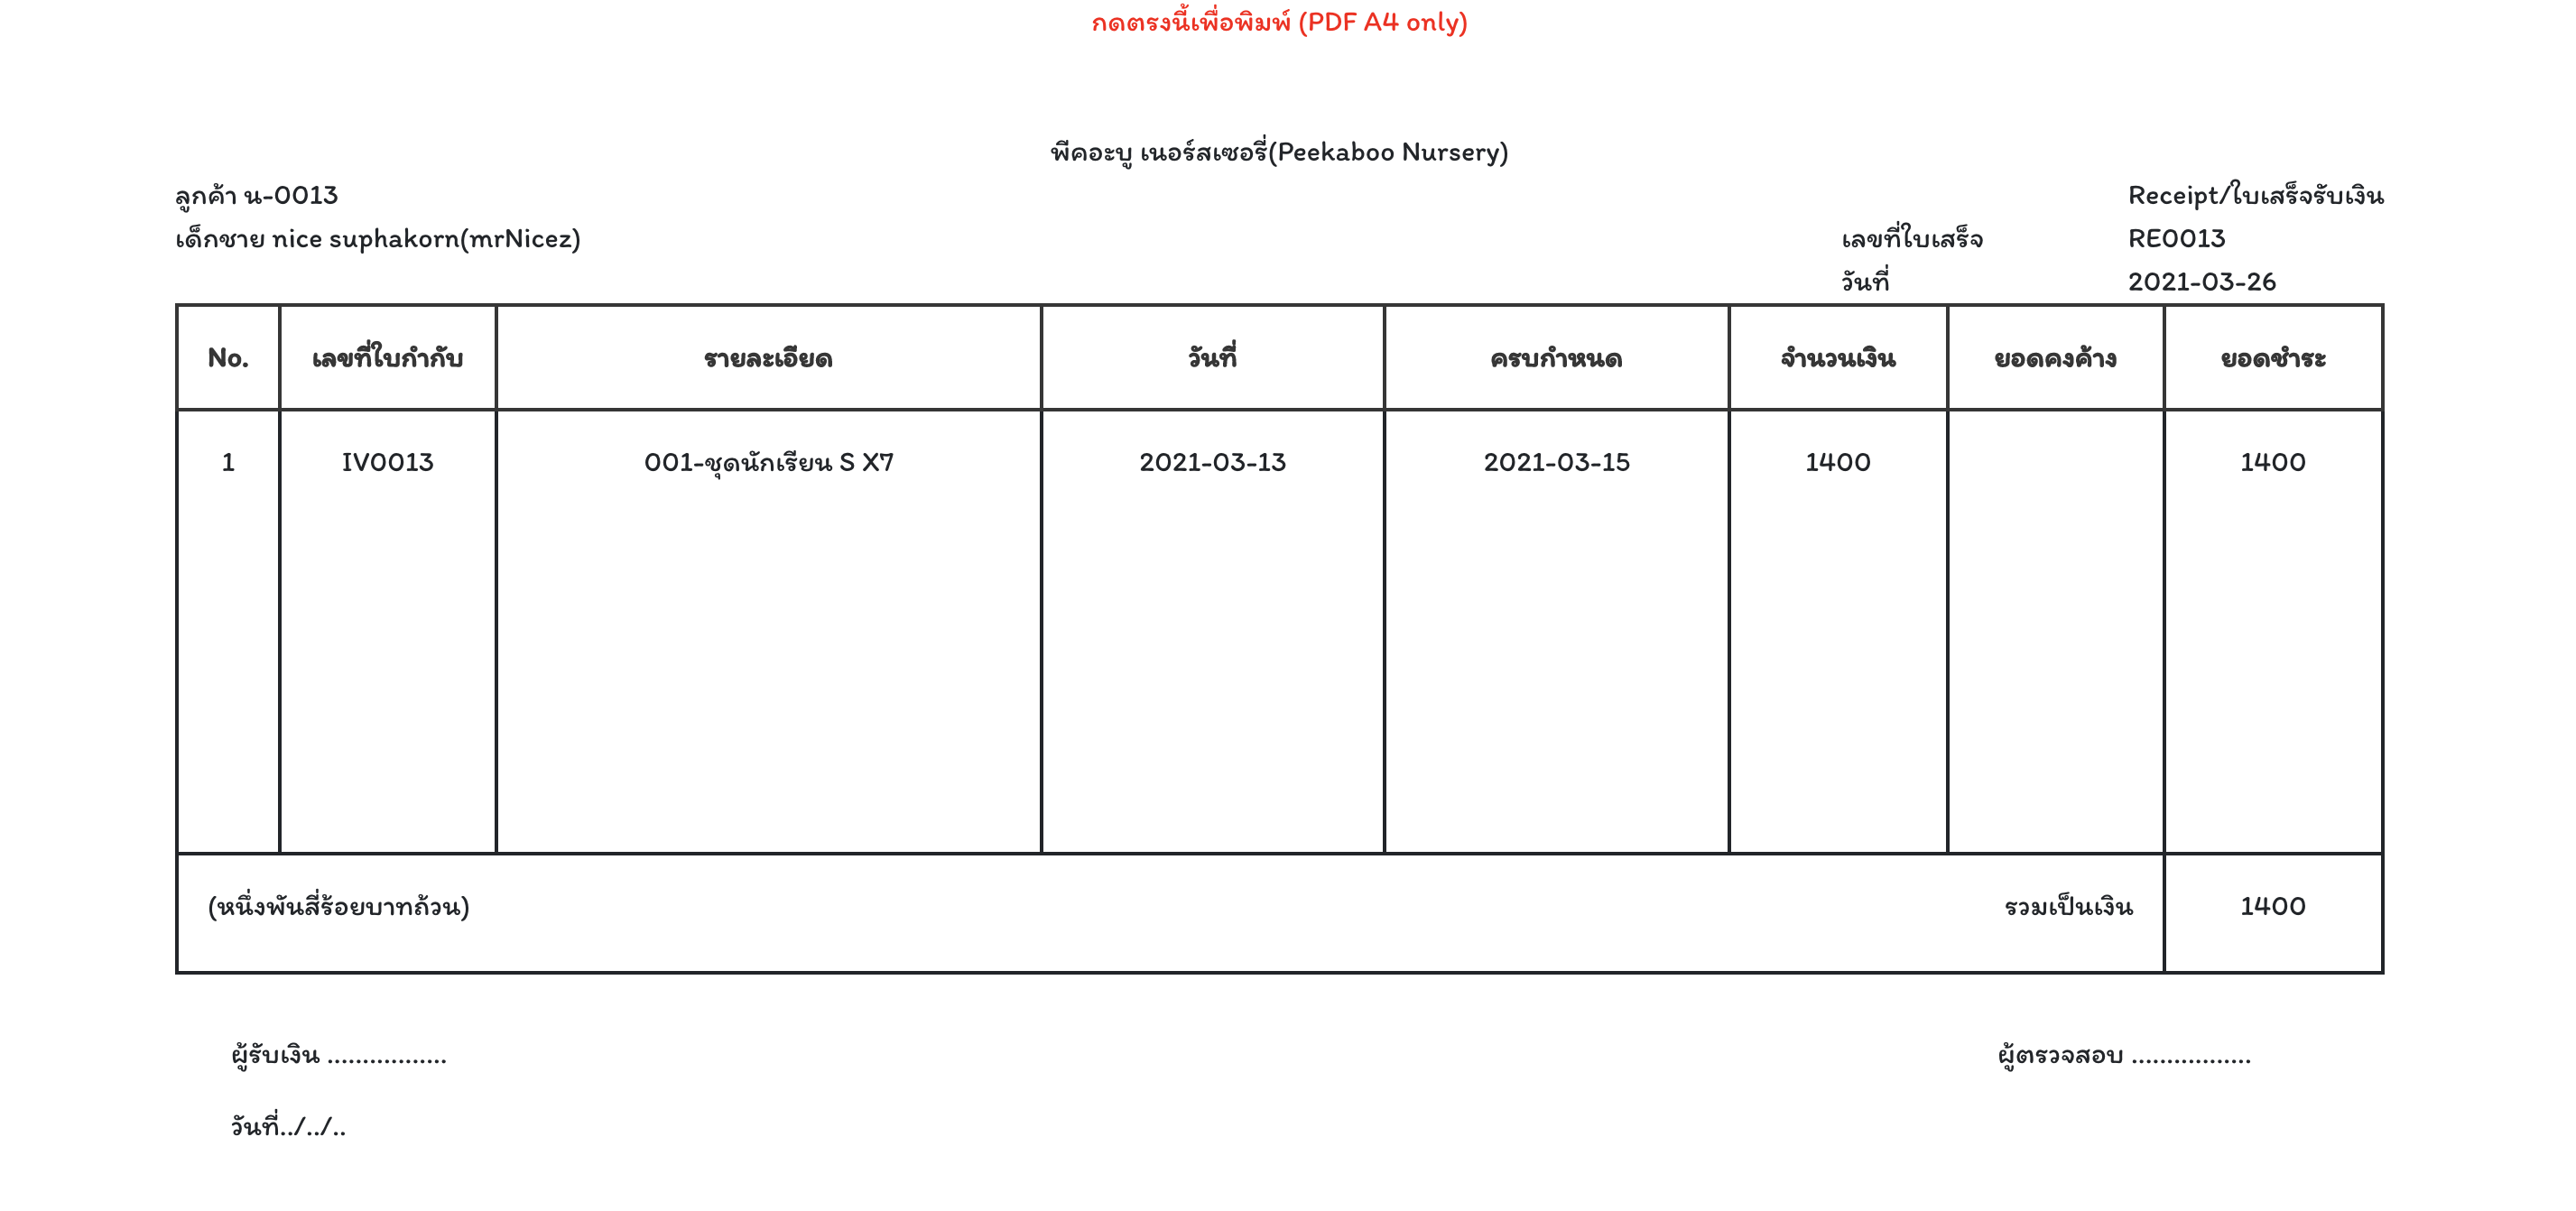
\includegraphics[width=\linewidth]{images/slipPage.png}
      \end{center}
      \caption[หน้าปริ้นใบเสร็จ]{หน้าปริ้นใบเสร็จ}
      \label{fig:slipPage}
      \end{figure}
\end{itemize}
\CIreply{ย้ายรูปมาแทรกในส่วนของ text ให้เหมาะสม}

\subsection{Architecture}

ระบบหลักๆที่ทางผู้พัฒนาใช้เป็นระบบแบบ client-server คือทางฝั่ง client จะใช้ React ในการพัฒนาตัวเว็บไซต์ โดยผู้ใช้จะมีการส่ง request มายังฝั่ง server เพื่อที่จะทำงานที่ผู้ใช้ต้องการ ซึ่งฝั่ง server 
จะพัฒนาผ่าน Express.js ทางฝั่งนี้ก็จะ query ข้อมูลจากทางฐานข้อมูลที่เก็บไว้บน MongoDB Atlas เมื่อได้รับข้อมูลแล้วจะทำการส่ง response กลับไปยัง client เพื่อให้ผู้ใช้สามารถทำงานในส่วนที่ต้องการได้

\subsection{APIs Docs}
ในส่วนของ APIs Document ในส่วนของ url ที่จะนำไปใช้ในการเรียกใช้ service สามารถดูที่หัวมุมด้านซ้ายซึ่งเป็น baseURL สำหรับการใช้งาน

ส่วนหากผู้ใช้ต้องการใช้ service ตัวไหนก็เลือกได้จากตารางข้อมูลในรูปภาพ ยกตัวอย่างเช่น ผู้ใช้ต้องการเรียกใช้ service สำหรับ get ข้อมูลสำหรับหน้าเช็คชื่อที่ใช้แสดงในตารางเช็คชื่อ
ซึ่งการเรียกใช้ก็คือ นำurl "localhost:8000/api/attendance/getChild" ไปเรียกใช้แล้ว ก็ต้องกรอก params ที่ตัวserviceต้องการ paramsที่ตัวserviceนี้ต้องการคือ room(ห้องเรียน), date(วันที่เลือก), amount\_day(จำนวนวันในเดือนที่เลือก)

(รูปที่~\ref{fig:ApiDocs1}, \ref{fig:ApiDocs2})

\section{ขั้นตอนการดำเนินงาน}
\subsection{Discovery}
\begin{itemize}
  \item สำรวจและสอบถามปัญหาจาก stakeholder
  \item นำปัญหาต่างหรือ requirements มาวิเคราะห์
  \item สรุปผลแล้วนำ requirements ที่ได้จากการวิเคราะห์ไปทำต่อในขั้นตอนถัดไป
\end{itemize}

\subsection{Design}
\begin{itemize}
  \item ออกแบบหน้า UI/UX โดย Adobe XD
  \item ออกแบบฐานข้อมูลโดย Draw.io
\end{itemize}

\subsection{Develop}
\begin{itemize}
  \item สร้าง database
  \item เขียน APIs ตามที่ได้ design มาในขั้นตอนก่อนหน้า
  \item เขียน frontend แล้วทดสอบยิง APIs ไปยังฝั่ง Backend
  \item เชื่อมโค้ด frontend กับ backend ผ่าน APIs
\end{itemize}

\subsection{Testing}
\begin{itemize}
  \item ทดสอบระบบในแต่ละฟีเจอร์ว่าสามารถใช้งานได้ตามที่ต้องการหรือไม่
\end{itemize}


  \begin{figure}
    \begin{center}
    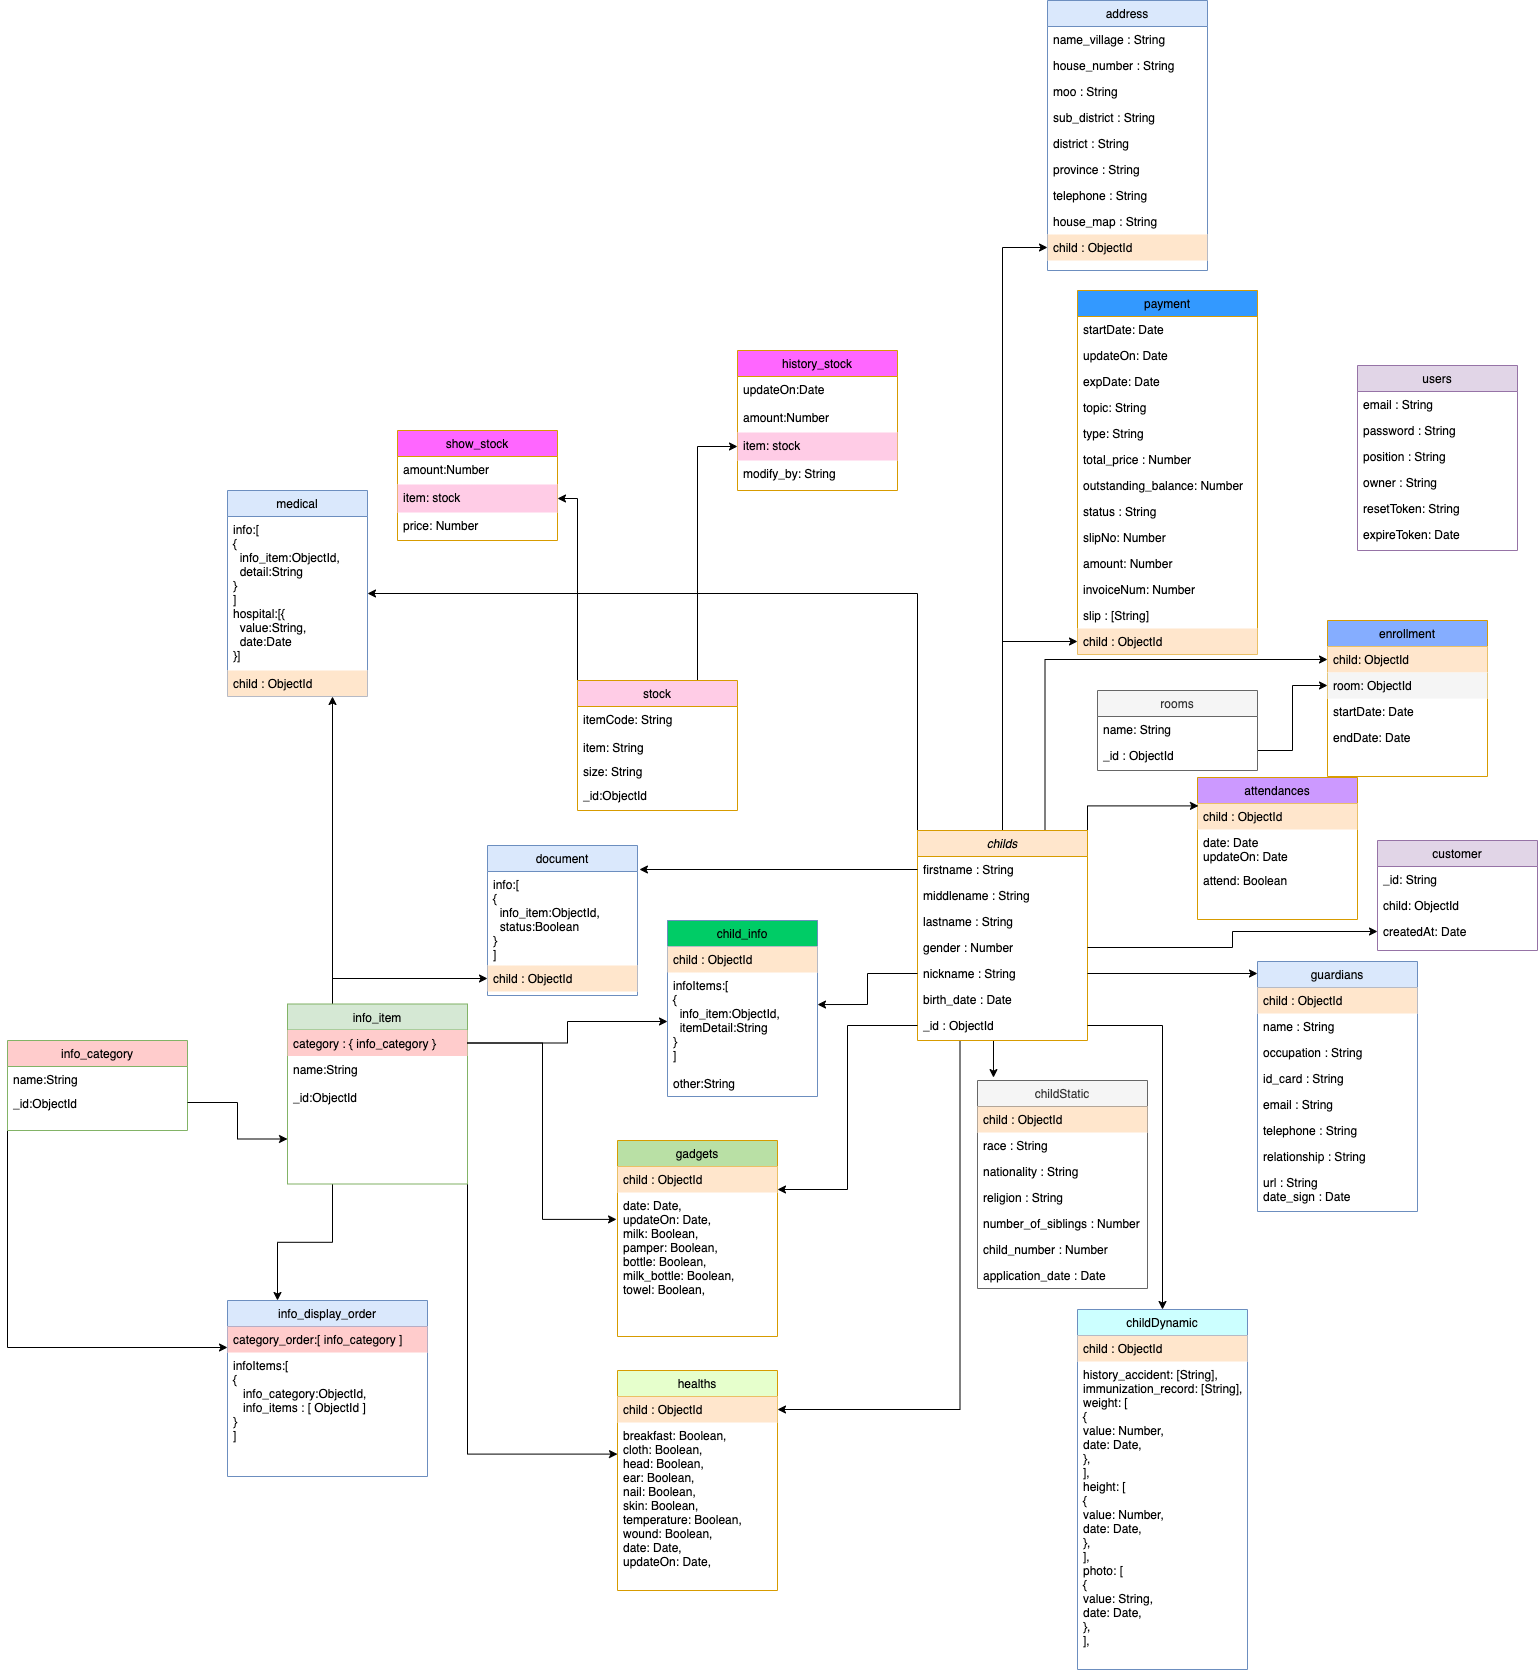
\includegraphics[height=1.0\textheight]{images/NurseryDiagram.png}
    \end{center}
  \caption{แผนภาพแสดงรายละเอียดฐานข้อมูลของระบบ}
  \label{fig:DatabaseDiagram}
\end{figure}
  
  \begin{landscape}
    \begin{figure}
      \begin{center}
        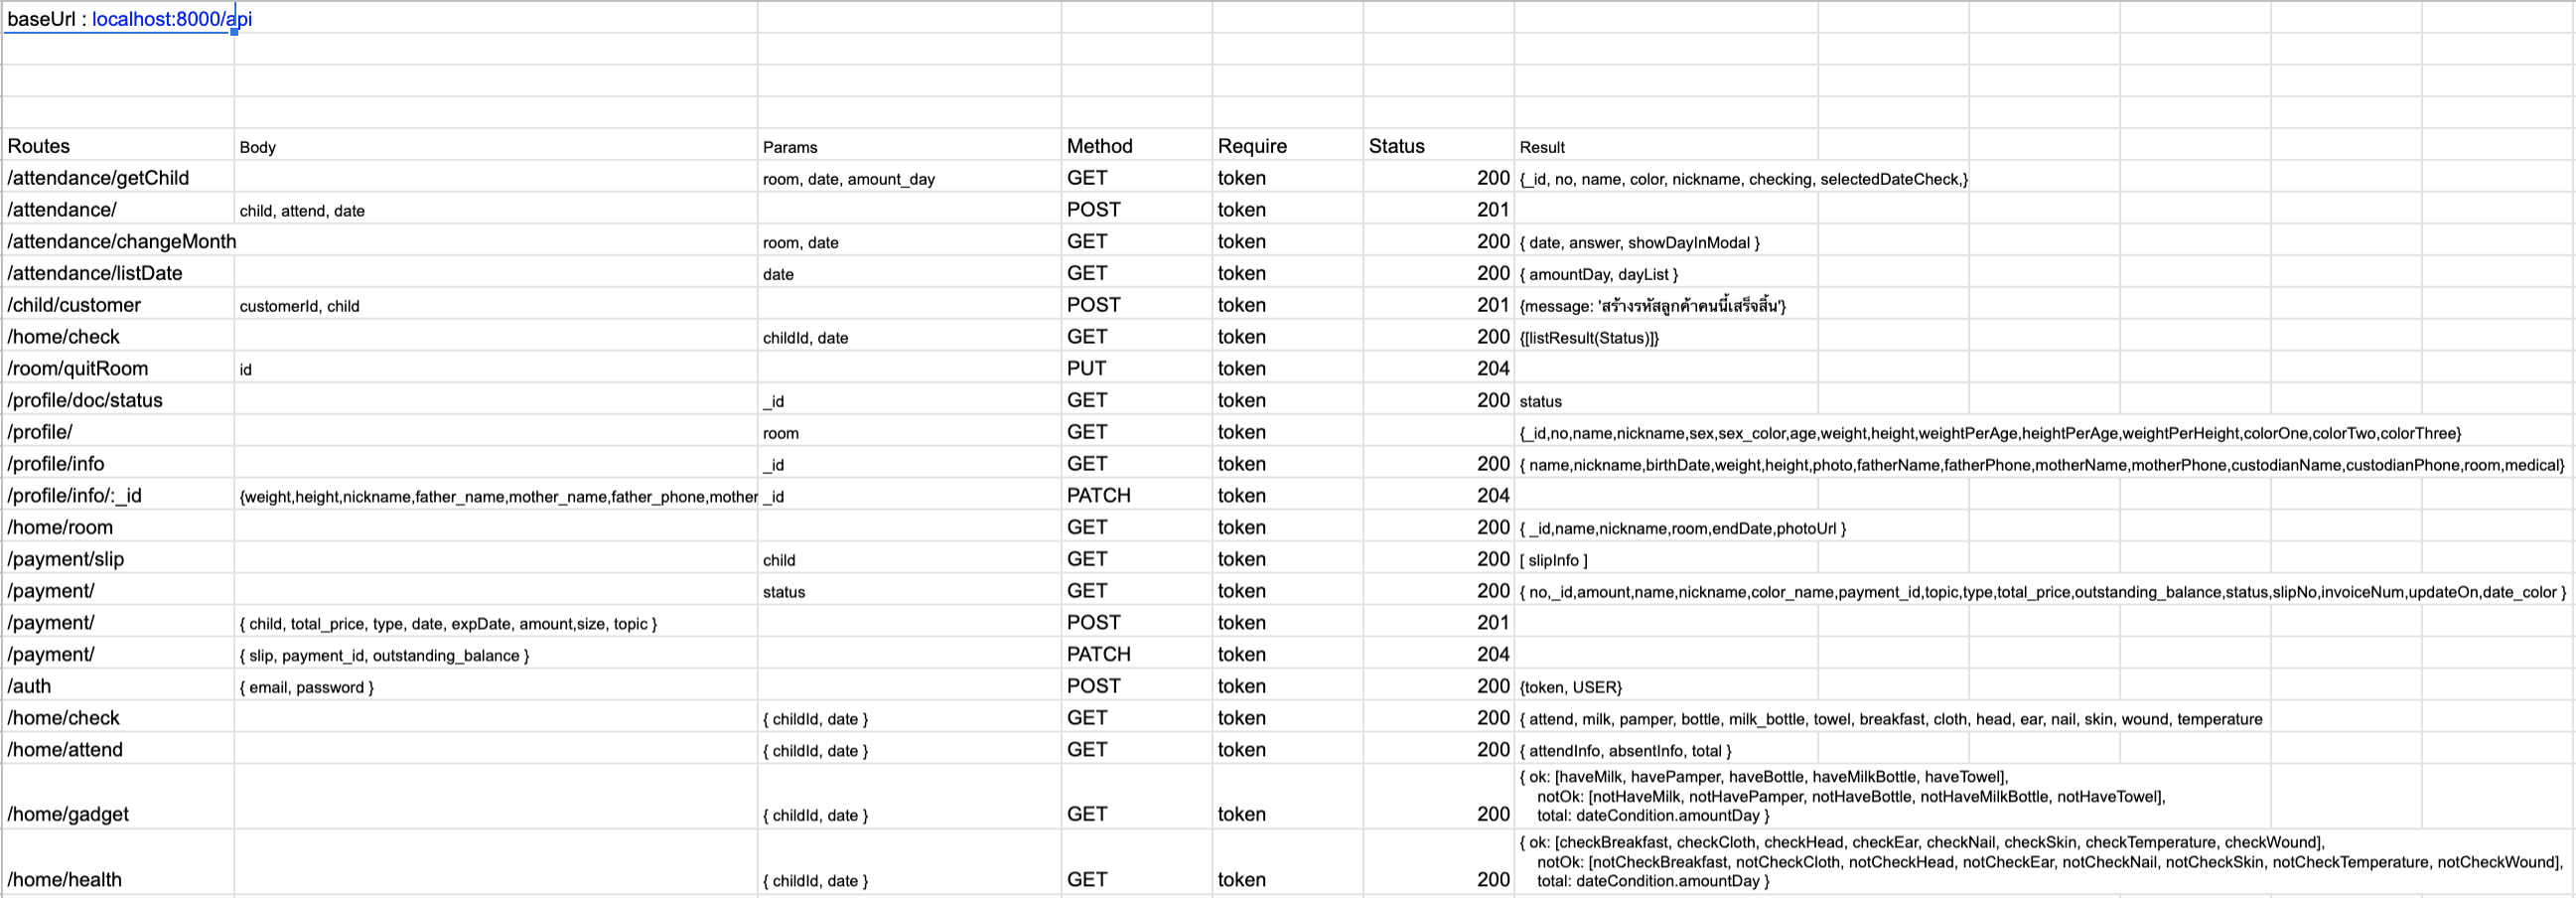
\includegraphics[width=\linewidth]{images/ApiDocOne.png}
      \end{center}
      \caption[ตารางแสดง API Document 1]{ตารางแสดง API Document 1}
      \label{fig:ApiDocs1}
    \end{figure}
  \end{landscape}
  
  \begin{landscape}
    \begin{figure}
      \begin{center}
        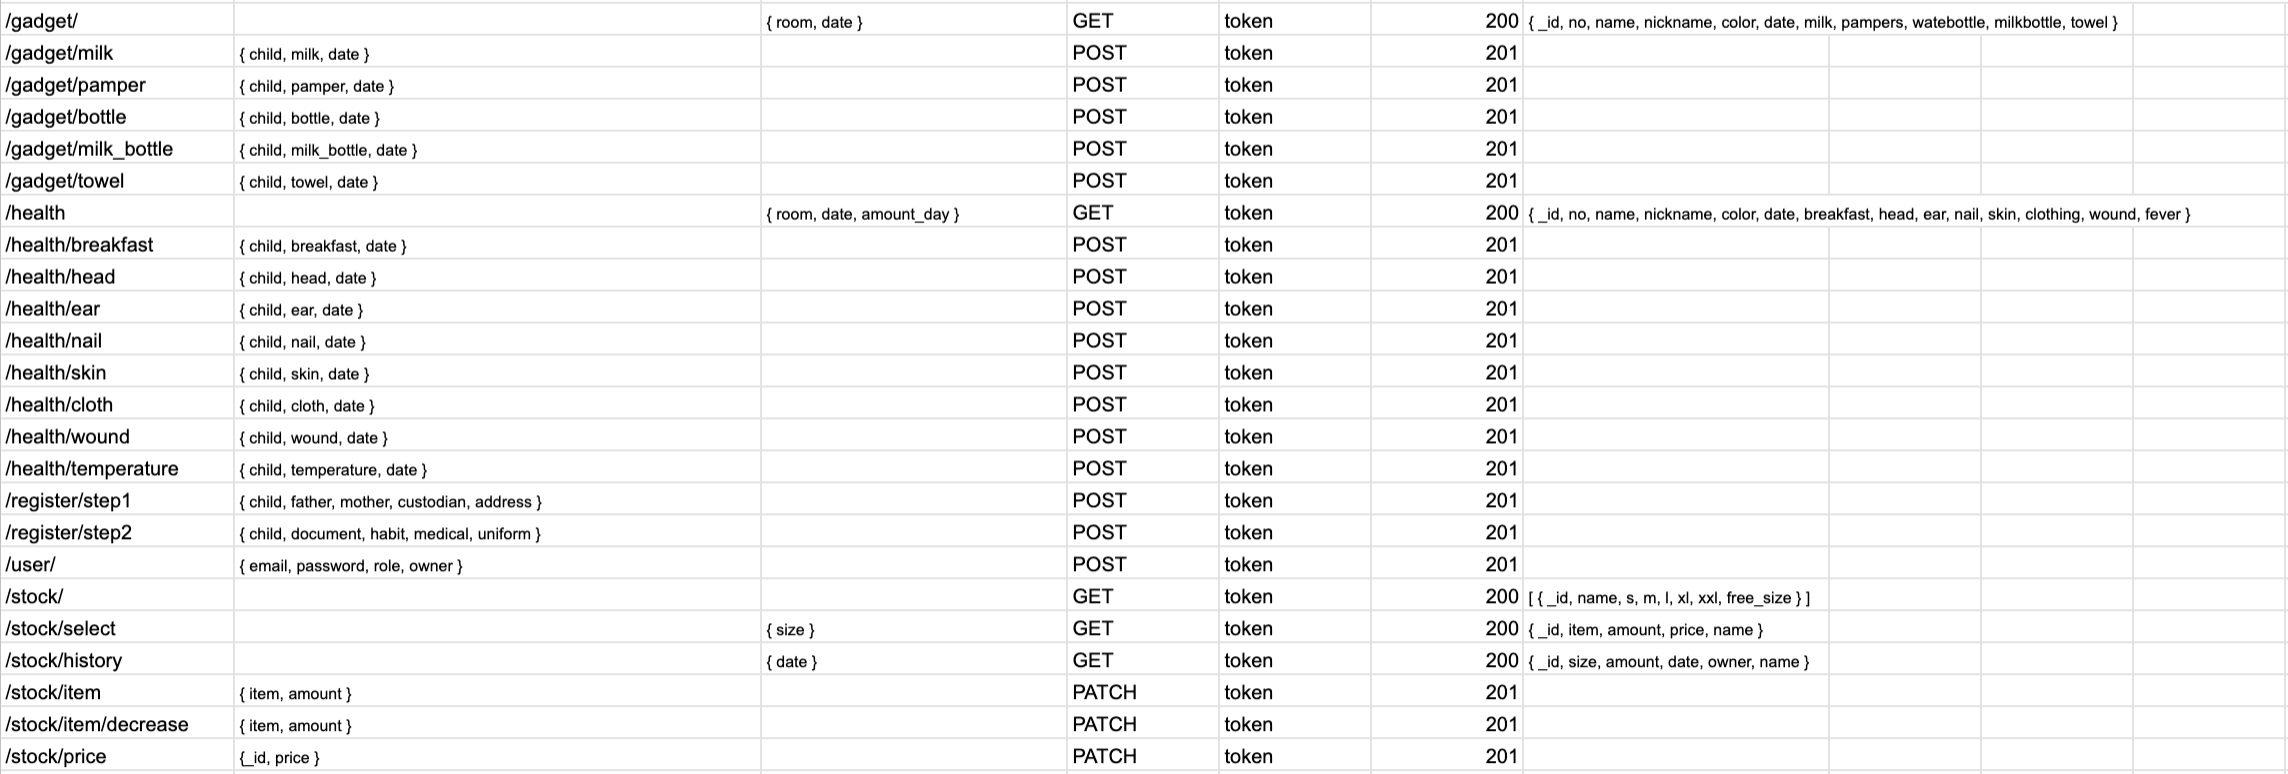
\includegraphics[width=\linewidth]{images/ApiDocTwo.png}
      \end{center}
      \caption[ตารางแสดง API Document 2]{ตารางแสดง API Document 2}
      \label{fig:ApiDocs2}
    \end{figure}
  \end{landscape}